% Default language option is [thaithesis]. The other possible option is [engthesis].
% Default format option is [ugrad]. Other possible options are [master,doctor].
\documentclass[a4paper]{ubu}
%\documentclass[a4paper,engthesis,master]{chula}

% List all required packages here
\usepackage{float}            % for floating figures
\usepackage{amsmath}            % for math related environment
\usepackage{amsfonts}           % fonts for math
\usepackage{listings}           % for psuedocode, lines of codes
\usepackage{caption}
\usepackage[labelformat=simple]{subcaption}
\renewcommand\thesubfigure{(\alph{subfigure})}    % for (a) in subcaption
\usepackage{enumitem}
\usepackage{graphicx}
\usepackage{wrapfig}            % for figures wrap inside text paragraph
\usepackage{pdfpages}           % for including pdf pages
\usepackage{verbatim}           % for block comment
\usepackage{multicol}

\usepackage{standalone}         % for proposal text inclusion
\usepackage{pgfgantt}           % for gantt chart

\usepackage{array}
\usepackage{xcolor,colortbl}

\newcommand*\rot{\rotatebox{90}}

\usepackage{xltxtra}
\usepackage{fontspec}
\defaultfontfeatures{Scale=1.6}
\setmainfont[Script=Thai]{TH Sarabun New}     % Thai alphabet
\XeTeXlinebreaklocale “th_TH”     % Thai alphabet
\XeTeXlinebreakskip = 0pt plus 1pt


% listings format
\lstset{
basicstyle=\ttfamily,
numbers=left,
numberstyle=\small,
breaklines=true,
xleftmargin=.1\linewidth,
frame=single,
columns=fullflexible,
captionpos=b,
showstringspaces=false
}

\usepackage{tikz}
\usetikzlibrary{shapes,positioning,arrows}

%%------------------------------------------------------------
%%-               SETTING THESIS PARAMETERS                  -
%%------------------------------------------------------------
\thesistitle                              % set the thesis tile (use {\wbr} for word break)
{แอปพลิเคชันค้นหายาเพื่อคุณ} % Thai Title
{(Drugiden)}      % English title (auto upper case)

\authortitle                            % set the title of the author, e.g., Mr., Miss, Dr. etc.
{นาย}                                   % Thai Title of the author
{Mr.}                                   % English Title of the author
\thesisauthor                           % set the author name (must not include title (Mr., Miss, Dr., etc.)
{กฤษณะ ชินโคตร}                          % Author name in Thai
{Kritsana Chinnacort}                  % Author name in English

\advisor                                               % set the advisor
{อาจารย์ ดร.เกรียงศักดิ์ ตรีประพิณ}               % Advisor name in Thai
{ดร.เกรียงศักดิ์ ตรีประพิณ}                          % Advisor name in Thai with abbrev. title
{Kriengsak Treeprapin, Ph.D.}  % Advisor name in English
{KRIENGSAK TREEPRAPIN, Ph.D.}          % Advisor name in English with abbrev. title 
                                                       % (Capital letters except Ph.D.))

%% If the thesis has co-advisor, use this optional command
%% Uncomment if necessary
%\coadvisor
%{อาจารย์ ดร.ภควรรณ ปักษี}  % Co-Advisor name in Thai
%{อ. ดร.ภควรรณ ปักษี}  % Co-Advisor name in Thai with abbrev. title
%{Pakawan Pucksee, Ph.D.}  % Co-Advisor name in English
%{PAKAWAN PUCKSEE, Ph.D.}          % Co-Advisor name in English with abbrev. title 
                                                       % (Capital letters except Ph.D.))

\faculty                                % set the faculty
{วิทยาศาสตร์}                          % name of the faculty in Thai
{Science}                           % name of the faculty in English
\department                             % set the department
{คณิตศาสตร์ สถิติ และคอมพิวเตอร์}                      % name of the department in Thai
{Mathematics Statistics and Computer}                  % name of the department in English
\fieldofstudy                           % set the field of study (สาขาวิชา)
{วิทยาการคอมพิวเตอร์}                      % Field in Thai
{Computer Science}                  % Field in English
\degree                                 % set the degree name
{วิทยาศาสตรบัณฑิต}                   % Degree name in Thai
{Bachelor of Science}                  % Degree name in English
\academicyear{2560}                     % Academic Year (in Thai Calendar)
\authorid{5711404802}                   % ID of the author
\subjID{2301499}							% Course ID for undergrad report
\subjName								% course name
{โครงงานวิทยาศาสตร์}
{Senior project}

\deanname                               % name of the dean
{ดร. ชัชวิน นามมั่น}                       % in Thai
{Chatchawin Namman, Ph.D.}     % in English

% Committee Block
% Speficy the chair/committee/external committee in your selected language
\committee                              % list of committee
{
\CommitteeBlockAdvisor                  % pre-defined value for advisor
\CommitteeBlockCoAdvisor                % pre-defined value for co-advisor
\CommitteeBlock{กรรมการ}{ดร. สุภาวดี หิรัญพงศ์สิน} % examiner
\CommitteeBlock{กรรมการ}{ดร. ไพชยนต์ คงไชย } % examiner
}

%%-------------------------------------------------------------------------------
%%-                               DOCUMENT                                      -
%%-------------------------------------------------------------------------------
\begin{document}

% Thesis starts with Thai Cover
\makethaicover
\newpage

% Followed by English Cover
%\makeenglishcover
%\newpage

% Generate committee page
\makecommittee
\newpage

% Acknowledgement Section
\begin{acknowledgements}
    การพัฒนาโครงงานค้นหายาเพื่อคุณ สำเร็จลุล่วงได้ด้วยความช่วยเหลือจาก ดร.เกรียงศักดิ์ ตรีประพิณ 
    อาจารย์ที่ปรึกษาโครงงานที่ได้ให้คำแนะนำ ทฤษฏี และแนวคิดตลอดจนช่วยแก้ไขข้อบกพร่องต่างๆ 
    โดยตลอด โครงงานนี้สำเร็จสมบูรณ์ ผู้จัดทำโครงการจึงใคร่ขอกราบขอบพระคุณเป็นอย่างสูงไว้ ณ โอกาศนี้
    
    ขอขอบพระคุณอาจารย์ประจำภาควิชาคณิตศาสตร์ สถิติ และคอมพิวเตอร์ คณะวิทยาศาสตร์ทุกท่าน 
    ที่คอยให้คำแนะนำและช่วยเหลือในการศึกษาตลอดปีการศึกษา
    
    ขอขอบพระคุณหน่วยข้อมูลยาและสุขภาพ คณะเภสัชศาสตร์ มหาวิทยาลัยอุบลราชธานี 
    ที่ให้ใช้ฐานข้อมูลการพิสูจน์เอกลักษณ์ยาเม็ดหรือแคปซูลในประเทศไทย

    ขอขอบพระคุณบิดาและมารดาที่ค่อยให้กำลังใจและการสนับสนุนในการพัฒนาโครงงาน 
    คอยสอบถามและคอยห่วงใยเสมอมา
    
    ขอขอบคุณเพื่อนสาขาวิทยาการคอมพิวเตอร์ ชั้นปี 4 รุ่นที่ 18 มหาวิทยาลัยอุบลราชธานีที่ช่วยให้คำแนะนำ 
    คำปรึกษาและเป็นกำลังใจในการทำโครงงานจนสำเร็จลุลวงไปได้ด้วยดี

\end{acknowledgements}

\begin{flushright}
    นายกฤษณะ ชินโคตร
    \vspace{-5mm}
    
    วันที่ 18 เมษายน 61
\end{flushright}

\newpage

% Thai Abstract Section
\begin{thaiabstract}
    โครงงานแอปพลิเคชันค้นหายาเพื่อคุณเป็นการพัฒนาแอปพลิเคชันบนโทรศัพท์สมาร์ทโฟน (Smartphone) 
    ระบบปฏิบัติการแอนดรอยด์ (Android) 
    เพื่อช่วยในการพิสูจน์เอกลักษณ์ยาเม็ดหรือแคปซูลสำหรับเภสัชกรและประชาชนทั่วไป 
    ด้วยการระบุลักษณะทางกายภาพของยา ได้แก่ สี ขนาดด้านยาว รูปทรงและตัวอักษรหรือตัวอักขระบนเม็ดยา 
    หรือข้อมูลทางด้านการผลิต เช่น ชื่อทางการค้า ชื่อสามัญ บริษัทที่จำหน่าย สถานะของยา เป็นต้น 
    โครงงานใช้ Node.js พัฒนาเว็บเซอร์วิส (Web Service) 
    ส่วนเว็บเซอร์วิสทำหน้าที่ติดต่อระหว่างแอพพลิเคชั่นกับฐานข้อมูลการพิสูจน์เอกลักษณ์ยาเม็ดของหน่วยข้อมูลยาและสุขภาพ 
    คณะเภสัชศาสตร์ มหาวิทยาลัยอุบลราชธานี 
    และใช้ Ionic Framework ในการพัฒนาแอปพลิเคชันโดยแอปพลิเคชันที่พัฒนาสามารถระบุลักษณ์รูปทรงยาเม็ดหรือแคปซูลด้วยการค้นหาแบบทั่วไปและแบบขั้นสูง
    และการประมวลผลภาพ (OpenCV) ที่มีแบบจำลอง Support Vector Machines (SVM) 
    ที่ให้ค่าความถูกต้องของแบบจำลองแบบร้อยละ 94.17 และการระบุลักษณะสีด้วยการดูค่า RGB จากจุดพิกเซล (Pixel) 
    และการวัดขนาดด้านยาวจะใช้วัตถุที่รู้ขนาดด้านกว้างและด้านยาวมาช่วยอ้างอิงขนาดด้านยาวของยาเม็ดได้
\noindent
\\คำสำคัญ: การพิสูจน์เอกลักษณ์ยาเม็ด เทคนิคการประมวลผลภาพ แอปพลิเคชันบนโทรศัพท์สมาร์ทโฟน
\end{thaiabstract}
\newpage

% English Abstract Section
%\begin{englishabstract}
This is an introduction to {\LaTeX} starting from the installation, basic typesetting, inserting equations and mathematical symbols.
Later chapters also include the manipulation of figures and tables. The report also includes a basic tutorial for BibTeX.
The format of this report conforms with the thesis format of Chulalongkorn University.

\noindent
Keywords: typesetting, equation 
\end{englishabstract}


%\newpage


% Table of Content
\tableofcontents        % generate table of content
\newpage
\listoftables           % generate list of tables
\newpage
\listoffigures          % generate list of figures
\newpage

% Main Content
\chapter{บทนำ}

\section{ที่มาและเหตุผล }
ปัญหาจากการได้รับประทานยาปลอมหรือยาที่ถูกเพิกถอนทะเบียนเป็นปัญหาใหญ่ในปัจจุบัน เพื่อป้องกันปัญหานี้ก่อนจะมีการใช้ยาใด ๆ ที่ไม่รู้จัก จึงต้องมีการตรวจสอบยาให้ละเอียดก่อน แต่ในปัจจุบันการพิสูจน์เอกลักษณ์ยาเม็ดหรือแคปซูลเป็นไปได้ยาก เนื่องมาจากความคล้ายคลึงกันของยาเม็ดหรือแคปซูลในหลายชนิด ทั้งขนาด สี รูปทรง ชื่อยา เป็นต้น ดังนั้นการพิสูจน์เอกลักษณ์ยาเม็ดหรือแคปซูลจำเป็นต้องอาศัยเภสัชกรหรือผู้เชี่ยวชาญที่มีประสบการณ์และความสามารถในการจดจำในการพิสูจน์เอกลักษณ์ยาเม็ด แต่การจดจำลักษณะของเม็ดยาจำนวนมากและข้อมูลรายละเอียดของยาแต่ละชนิดจำเป็นต้องใช้การอ้างอิงข้อมูลในการพิสูจน์เอกลักษณ์ยาเม็ดที่เชื่อถือได้ เช่น ค้นหาในเว็บไซต์พิสูจน์ยาโดยเฉพาะที่ได้รับการรับรองจากหน่วยงานราชการเป็นต้น 

หน่วยข้อมูลยาและสุขภาพ คณะเภสัชศาสตร์ มหาวิทยาลัยอุบลราชธานี ได้ริเริ่มทำงานวิจัยที่รวบรวมข้อมูลได้แก่ ชื่อการค้า ชื่อสามัญทางยา รูปแบบผลิตภัณฑ์ รูปร่างลักษณะ สัญลักษณ์หรือตัวอักษรบนยาเม็ดหรือแคปซูล สี ขนาดของยาเม็ดและแคปซูล บริษัทผู้ผลิต และบริษัทผู้จำหน่ายโดยเริ่มจากการจัดทำฐานข้อมูลการพิสูจน์เอกลักษณ์ของยาเม็ดและแคปซูลก่อนและได้สร้างเว็บไซต์ Drug Identification Database [13] เพื่อใช้ในการเป็นฐานข้อมูลในการพิสูจน์เอกลักษณ์ยา 

เนื่องจากการใช้เว็บไซต์ Drug Identification Database ยังไม่สามารถรองรับการใช้งานผ่านโทรศัพท์สมาร์ทโฟนและเพื่อความสะดวกของการใช้งาน ผู้พัฒนาจึงได้ทำโครงการแอปพลิเคชันค้นหายาเพื่อคุณที่ผู้ใช้งานสามารถสืบค้นหารายละเอียดยาได้และสามารถถ่ายรูปยาเม็ดเพื่อการพิสูจน์เอกลักษณ์ของยาเม็ดหรือแคปซูลได้โดยไม่ต้องอาศัยเภสัชกรหรือผู้เชียวชาญในการจดจำในการพิสูจน์เอกลักษณ์ยาและสามารถตอบโต้กับผู้ใช้งานได้ทันที โดยใช้ความเป็นโทรศัพท์สมาร์ทโฟนที่สามารถใช้งานได้ที่ทุกที่ทุกเวลา

\section{วัตถุประสงค์}
    
    \begin{enumerate}
        \item เพื่อพัฒนาแอปพลิเคชันที่สามารถการสืบค้นข้อมูลและการพิสูจน์เอกลักษณ์เม็ดยาหรือแคปซูลได้
        
        \item เพื่อให้การพิสูจน์เอกลักษณ์ของยาเม็ดหรือแคปซูลสามารถทำงานและดูผลลัพธ์ได้ด้วยผู้ใช้งานเอง
        
    \end{enumerate}
\section{ขอบเขตของโครงงาน}
    
    \begin{enumerate}
        \item แอปพลิเคชันสามารถทำงานบนระบบทำงานบนโทรศัพท์สมาร์ทโฟนระบบปฏิบัติการแอนดรอยด์ได้
        \item แอปพลิเคชันสามารถสืบค้นหาข้อมูลยาเม็ดหรือแคปซูลได้ โดยใช้ฐานข้อมูลพิสูจน์เอกลักษณ์ยาเม็ดหรือแคปซูลในประเทศไทย
        \item แอปพลิเคชันสามารถถ่ายรูปภาพและประมวลผลรูปภาพเพื่อพิสูน์เอกลักษณ์ของยาเม็ดและแคปซูลได้
    \end{enumerate}
\section{ประโยชน์ที่คาดว่าจะได้รับ}
    
    เป็นแอปพลิเคชั่นที่ใช้ในการพิสูจเอกลักษณ์ยาเม็ดหรือแคปซูล การให้ข้อมูลผู้ใช้งานเกี่ยวกับข้อมูลการผลิตยาเม็ดหรือแคปซูล และเพื่อให้เป็นเครื่องมือในการเฝ้าระวังปัญหาที่เกิดจากการได้รับยาปลอมหรือยาที่ถูกเพิกถอนทะเบียน
\section{เครื่องมือที่ใช้ในการพัฒนา}
    
    \begin{enumerate}
        \item ด้านฮาร์ดแวร์
        
        \begin{enumerate}
            \item ความต้องการของระบบสำหรับโทรศัพท์สมาร์ทโฟน
            
            \begin{itemize}
                \item ระบบปฏิบัติการแอนดรอยด์ 4.1 ขึ้นไป หรือ ระบบปฏิบัติการไอโอเอส 7 ขึ้นไป
                \item จอแสดงผล 768 x 1366 พิกเซล
                \item หน่วยความจำหลัก 4GB
                \item หน่วยความจำรอง 8GB
                \item ความละเอียดของกล้างถ่ายรูป 12 MP
            \end{itemize}    
            \item ความต้องการของระบบสำหรับเครื่องคอมพิวเตอร์ส่วนบุคคล
            
            \begin{itemize}
                \item ระบบปฏิบัติการ windows 7 ขึ้นไป 
                \item หน่วยประมวลผล Intel Pentium 4, 3GHz ขึ้นไป หรือ AMD Athlon 64 3000 ขึ้นไป
                \item หน่วยความจำหลัก 4GB
                \item หน่วยความจำลอง 128GB
            \end{itemize}
        \end{enumerate}
        \item ด้านซอฟต์แวร์
        
        \begin{enumerate}
            \item Node.js ใช้สำหรับสร้างเว็บเซอร์วิสที่ติดต่อกับระหว่างผู้ใช้งานกับฐานข้อมูลด้วย RESTful API
            \item IONIC 3 Framework เป็นเครื่องมือที่ใช้ในการพัฒนา Mobile Application แบบ Hybrid (Hybrid Mobile App คือการพัฒนาแอปพลิเคชันครั้งเดียวแล้วสามารถทำงานได้หลาย Platform) 
            \item OpenCV ย่อมาจาก Open Source Computer Vision ซึ่งเป็นไลบรารี่ที่รวบรวมฟังก์ชั่นต่างๆสำหรับการประมวลผลภาพและคอมพิวเตอร์วิทัศนศาสตร์เอาไว้เป็นจำนวนมาก ไลบรารี่นี้อยู่ภายใต้ใบอนุญาต BSD ซึ่งเราสามารถใช้ได้ฟรีทั้งทางด้านการศึกษาและทางการค้า นอกจากนั้น OpenCV ยังมีอินเตอร์เฟสที่หลากหลายรองรับการพัฒนาโปรแกรมบนภาษาโปรแกรมต่างๆ เช่น C/C++, Python, Java, Javascript เป็นต้น และยังสามารถรันได้ทั้งบน Window, Linux, Android, และ Mac
            \item Android SDK (Software Development Kit) เป็นชุดเครื่องมือที่เอาไว้สำหรับพัฒนาแอปพลิเคชัน Android OS
        \end{enumerate}
    \end{itemize}
\section{ขั้นตอนการดำเนินงาน}
\begin{table}[H]
    \centering
    \caption{ขั้นตอนการดำเนินงาน}
    \begin{tabular}{| p{5cm} | c| c| c| c| c| c| c| c| c| c|}
    \hline
    {\centering\setstretch{1.0}แผนดำเนินงานโครงงาน} & \rot{สิงหาคม 2560} & \rot{กันยายน 2560} & \rot{ตุลาคม 2560} & \rot{พฤศจิกายน 2560} & \rot{ธันวาคม 2560} & \rot{มกราคม 2561} & \rot{กุมภาพันธ์ 2561} & \rot{มีนาคม 2561} & \rot{เมษายน 2561} & \rot{พฤษภาคม 2561} \\ \hline
    {\setstretch{1.0}วิเคราะห์ระบบและออกแบบ}                        & \cellcolor{blue!25} &  &  &  &  &  &  &  &  &  \\ \hline
    {\setstretch{1.0}ออกแบบหน้าต่างแอปพลิเคชั่นและเว็บเซอร์วิส}          &  & \cellcolor{blue!25} & \cellcolor{blue!25} & \cellcolor{blue!25} & \cellcolor{blue!25} &  &  &  &  &  \\ \hline
    {\setstretch{1.0}การสร้างระบบระบุตัวตนด้วย JWT ให้กับเว็บเซอร์วิส}      &  &  &  & \cellcolor{blue!25} & \cellcolor{blue!25} & \cellcolor{blue!25} &  &  &  &  \\ \hline
    {\setstretch{1.0}ศึกษา OpenCV และดำเนินการเขียนการประมวลผลรูปภาพ} &  &  &  &  & \cellcolor{blue!25} & \cellcolor{blue!25} & \cellcolor{blue!25} &  &  &  \\ \hline
    {\setstretch{1.0}ดำเนินการพัฒนาแอปพลิเคชัน}                      &  &  &  &  & \cellcolor{blue!25} & \cellcolor{blue!25} & \cellcolor{blue!25} & \cellcolor{blue!25} &  &  \\ \hline
    {\setstretch{1.0}ดำเนินการเขียนเอกสาร}                           &  &  &  &  &  &  &  & \cellcolor{blue!25} & \cellcolor{blue!25} & \cellcolor{blue!25} \\ \hline
    \end{tabular}
\end{table}


\AtBeginDocument{\showtimer} 
\chapter{ทฤษฎีที่เกี่ยวข้อง}
ในบทนี้จะอธิบายถึงองค์ความรู้และทฤษฎีต่างๆ ที่จำเป็นต่อการพัฒนาแอปพลิเคชั่นและเว็บเซอร์วิส โดยประกอบด้วยเนื้อหาดังต่อไปนี้
\begin{itemize}[label={--}]
	\item ความรู้พื้นฐานเกี่ยวกับ Ionic Framework
	\item ความรู้พื้นฐานเกี่ยวกับ Docker
	\item ความรู้พื้นฐานเกี่ยวกับ HTTP Protocol
	\item ความรู้พื้นฐานเกี่ยวกับ RESTful API
	\item การทำ Authentication ด้วย JSON Web Token
	\item ความรู้พื้นฐานเกี่ยวกับ OpenCV
	\item การหาขนาดของยาด้วยการใช้วัถตุอ้างอิง
	\item เครื่องมือที่ใช้ในการพัฒนา
\end{itemize}

\section{ความรู้พื้นฐานเกี่ยวกับ Ionic Framework}
	Ionic Framework [16] เป็นเครื่องมือที่ใช้ในการพัฒนา Mobile Application แบบ Hybrid Mobile Application ที่สามารถทำงานได้หลาย Platforms ทั้งระบบปฏิบัติการไอโอเอสและระบบปฏิบัติการแอนดรอยด์ โดยจะใช้เทคโนโลยีในการพัฒนาคือ HTML CSS และ JavaScript โดยเป็นภาษาหลักในการใช้พัฒนาแอพพลิเคชันเนื่องจากใช้แกนหลังเป็น AngularJS และมีการใช้งาน Command-line interface (CLI) สำหรับจัดการดูแลบริการต่างๆ ใน เช่น การสร้างหน้า การติดตั้ง เป็นต้น ผู้พัฒนาพัฒนาแอปพลิเคชันค้นหายาเพื่อคุณด้วย Ionic Framework เนื่องจาก Ionic Framework สามารถพัฒนาได้หลาย Platforms และใช้เทคโนโลยีพื้นฐานของการพัฒนาเว็บไซต์ คือ HTML CSS และ JavaScript 

	\begin{figure}[H]
		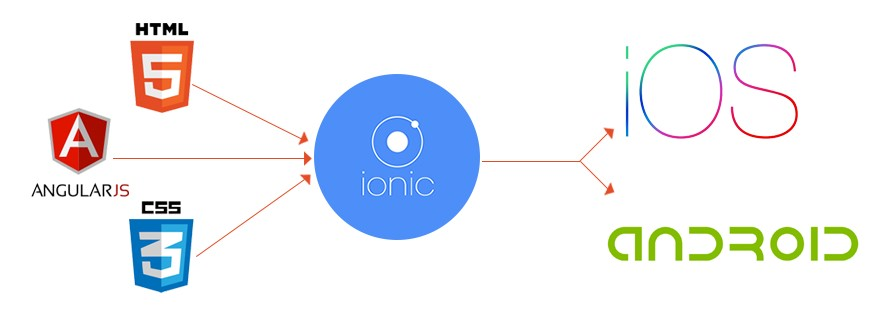
\includegraphics[width=\columnwidth]{Figures/2/ionic-structure}
		\caption{โครงสร้างของ Ionic Framework}
		\label{Fig:ionic-structure}
	\end{figure}
	
	\subsection{รายละเอียดของ Cordova}
		Cordova ถูกพัฒนาจาก Nitobi ในปี ค.ศ.2009 เป็น Open Source ที่ช่วยให้เทคโนโลยีเว็บสามารถใช้งานกับมือถือได้ ซึ่งก่อนหน้ามีชื่อว่า “PhoneGap” และ Cordova เป็นตัวจัดการเทคโนโลยีเว็บให้เข้าถึงการทำงานของระบบปฏิบัติการ เช่น การถ่ายรูป การเรียกไฟล์จากตัวเครื่อง จีพีเอส เป็นต้น ด้วยการทำงานผ่านไลบรารี่ (Library) ซึ่งสามารถใช้ได้ทุกระบบปฏิบัติการทั้ง Window Phone, Blackberry, IOS หรือ Android 

		\begin{figure}[H]
			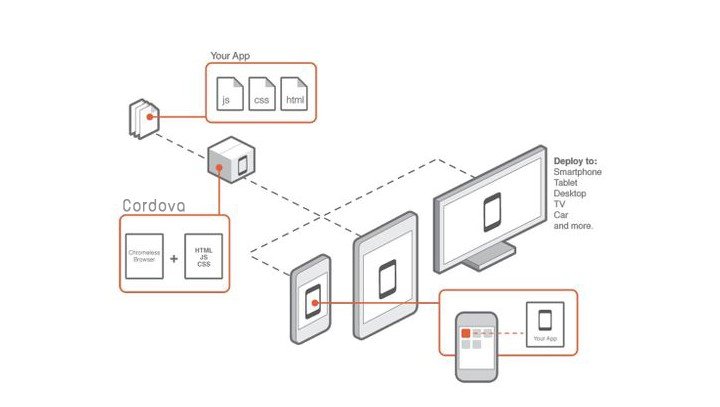
\includegraphics[width=\columnwidth]{Figures/2/cordova-structrue}
			\caption{โครงสร้างของ Cordova}
			\label{Fig:cordova-structrue}
		\end{figure}

	\subsection{Hybrid Mobile Application }
		Ionic Framework เป็นแอปพลิเคชั่นประเภท Hybrid Mobile เป็นการเขียนแอปพลิเคชันระหว่าง Native Application [11] และ Web Application [12] เพื่อแก้ไขปัญหาในการทำงานซ้ำซ้อนระหว่างระบบปฏิบัติการ ซึ่งการเขียนแอพพลิเคชั่นสามารถใช้งานได้กับทุกระบบปฏิบัติการ และยังสามารถเรียกใช้งานทรัพยากรของระบบปฏิบัติการของโทรศัพท์สมาร์ทโฟนนั้นได้อย่างอิสระ

	\subsection{Lifecycle events }
		การเปลี่ยนหน้าเพจของ Ionic framework จะเป็นการสแตก (Stack) ของหน้าเพจ มีคำสั่ง pop สำหรับดึงหน้าเพจออกจากสแตกและคำสั่ง push สำหรับซ้อนทับหน้าเพจใหม่เข้ามาในสแตก
		
		Lifecycle events [10] จะเกิดขึ้นในระหว่างการเปลี่ยนหน้าเพจ 
		การแสดงเพิ่มเข้ามาและการปิดหรือลบออกไปของ Component ที่มีรูปแบบการใช้งานคล้ายเพจ 
		ในบางครั้งการกำหนดการทำงานแทรกเข้าไปในเพจ ดังต่อไปนี้

		\begin{enumerate}
			\item ionViewDidLoad: เริ่มทำงานเมื่อโหลดหน้าเพจและถูกเก็บข้อมูลในหน่วยความจำ กิจกรรมนี้จะไม่เกิดขึ้นเมื่อหน้าเพจมีการแคช (Cache) เกิดขึ้น
			\item ionViewWillEnter: เริ่มทำงานเมื่อหน้าเพจถูกเรียกขึ้นมาแสดงและกลายเป็นหน้าเพจที่ใช้งานอยู่
			\item ionViewDidEnter: เริ่มทำงานเมื่อหน้าเพจที่ใช้งานอยู่ถูกเรียกมาอย่างสมบูรณ์ กิจกรรมนี้จะไม่เกิดขึ้นเมื่อหน้าเพจมีการแคชเกิดขึ้น
			\item ionViewWillLeave: เริ่มทำงานเมื่อกำลังจะออกจากหน้าเพจและไม่ใช่หน้าเพจที่ใช้งานอยู่
			\item ionViewDidLeave: เริ่มทำงานเมื่อออกจากหน้าเพจเสร็จสิ้นแล้วและไม่ใช่หน้าเพจที่ใช้งานอยู่
			\item ionViewWillUnload: เริ่มทำงานเมื่อหน้าเพจนั้นถูกทำลายหรือถูกลบหน้าเพจออกไป
			\item ionViewCanEnter: เริ่มการทำงานก่อนจะโหลดหน้าเพจ ใช้สำหรับกำหนดสิทธิการเข้าไปยังหน้าเพจ
			\item ionViewCanLeave: เริ่มการทำงานก่อนมีการออกจากหน้าเพจ ใช้สำหรับกำหนดเงื่อนไขในการออกจากหน้าเพจ
		\end{enumerate}

	\subsection{ข้อดีและข้อเสียของ Ionic Framework}
		\begin{enumerate}
			\item ข้อดีของ Ionic Framework
			\begin{itemize}
				\item สามารถทำงานใช้งานได้หลายระบบปฏิบัติการ
				\item มีส่วนติดต่อผู้ใช้งาน (User Interface) ที่ถูกออกแบบมาสวยงาม 
				\item ใช้เทคโนโลยี HTML CSS และ JavaScript ที่ได้รับการยอมรับและใช้งานอย่างแพร่หลาย	
			\end{itemize}
			\item ข้อเสียของ Ionic Framwork
				\begin{itemize}
					\item มีข้อจำกัดการทำงานใน WebView [6] ของระบบปฏิบัติการแอนดรอยด์ 4.0 ในการเล่น Animation รวมถึงการทำงานของ JavaScript ค่อนข้างช้า
				\end{itemize}
		\end{enumerate}

\section{ความรู้พื้นฐานเกี่ยวกับภาษา TypeScript}
	TypeScript เป็นภาษาโปรแกรมที่พัฒนาโดย Microsoft



\section{ความรู้พื้นฐานเกี่ยวกับ Docker }
	Docker [9] เป็นซอฟแวร์ Open-source สำหรับสร้างแพ็จเกจของ application ที่เก็บรวมเข้าไว้ด้วยกันใน Container 
	ที่มีการทำงานในลักษณะจำลองสภาพแวดล้อมขึ้นมาบนเครื่องเซิฟเวอร์ 
	เพื่อใช้ในการเริ่มการทำงานของเซอร์วิสที่ต้องการ 
	มีการทำงานคล้ายคลึงกับ Virtual Machine 
	แต่มีข้อแตกต่างกันในการจำลองสภาพแวดล้อมทั้ง OS 
	เพื่อใช้งาน แต่สำหรับ Docker จะใช้ Container ในการจำลองสภาพแวดล้อมขึ้น 
	เพื่อใช้งานสำหรับเซอร์วิสที่ต้องการใช้งานเท่านั้น 
	โดยไม่มีส่วนของ OS เข้าไปเกี่ยวข้องเหมือนกับ Virtual Machine แสดงดังรูปที่ \ref{Fig:containers_vs_VM}
	
	ในการติดตั้งเว็บเซอร์วิสที่เครื่องเซิฟเวอร์ที่มีสภาพแวดล้อมไม่เหมือนกับเครื่องที่ใช้พัฒนา 
	จำเป็นจะต้องติดตั้งส่วนเสริมเพิ่มเติมเข้ามาในเครื่องเซิฟเวอร์อีก และเพื่อป้องกันปัญหานี้ 
	ผู้พัฒนาได้พัฒนาเว็บเซอร์วิสของแอปพลิเคค้นหายาเพื่อคุณไว้ใน 
	Docker image สำหรับพร้อมติดตั้งด้วย Docker Engine  

	\begin{figure}
		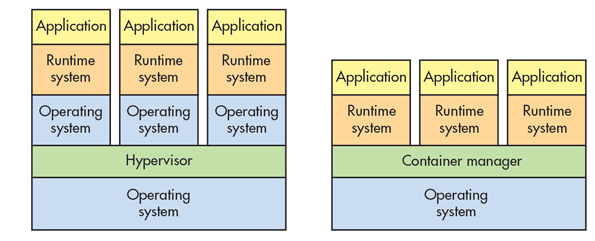
\includegraphics[width=\columnwidth]{Figures/2/containers_vs_VM}
		\caption{ความแตกต่างสถาปัตยกรรมระหว่าง Containers และ Virtual Machines}
		\label{Fig:containers_vs_VM}
	\end{figure}

	\subsection{รายละเอียดของ Docker Concepts}
		\begin{enumerate}
			\item Images เป็นเหมือนกับตัวต้นแบบของ container ภายในประกอบด้วย application ที่มีการติดตั้งเพื่อใช้งานสำหรับเซอร์วิส มีการกำหนดการตั้งค่าไว้เรียบร้อย และนำมาสร้างเป็น docker images เก็บไว้บน docker registry เพื่อนำไปใช้งาน
			\item Container ถูกสร้างมาจาก images และเมื่อสร้างขึ้นมาจะเป็นการเริ่มทำงานของเซอร์วิส ซึ่งภายใน container แต่ละตัวจะมีการใช้งาน RAM CPU และไฟล์ config เป็นต้น เปรียบเสมือนเป็นเครื่องเซิฟเวอร์ผู้ใช้งานสามารถควบคุมและจัดการกับ binaries, dependencies ทั้งหมดได้ใน container
			\item Registries and Repositories เป็นคลาวด์เซิร์ฟเวอร์สำหรับเก็บ image ไว้บน DockerHub [15] และภายใน registry จะมี repositorites ที่เอาไว้จัดเก็บ image ที่อยู่ใน registry
		\end{enumerate}

	\subsection{ข้อดีของ Docker}
		\begin{enumerate}
			\item สามารถใช้งานได้บน Linux Mac และ Windows
			\item มีขนาดข้อมูลเล็กและการติดตั้งได้อย่างเร็วรวด เพราะไม่มีส่วน OS
			\item มีความต้องการในการใช้ CPU RAM และพื้นที่น้อยกว่า Virtual Machine
			\item ลดปัญหาสภาพแวดล้อมที่ต่างกัน ระหว่างติดตั้งที่เครื่องเซิฟเวอร์
			\item ผู้ใช้งานสามารถ pull image จาก docker registry ที่มีการสร้างไว้ให้แล้วมาใช้งาน 
		\end{enumerate}
	\subsection{คำสั่งเบื้องต้น}
		มีคำสั่งเบื้องต้นดังต่อไปนี้
		\begin{enumerate}
			\item docker images แสดงรายการรายละเอียด images ทั้งหมดบนเครื่องผู้ใช้งาน
			\item docker pull คำสั่งดึง images จาก registry มาไว้ที่เครื่องผู้ใช้งาน
			\item docker ps แสดงรายการรายละเอียดของ container ที่กำลังทำงานอยู่ทั้งหมด
			\item docker stop CONTAINER ID คำสั่งหยุดการทำงานของ container 
			\item docker start CONTAINER ID คำสั่งเริ่มการทำงานของ container 
			\item docker rm CONTAINER ID คำสั่งลบ container
			\item docker logs CONTAINER ID คำสั่งเพื่อดูข้อมูลการทำงานของ container
			\item docker run IMAGES NAME ใช้ในการสร้าง container ใหม่ ในกรณีที่ไม่มี images นั้นๆ บนเครื่องผู้ใช้งาน docker จะ pull images มาไว้ที่เครื่องผู้ใช้งานโดยอัตโนมัติ
		\end{enumerate}
	
	\subsection{การใช้งาน Docker ใน Ubuntu}
		การใช้งาน Docker ใน Ubuntu [17] สามารถอธิบายได้ดังรูปที่ \ref{Fig:UsingDocker} ดังต่อไปนี้
		\begin{itemize}[label={--}]
			\item บรรทัดที่ 1 – 2 เป็นการติดตั้ง Docker สามารถเรียกใช้ผ่าน Command line
			\item บรรทัดที่ 3 ทดสอบการทำงานของ Docker ด้วยการเรียกใช้งาน Image ที่ชื่อ “hello-world”
			\item บรรทัดที่ 4 – 8  ถ้าที่เครื่องผู้ใช้งานไม่มี image นั้น Docker จะทำการดาวโหลดจาก Docker Hub มาที่เครื่องผู้ใช้งาน 
			\item บรรทัดที่ 9 Docker สามารถทำงานได้ตามปกติ และเรียกใช้งาน Image hello-world ได้สำเร็จ
		\end{itemize}

		\begin{figure}[H]
			{\setstretch{1.0}\begin{lstlisting}
sudo apt - get update 
sudo apt - get install - y docker - ce   
docker   run hello-world   
Unable  to  find  image  'hello-world:latest'  
locally  latest:  Pulling  from  library  /  hello  -  world  
78445 dd45222: Pull complete Digest: sha256: c5515758d4c5e1e838e9cd307f6c6a0d 620b5e07e6f927b07d05f6d12a1ac8d7  
Status: Downloaded newer image  
for  hello  -  world:  latest  
Hello   from   Docker!This   message   shows   that   your   installation   appears   to   be   working   correctly. 
			\end{lstlisting}}
			\caption{คำสั่งในการใช้งาน Docker}
			\label{Fig:UsingDocker}
		\end{figure}
		

\section{ความรู้พื้นฐานเกี่ยวกับ HTTP Protocol}
	HTTP (Hypertext Transfer Protocol) เป็นโปรโตรคอลที่อยู่ในส่วนของ Application Layer 
	และเป็นโปรโตรคอลสื่อสารสำหรับการแลกเปลี่ยนสารสนเทศอินเทอร์เน็ตของ World Wide Web (WWW) 
	ซึ่งมีโครงสร้างเป็นตัวอักษรและตัวเลข (Text) เรียกว่า ทรัพยากร (Resource) 
	โดยทรัพยากรเป็นข้อมูลต่างๆ เช่น HTML ไฟล์ รูปภาพ และวิดิโอ เป็นต้น
	
	แอปพลิเคชันค้นหายาเพื่อคุณอาศัย HTTP ในการสือสารกับเว็บเซอร์วิส โดยใช้ HTTP Method สำหรับร้องขอทรัพยากร (HTTP Request) จากเว็บเซอร์วิสและคืนทรัพยากร (HTTP Response) จากเว็บเซอร์วิสมายังเครื่องผู้ใช้งาน 

	\subsection{HTTP Method}
		HTTP ได้กำหนดคำสั่งร้องขอไว้ทั้งหมด 8 คำสั่ง แสดงการกระทำที่ต้องการ เพื่อที่จะดำเนินการกับทรัพยากรที่ถูกระบุ ดังต่อไปนี้

		\begin{enumerate}
			\item HEAD ร้องขอการตอบรับจากทรัพยากรที่ระบุ คล้ายกับ GET แต่จะไม่มีส่วนเนื้อหาที่ร้องขอกลับมา คำสั่งนี้ใช้ประโยชน์ในการตรวจสอบข้อมูลส่วนห้วของการตอบรับ โดยไม่จำเป็นต้องส่งเนื้อหาเต็มมาทั้งหมด
			\item GET ร้องขอการนำเสนอจากทรัพยากรที่ระบุและมีส่วนของเนื้อหาที่ร้องขอ
			\item POST ส่งข้อมูลไปยังทรัพยากรที่ระบุเพื่อให้นำไปประมวล
			\item PUT อัปโหลดการนำเสนอของทรัพยากรที่ระบุ
			\item DELETE ลบทรัพยากรที่ระบุ
			\item TRACE ส่งข้อมูลร้องขอกลับมา เครื่องลูกข่ายจะเห็นว่ามีข้อมูลที่สื่อกลางเพิ่มหรือเปลี่ยนแปลงข้อความร้องขอก่อนไปถึงทรัพยากรปลายทาง
			\item OPTIONS คืนค่าเป็นรายชื่อคำสั่ง HTTP ที่เครื่องแม่ข่ายนั้นรองรับสำหรับทรัพยากรที่ระบุ
			\item CONNECT แปลงการเชื่อมต่อของการร้องขอไปเป็น TCP/IP [14]
		\end{enumerate}

	\subsection{รายละเอียดของ HTTP Request}
		รูปแบบโครงสร้างของ HTTP Request เป็นการข้อมูลโดยผู้ใช้งานไปยังเซิฟเวอร์เพื่อให้ส่งข้อมูลตอบกลับมาที่ผู้ใช้งานแสดงดังรูปที่ \ref{Fig:HTTP-request-structrue} และรายละเอียดใน HTTP Request มีดังนี้
	\subsection{รายละเอียดของ HTTP Response}
		\begin{enumerate}
			\item <VERB> เป็นส่วนของ HTTP method 
			\item <URL> เป็นตำแหน่งของสถานที่ข้อมูลที่ต้องการให้ระบบทำงาน
			\item <HTTP Version> เป็นเวอร์ชันของ HTTP
			\item <Request Header> เป็นส่วนของ Metadata ที่ใช้เก็บค่า key-value ของ Header เพื่อบอกข้อมูลผู้ส่ง
			\item <Request Body> เป็นส่วนข้อมูล Content ใน REST
		\end{enumerate}
		\begin{figure}
			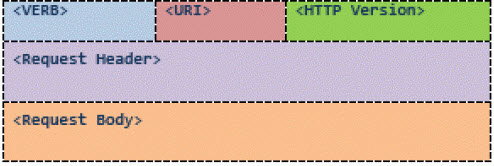
\includegraphics[width=\columnwidth]{Figures/2/HTTP-request-structrue}
			\caption{รูปแบบโครงสร้างของ HTTP Request}
			\label{Fig:HTTP-request-structrue}
		\end{figure}

	\subsection{รายละเอียดของ HTTP Response}
		รูปแบบโครงสร้างของ HTTP Response คือการส่งข้อมูลที่ทางเซิฟเวอร์ตอบรับกลับไปยังผู้ใช้งานตามที่ได้ขอมาแสดงดังรูปที่ \ref{Fig:HTTP-response-structrue} และรายละเอียดใน HTTP Response มีดังนี้

		\begin{enumerate}
			\item <HTTP Version> เป็นเวอร์ชันของ HTTP
			\item <Response Code> เป็นผลลัพธ์การทำงานในระบบ HTTP เป็นตัวเลข 3 หลัก เช่น 2XX การร้องขอสำเร็จ, 3XX การเปลี่ยนทาง, 4XX ความผิดพลาดจากเครื่องผู้ใช้งาน, 5XX ความผิดพลาดจากเครื่องเซิฟเวอร์
			\item <Request Body> เป็นส่วนข้อมูลผลลัพธ์ Content ใน REST ที่เซิฟเวอร์ตอบกลับมาที่ผู้ใช้งาน
		\end{enumerate}
		\begin{figure}
			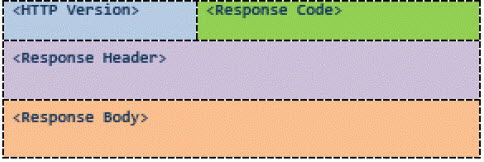
\includegraphics[width=\columnwidth]{Figures/2/HTTP-response-structrue}
			\caption{รูปแบบโครงสร้างของ HTTP response}
			\label{Fig:HTTP-response-structrue}
		\end{figure}

\section{ความรู้พื้นฐานเกี่ยวกับ RESTful API}
	REST (Representational state transfer) คือการสร้างเว็บเซอร์วิสชนิดหนึ่งที่อาศัย HTTP Method GET, POST, PUT และ DELETE ในการทำงาน ใช้หลักการแบบ stateless คือไม่มีการใช้งาน session และส่งผลกลับมาในรูปแบบของ JSON หรือ XML มีขนาดข้อมูลที่เล็ก สามารถส่งผลให้สามารถรับส่งข้อมูลไปมาข้าม Platform ได้อย่างสะดวก เนื่องจากเป็นการเรียกใช้งานผ่าน HTTP Protocol ที่ใช้ในการเรียกเว็บไซต์ จึงเป็นที่นิยม และแอปพลิเคชันค้นหายาเพื่อคุณกับเว็บเซอร์วิสติดต่อสื่อสารผ่าน HTTP โดยใช้ HTTP method ในการร้องขอทรัพยากรจากเว็บเซอร์วิสและส่งทรัพยากรกลับมาที่แอปพลิเคชันในรูปแบบของ JSON ดังแสดงในรูปที่ 
	\ref{fig:format-JSON}  

	\begin{figure}
		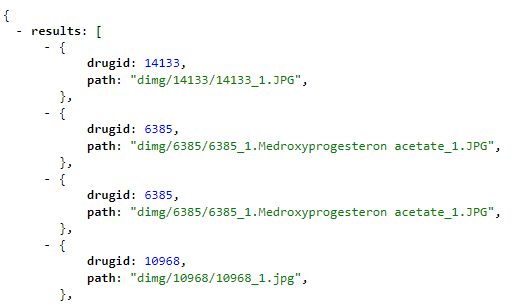
\includegraphics[width=\columnwidth]{Figures/2/format-JSON}
		\caption{ตัวอย่างรูปแบบของ JSON}
		\label{fig:format-JSON}
	\end{figure}

\section{การทำ Authentication ด้วย JSON Web Token }
	\subsection{การพิสูจน์ตัวตน (Authentication)}
		ในบางแอพพลิเคชั่นจะสามารถใช้งานได้จำเป็นต้องรู้จักผู้ใช้งานที่กำลังใช้งานอยู่ ซึ่งระบบที่ทำหน้าที่ในการตรวจสอบ เรียกว่า “Authentication” 
	
		ผู้พัฒนาได้พัฒนาการพิสูจน์ตัวตนก่อนใช้งานเว็บเซอร์วิสด้วย JSON Web Token [1] เพื่อป้องการเข้าถึงข้อมูลจากผู้ที่ไม่พึ่งประสงค์ โดยการร้องขอทรัพยากรไปยังเว็บเซอร์วิสจากแอปพลิเคชันค้นหายาเพื่อคุณ จะฝั่ง JSON Web Token ไว้ใน Header ของ HTTP Requset เพื่อไว้สำหรับการพิสูจน์ตัวตนของเว็บเซอร์วิส และรายละเอียดของ JSON Web Token มีดังนี้ 
	
	\subsection{รายละเอียดของ JSON Web Token (JWT) }
		JSON Web Token เป็นมาตรฐานเปิด (RFC 7519) ที่เข้ามาแก้ปัญหาการส่งข้อมูลอย่างปลอดภัยระหว่างแอพพลิเคชั่นและเว็บเซอร์วิส โดยถูกออกแบบให้มีขนาดที่กระทัดรัด (Compact) และเก็บข้อมูลภายในตัว (Self-contained) JWT เป็น Token หรือ ชุดตัวอักษร โดยมีโครงสร้างแบ่งออกเป็น 3 ส่วน ได้แก่
		\begin{enumerate}
			\item Header สำหรับเก็บประเภทการเข้ารหัสของโทเคน 
			\item Payload สำหรับเก็บข้อมูล
			\item Signature ส่วน Digital Signed ซึ่งเหมือนกับลายเซ็นทิ้งท้ายไว้ตรวจสอบว่าเป็นโทเคนที่ถูกสร้างอย่างถูกต้องหรือไม่ถูกต้อง และถ้าหากมีผู้เขียนแปลงข้อมูลของโทเคนจะทำให้การตรวจสอบ Signature ไม่ถูกต้อง 
		\end{enumerate}
		\begin{figure}
			
\includegraphics[width=\columnwidth]{Figures/2/JWT-structure}
			\caption{ตัวอย่างรูปแบบของ JSON Web Token}
			\label{fig:JWT-structure}
		\end{figure}

	\subsection{การใช้งาน JSON Web Token}
	ผู้พัฒนาเลือกพัฒนา JWT ด้วย Node.js ที่มีแพ็กเกจรองรับการใช้งาน JWT
	\begin{enumerate}
		\item การสร้าง JSON Web Token
		จากรูปที่ \ref{Fig:SignJWT} สามารถอธิบายได้ดังนี้
		\begin{itemize}
			\item บรรทัดที่ 1 เรียกแพ็กเกจ jsonwebtoken มาเก็บที่ตัวแปร jwt
			\item บรรทัดที่ 2 เรียกใช้งานฟังก์ชัน sign สำหรับการสร้าง JSON WebToken โดยกำหนดให้ data คือ“foobar” คำลับ คือ “secret” และเวลาหมดอายุของ Token คือ 1 ชั่วโมง
		\end{itemize}
		\begin{figure}[H]
			{\setstretch{1.0}\begin{lstlisting}
var  jwt  =  require('jsonwebtoken');  
var  token  =  jwt.sign({  
	data: 'foobar'  
}, 'secret', {  
	expiresIn: '1h'  
});  
			\end{lstlisting}}
			\caption{ตัวอย่างการสร้าง JSON Web Token}
			\label{Fig:SignJWT}
		\end{figure}

		\item การตรวจสอบ JSON Web Token
			ในการตรวจสอบความถูกต้องของโทเคน คำลับในการสร้างและการตรวจสอบต้องเหมือนกัน 
			โทเคนจะต้องไม่หมดอายุและโทเคนจะต้องไม่ถูกเปลี่ยนตัวอักษร
			จากรูปที่ \ref{Fig:VerifyJWT} สามารถอธิบายได้ดังนี้
			\begin{itemize}
				\item บรรทัดที่ 1 เรียกใช้งานฟังก์ชัน verify สำหรับตรวจสอบความถูกต้องของ token โดยกำหนดคำลับ คือ ‘secret’ 
				\item บรรทัดที่ 2 เมื่อการตรวจสอบ token เสร็จแล้ว จะได้ผลลัพธ์ในตัวแปรชื่อว่า decoded ถ้าหากการตรวจสอบถูกต้องตัวแปร err จะมีค่าเป็น null และถ้าหากการตรวจสอบไม่ถูกต้องตัวแปร err มีค่าเป็นข้อความผิดพลาดจากการตรวจสอบ
			\end{itemize}
			\begin{figure}[H]
				{\setstretch{1.0}\begin{lstlisting}
jwt.verify(token,  'secret',  function(err,  decoded)  {  
	console.log(decoded)  
});  
				\end{lstlisting}}
				\caption{ตัวอย่างการตรวจสอบ JSON Web Token}
				\label{Fig:VerifyJWT}
			\end{figure}
	\end{enumerate}
	
	\subsection{ข้อดีและข้อเสียของ JWT}
		\begin{enumerate}
			\item ข้อดีของใช้งาน JWT สำหรับการ Authentication
			\begin{itemize}
				\item JWT สามารถใช้งานได้กับทุกภาษาที่รองรับข้อมูลแบบ JSON 
				\item สามารถส่ง JWT ผ่าน HTTP ใน Header POST และ URL ได้ง่าย รวดเร็ว
				\item มีความปลอดภัยในตัวของมันเอง 
			\end{itemize}
			\item ข้อเสียของใช้งาน JWT สำหรับการ Authentication 
			\begin{itemize}
				\item JWT สามารถเก็บข้อมูลในตัวเอง แต่ข้อมูลนั้นต้องเป็นข้อมูลที่สามารถเปิดเผยได้
				\item ถ้าหาก JWT ถูกขโมยไปใช้กับเว็บเซอร์วิส ก็จะสามารถทำ Authentication API ได้
				\item ข้อมูลที่ถูกเก็บไว้ใน JWT จะไม่สามารถถูกอัพเดทข้อมูลได้
			\end{itemize}
		\end{enumerate}
		
			
\section{ความรู้พื้นฐานเกี่ยวกับ OpenCV (Open Source Computer Vision) }
	OpenCV เป็นไลบรารี่ (Library) ที่รวบรวมฟังก์ชั่นสำหรับการประมวลผลภาพและคอมพิวเตอร์วิทัศนศาสตร์ไว้เป็นจำนวนมาก อยู่ภายใต้ใบอนุญาติ BSD ซึ่งสามารถใช้ได้ฟรีทั้งทางด้านการศึกษาและทางการค้า เนื่องจากนี้ยังมีการประยุกต์ใช้งาน OpenCV ในแบบต่างๆ ได้แก่ ระบบตรวจจับใบหน้า (Face Detection) การจดจำใบหน้า (Face Recognition) การติดตามวัถตุ (Object Tracking) การเรียนรู้ของเครื่อง (Machine Learning) เป็นต้น
	\subsection{การประมวลผลภาพ (Image Processing)}
	การประมวลผลภาพคือการนำรูปที่มีอยู่แล้ว หรือรูปที่รับเข้ามาจากอุปกรณ์ต่างๆ 
	หรือรูปที่มีอยู่มาประมวลผลเพื่อหาลักษณะเด่นบางประการของรูปที่มีอยู่ 
	หรืออาจจะเป็นการตีความหมายของภาพ รวมถึงการปรับคุณลักษณะของภาพให้เป็นไปตามต้องการ 
	โดยใช้กระบวนการทางคณิตศาสตร์
	
	การประมวลผลภาพแนวคิดทางคณิตศาสตร์ที่ใช้ในการประมวลผล Signal processing 
	มาทำการประยุกต์ใช้กับสัญญาณภาพ และภาพจะเก็บอยู่ในรูปของอาเรย์ (Array) 
	โดยกลุ่มของของอาเรย์กลุ่มหนึ่งจะเป็นค่าของภาพหนึ่งพิกเซล 
	เช่น ภาพแบบ RBG ใช้อาเรย์ 3 ช่องเพื่อเก็บค่าสีของ RBG ในหนึ่งพิกเซล รูปแบบการจัดเก็บภาพแต่ละชนิดจะแตกต่างกัน 
	ขึ้นอยู่กับระบบสีของภาพ โดยแบ่งชนิดของภาพได้ดังนี้
	\begin{itemize}
		\item Binary Image เป็นรูปที่มีสีเพียงสองระดับคือสีขาวและสีดำ 
		โดยในอาเรย์ช่องนั้นมีค่าคือ 0 หมายความว่าดำ และ 255 หมายความว่าขาว
		ดังรูปที่ \ref{Fig:binary-image }
		\begin{figure}[H]
			\centering
			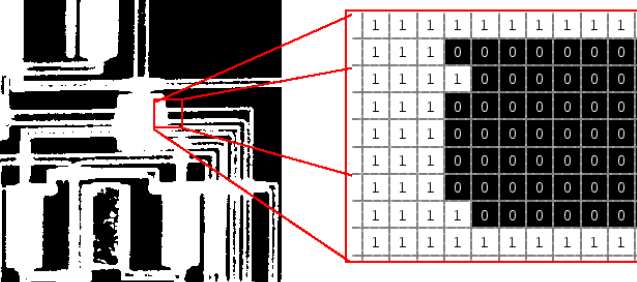
\includegraphics[scale=0.7]{Figures/2/binary-image}
			\caption{ภาพแบบ Binary }
			\label{Fig:binary-image }
		\end{figure}
		
		\item Grayscale Image เป็นรูปที่มี channel เดียว 
		โดยเก็บเป็นอาเรย์คล้ายกับภาพ Binary Image 
		แต่ค่าที่อยู่ในอาเรย์เป็นค่าความสว่าง ซึ่งมีค่าได้ตั้งงแต่ 0 ถึง 255
		ดังรูปที่ \ref{Fig:grayscale-image }
		\begin{figure}[H]
			\centering
			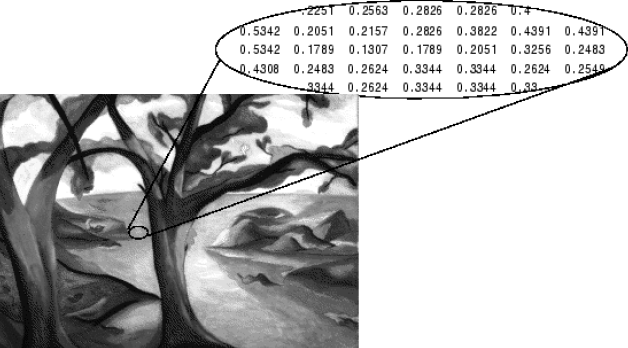
\includegraphics[scale=0.7]{Figures/2/grayscale-image}
			\caption{ ภาพแบบ Grayscale }
			\label{Fig:grayscale-image }
		\end{figure}
		
		\item RGB Image เป็นรูปที่มี 3 channel 
		โดยภาพจะเก็บอยู่ในรูปภาพโดเรียงตามลำดับ BGR 
		แต่ถ้าอยู่ในไฟล์ภาพจะเรียงตามปกติ คือ RBG 
		ดังรูปที่ \ref{Fig:rbg-image }
		\begin{figure}[H]
			\centering
			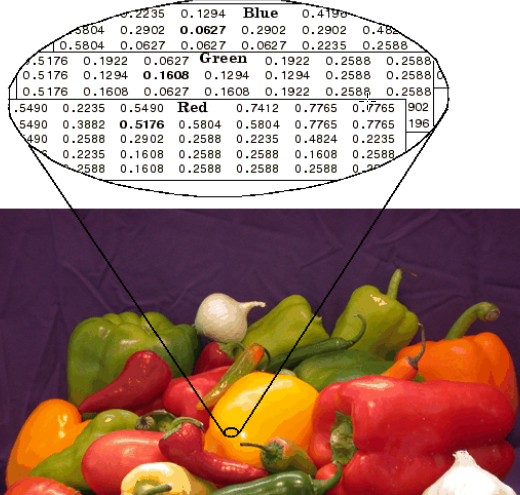
\includegraphics[scale=0.7]{Figures/2/rbg-image}
			\caption{ภาพแบบ RBG }
			\label{Fig:rbg-image }
		\end{figure}
	\end{itemize}

	\subsection{การทำ Thresholding รูปภาพ}
		การทำ Thresholding เป็นวิธีการแยกบริเวณรูปภาพ (Image Segmentation) ของภาพสีเทา (Grayscale) 
		จากรูปที่ \ref{Fig:thresholding} ผู้พัฒนากำหนดค่า threshold เท่ากับ 120 
		ในรูปภาพค่าพิกเซลแต่ละพิกเซลของภาพต้นฉบับที่มีค่าน้อยกว่า 120 
		จะถูกกำหนดเป็นค่าพิกเซลของภาพผลลัพธ์เป็น 0 (สีขาว) และถ้าในรูปภาพค่าพิกเซลแต่ละพิกเซลของภาพต้นฉบับนั้นมีค่ามากกว่าเท่ากับ 120 จะถูกกำหนดพิกเซลของภาพผลลัพต์เป็น 255 (สีดำ) จะได้สมการดังรูปที่  เมื่อ f(x, y) คือ ตำแหน่งพิกเซลของภาพต้นฉบับ และ g(x, y) คือ ตำแหน่งพิกเซลของภาพผลลัพธ์

		ตัวอย่างการทำ Thresholding ได้แก่การรูปภาพต้นฉบับนำมาเข้าสมการตามรูปที่ \ref{Fig:thresholding-example} และกำหนดค่า threshold เท่ากับ 120 ดังนั้นผลลัพธ์จะได้ดังรูปที่ \ref{Fig:thresholding-result}
		
		\begin{figure}[H]	
			\centering			
			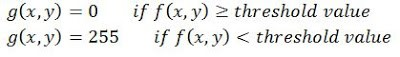
\includegraphics[scale=1]{Figures/2/thresholding}
			\caption{สมการการทำ Thresholding รูปภาพ}
			\label{Fig:thresholding}
		\end{figure}
		
		\begin{figure}[H]	
			\centering			
			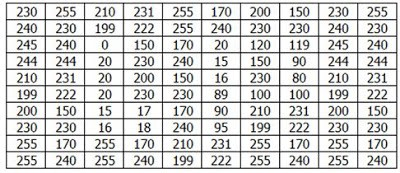
\includegraphics[scale=1]{Figures/2/thresholding-example}
			\caption{ตัวอย่างการทำ Thresholding รูปภาพต้นฉบับขนาด 10x10 พิกเซล}
			\label{Fig:thresholding-example}
		\end{figure}

		\begin{figure}[H]
			\centering					
			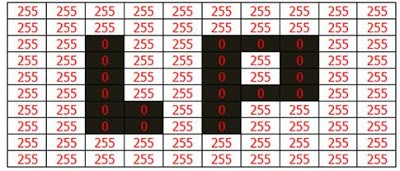
\includegraphics[scale=1]{Figures/2/thresholding-result}
			\caption{ตัวอย่างการทำ Thresholding รูปภาพผลลัพธ์ขนาด 10x10 พิกเซล}
			\label{Fig:thresholding-result}
		\end{figure}

	\subsection{การตรวจหา Canny Edge}
		การหาขอบภาพเป็นการหาเส้นรอบวัถตุที่อยู่ในภาพ เมื่อทราบเส้นรอบวัตถุจะสามารถคำนวณหาพื้นที่หรือจำแนกชนิดของวัถตุนั้นได้ ขอบภาพเกิดจากความแตกต่างของความเข้มแสงจากจุดหนึ่งไปยังอีกจุดหนึ่ง การตรวจหา Canny Edge [5] เป็นอัลกอริทึมการตรวจหาขอบที่เป็นที่นิยม ได้รับการพัฒนาโดย John F. Canny เป็นอัลกอริทึมแบบหลายขั้นตอนและจะดำเนินการผ่านแต่ละขั้นตอน
		\subsubsection{ลดสัญญาณรบกวน (Noise Reduction)} 
		เนื่องจากการตรวจหาขอบมีความอ่อนไหวต่อสัญญาณรบกวนในภาพ ขั้นตอนแรกคือการขจัดสัญญาณรบกวนด้วยตัวกรองแบบเกาส์ (Gaussian) 5x5 
		\subsubsection{การหาการไล่ระดับสีความเข้มของภาพ (Gradient)}
		รูปที่ Smoothing จะถูกกรองด้วย Sobel kernel ทั้งในแนวนอนและแนวตั้งจากจุดหนึ่งไปยังอีกจุด โดยการหาจุดในแนวนอน (Gx) และในแนวตั้ง (Gy) จากทั้งสอง ภาพนี้สามารถหาการไล่ระดับสีและทิศทางของขอบสำหรับแต่ละพิกเซล
		\subsubsection{Nonmaxima Suppression}
		หลังจากที่ผ่านขั้นตอนแรกมาแล้ว รูปที่ได้อาจจะมีเส้นขอบที่ไม่ใช่ขอบที่แท้จริงปรากฏอยู่ เนื่องจากสัญญาณรบกวนหรือลักษณะของวัตถุในภาพเป็นพื้นผิวที่มีลวดลายหรือมีรายละเอียดภายในมาก ดังนั้นเพื่อลดปัญหาดังกล่าวจึงได้มีการกำหนดค่า threshold ขึ้นมา 2 ค่า คือ High threshold (T1) และ Low threshold (T2) โดยพิกเซลที่มีค่ามากกว่า T1 จะถูกปรับเป็น 1 (ให้เป็นพิกเซลที่เป็นขอบ) แต่ถ้าน้อยกว่า T2 จะถูกปรับเป็น 0 ส่วนค่าที่อยู่ระหว่างค่า threshold ทั้งสอง การปรับเป็นค่า 0 หรือ 1 ขึ้นอยู่กับพิกเซลที่อยู่รอบข้าง หากพบว่าพิกเซลที่อยู่รอบข้างของพิกเซลที่เป็นขอบมีค่ามากกว่า T2 แล้ว จะปรับค่าพิกเซลดังกล่างให้มีค่าเป็น 1 และถือเป็นสมาชิกหนึ่งในภาพขอบด้วย
		\begin{figure}[H]
			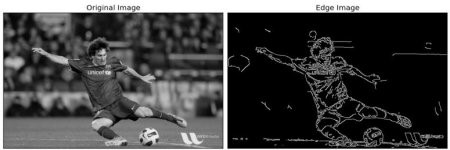
\includegraphics[width=\columnwidth]{Figures/2/canny-edge-detected}
			\caption{ตัวอย่างการตราจหา Canny Edge}
			\label{Fig:canny-edge-detected}
		\end{figure}


	\subsection{การหา Contour Approximation}
		\vspace{-5mm}

		รูปทรง (Contours) สามารถอธิบายได้ง่ายๆว่าเป็นเส้นโค้งที่เชื่อมต่อกับจุดต่อเนื่องทั้งหมดตามแนวขอบที่มีสีเดียวกัน และรูปทรงเป็นเครื่องมือที่มีประโยชน์สำหรับการวิเคราะห์รูปทรง การตรวจจับวัถตุและการจดจำ
		\vspace{-5mm}
		
		การใช้ภาพไบนารีจะได้ผลลัพธ์ที่มีความถูกต้องที่ดีกว่า ดังนั้นก่อนที่จะหารูปทรงควรใช้ threshold และ canny edge จากภาพก่อน ใน OpenCV การหารูปทรงคือการหาวัตถุสีขาวจากพื้นหลังสีดำ ดังนั้นวัถตุที่จะตรวจจับควรเป็นสีขาวและพื้นหลังควรเป็นสีดำ
		
		\begin{figure}[H]
			{\setstretch{1.0}\begin{lstlisting}
import  numpy  as  np  2   
import  cv2  im  =  cv2.imread('test.jpg')  
imgray  =  cv2.cvtColor(im,  cv2.COLOR_BGR2GRAY)  
ret,  thresh  =  cv2.threshold(imgray,  127,  255,  0)  
im2,  contours,  hierarchy  =  cv2.findContours(thresh,  cv2.RETR_TREE,  cv2.CHAIN_APPROX_NONE)  
			\end{lstlisting}}
			\caption{ตัวอย่างการใช้งานฟังก์ชัน cv2.findContours() โดยกำหนดค่าพารามิเตอร์เป็น cv2.CHAIN{\_}APPROW{\_}NONE}
			\label{Fig:finContoursNONE}
		\end{figure}
		\begin{figure}[H]
			{\setstretch{1.0}\begin{lstlisting}
import  numpy  as  np  2   
import  cv2  im  =  cv2.imread('test.jpg')  
imgray  =  cv2.cvtColor(im,  cv2.COLOR_BGR2GRAY)  
ret,  thresh  =  cv2.threshold(imgray,  127,  255,  0)  
im2,  contours,  hierarchy  =  cv2.findContours(thresh,  cv2.RETR_TREE,  cv2.CHAIN_APPROX_SIMPLE)  
			\end{lstlisting}}
			\caption{ตัวอย่างการใช้งานฟังก์ชัน cv2.findContours() โดยกำหนดค่าพารามิเตอร์เป็น cv2.CHAIN{\_}APPROW{\_}SIMPLE }
			\label{Fig:finContoursSIMPLE}
		\end{figure}
		
		จากรูปที่ \ref{Fig:finContoursNONE} ในการใช้ฟังก์ชัน cv2.findContours() 
		โดยกำหนดค่าพารามิเตอร์เป็น cv2.CHAIN{\_}APPROX{\_}NONE} จุดขอบทั้งหมดจะทุกเก็บไว้ 
		ซึ่งแตกต่างจากรูปที่ \ref{Fig:finContoursSIMPLE} ที่กำหนดค่าพารามิเตอร์เป็น cv2.CHAIN{\_}APPROW{\_}SIMPLE 
		จะทำการลบจุดที่ซ้ำซ้อนทั้งหมดและบีบอัดเส้นขอบทำให้ประหยัดหน่วยความจำ 
		และจากรูปที่ \ref{Fig:chain_approx_none_vs_simple} รูปสี่เหลี่ยมผืนผ้าแสดงให้เห็นถึงเทคนิคนี้ 
		เพียงวาดจุดบนพิกัดทั้งหมดในอาร์เรย์เส้น (เส้นสีน้ำเงิน)
		
		จากรูปที่ \ref{Fig:chain_approx_none_vs_simple} ภาพด้านซ้ายกำหนดค่าพารามิเตอร์เป็น 
		cv2.CHAIN{\_}APPROW{\_}NONE  ได้ทั้งหมด 734 จุด 
		และภาพด้านขวากำหนดค่าพารามิเตอร์เป็น cv2.CHAIN{\_}APPROW{\_}SIMPLE 
		ได้ทั้งหมด 4 จุด นั้นเป็นเหตุผลที่ผู้พัฒนาจะเลือกใช้ 
		cv2.CHAIN{\_}APPROW{\_}SIMPLE แทน cv2.CHAIN{\_}APPROW{\_}NONE เพื่อความประหยัดหน่วยความจำ

		\begin{figure}[H]
			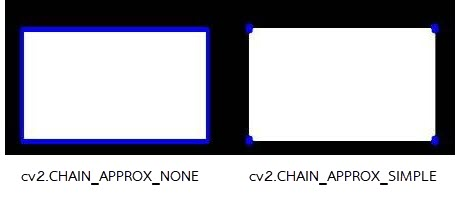
\includegraphics[width=\columnwidth]{Figures/2/chain_approx_none_vs_simple}
			\caption{ผลลัพธ์ของการหา Contours}
			\label{Fig:chain_approx_none_vs_simple}
		\end{figure}
	
	
	\subsection{Support Vector Machines (SVM)}
	SVM เป็นอัลกอริทึมในการคัดแยกที่มีการนำมาใช้กันในด้านการประมวลผลเป็นดิจิตอล 
	หลักการของ SVM คือการให้อินพุทที่ใช้ฝึกเป็นเวคเตอร์ในสเปซ N มิติ เช่นถ้าในกรณีของ 2 มิติ และ 3 มิติ 
	จะเป็นจุดที่อยู่ในระนาบ XY และ XYZ ตามลำดับ จากนั้นทำการสร้างไฮเปอร์เพลน (Hyperplane) 
	ที่จะแยกกลุ่มของเวคเตอร์อินพุทออกเป็นประเภทต่างๆ ในกรณีที่เป็น 2 มิติและ 3 มิติ ไฮเปอร์เพลน คือเส้นตรงและระนาบ 
	
	\begin{figure}[H]
		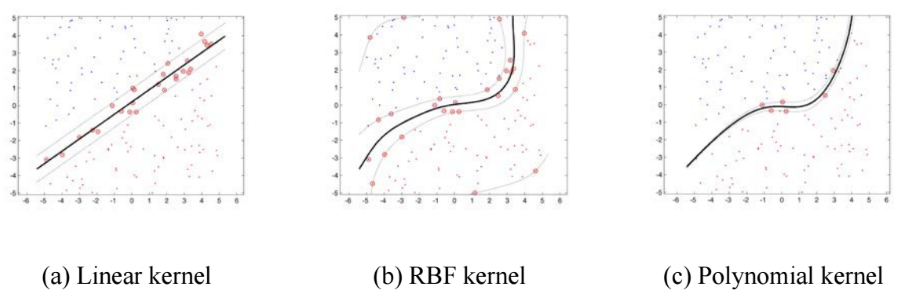
\includegraphics[width=\columnwidth]{Figures/2/format-kernel-function}
		\caption{รูปแบบ kernel function ในแบบต่างๆ}
		\label{Fig:format-kernel-function}
	\end{figure}

	ไฮเปอร์เพลนที่ได้จากการเลือกใช้ kernel function ที่ต่างกันก็จะให้ประสิทธืภาพการทำงานของโมเดลที่ต่างกัน นอกจาการเลือกใช้ kernel function ที่เหมาะสมแล้ว การกำหนดค่าต่างๆ (initial parameters) ของ kernel function ก็มีผลด้วยเช่นกันจากไฮเปอร์เพลนที่แสดงในรูปข้างบนเกิดจากการกำหนดค่าของ initial parameter ที่ต่างกันดังรูปที่ \ref{Fig:format-kernel-function}


	\subsection{K-Nearest Neighbour Algorithm }
	K-Nearest Neighbour Algorithm (KNN) [18] เป็นวิธีที่ใช้ในการจัดแบ่งคลาส (Classification) มีลักษณะการทำงานแบบ Supervised learing (ข้อมูลที่นำมาเรียนรู้ต้องมีคลาสกำกับไว้แล้ว) โดยเทคนิคนี้จะตัดสินใจว่า คลาสใดที่จะแทนเงื่อนไขหรือกรณีใหม่ๆ ได้บ้าง โดยการตรวจสอบจำนวนบางจำนวน (“K” ในขั้นตอนวิธีการ kNN) ของกรณีหรือเงื่อนไขที่เหมือนกันหรือใกล้เคียงกันมากที่สุด โดยจะหาผลรวม (Count Up) ของจำนวนเงื่อนไข หรือกรณีต่างๆ สำหรับแต่ละคลาส และกำหนดเงื่อนไขใหม่ๆ ให้คลาสที่เหมือนกันกับคลาสที่ใกล้เคียงกันมากที่สุด
	
	\subsubsection{ขั้นตอนวิธีการดำเนินการของอัลกอริทึมแบบ K-Nearest Neighbour Algorithm มีดังนี้}
	\begin{enumerate}
		\item กำหนดขนาดของค่า K 
		\item คำนวณระยะห่าง (Distance) ของข้อมูลที่ต้องการพิจารณากับกลุ่มข้อมูลตัวอย่าง
		\item จัดเรียงลำดับของระยะห่าง และเลือกพิจารณาชุดข้อมูลที่ใกล้จุดที่ต้องการพิจารณาตามจำนวนของค่า K ที่กำหนดไว้
		\item พิจารณาข้อมูลจำนวน K ชุด และสังเกตกลุ่มคลาสที่มีจุดใกล้กับจุดพิจารณาเป็นจำนวนมากที่สุด
		\item กำหนดคลาสให้กับจุดพิจารณาที่ใกล้จุดพิจารณมากที่สุด
	\end{enumerate}

	\subsubsection{การดำเนินการหลักของอัลกอริทึมแบบ K-Nearest Neighbour Algorithm ประกอบไปด้วยการทำงาน 2 ฟังก์ชัน ได้แก่}

	\begin{enumerate}
		\item ฟังก์ชันระยะทาง (Distance Function) เป็นการคำนวณค่าระยะห่างระหว่างสองจุด เพื่อที่นำมาวัดความคล้ายคลึงของข้อมูล
		\item ฟังก์ชันการแจกแจง (Combination Function) เป็นการรวมกันของผลลัพธ์ที่ได้จากการคำนวณค่าระยะห่างโดยทำการเรียงลำดับค่าระยะห่างจากน้อยไปมาก จากนั้นนำมาเปรียบเทียบกับค่า K เพื่อหาคลาสของเป้าหมาย
	\end{enumerate}

	\subsection{Random Forest Classifier }
	Random Forest Classifier (RFC) [19] เป็นวิธีที่ใช้ในการจัดแบ่งคลาส โดยหลักการสุ่มข้อมูล (Random sampling) เพื่อสร้างต้นไม้ตัดสินใจขึ้นมาจำนวนมาก ในการจำแนกคลาสของวัถตุโดยจะอินพุทข้อมูลเวกเตอร์ (Vecter) ใส่ให้แต่ละต้นไม้ตัดสินใจที่ถูกสร้างขึ้นมา ต้นไม้แต่ละต้นจะให้คะแนนสำหรับข้อมูลเวกเตอร์ที่ถูกป้อนเข้ามาในแต่ละคลาส วิธีการ Random Forest จะเลือกคลาสที่มีคะแนนมากที่สุดและทำนายคลาสของวัถตุ


\section{การหาขนาดของยาด้วยการใช้วัถตุอ้างอิง}
	การหาขนาดยาด้วยการใช้วัถตุอ้างอิง ด้วยวิธีการเทียบบัญญติไตรยางศ์ [20] เนื่องจากรูปภาพมีหน่วยเป็นพิกเซลและรู้ขนาดด้านยาวและกว้างของวัถตุอ้างอิงแล้ว ถ้าหากวัตถุอ้างอิงมีขนาดด้านยาวเท่ากับ 15 เซนติเมตร ขนาดด้านกว้างเท่ากับ 10 เซนติเมตร และวัตถุอ้างอิงในรูปที่ตรวจจับได้ด้วยการหา Contours ได้ขนาดด้านยาวเท่ากับ 98 พิกเซล ขนาดด้านยาวเท่ากับ 65 พิกเซล และขนาด 1 พิกเซล จะเท่ากับกี่เซนติเมตร ด้วยการเทียบบัญญติไตรยางศ์ จะได้ว่า 15 (เซนติเมตร) / 98 (พิกเซล) เท่ากับอัตราส่วน 0.153 เซนติเมตร/พิกเซล ดังนั้น 1 พิกเซล จะเท่ากับ 0.153 เซนติเมตร และสามารถหาขนาดของยาด้วยการนำ 0.153 ไปคูณกับขนาดพิกเซลของรูปภาพยา

\section{เครื่องมือที่ใช้ในการพัฒนา}
	Nginx [8] มาจากคำว่า “Engine-X” เป็นเว็บเซิร์ฟเวอร์ที่มีประสิทธีภาพดีและนิยมอยู่ในปัจจุบัน ถูกคิดค้นขึ้นมาเพื่อให้สามารถที่จะรองรับการทำงานได้มากกว่า Apache[6] และนอกจากนี้ Nginx ยังมีโมดูลเสริมเข้ามาที่เพียงพอต่อการใช้งานทั่วไป และเป็นซอฟแวร์แบบ Open Source ที่สามารถใช้งานได้ฟรีโดยรองรับระบบปฏิบัติการ Linux และ ระบบปฏิบัติการ Windows
	
	MySQL [7] เป็นโปรแกรมจัดการฐานข้อมูลที่รองรับคำสั่ง SQL เป็นเครื่องมือสำหรับเก็บข้อมูล ที่ต้องใช้ร่วมกับเครื่องมือหรือโปรแกรมอื่นอย่างบูรณาการ เพื่อให้ได้ระบบงานที่รองรับความต้องการของผู้ใช้ เป็นฐานข้อมูลเชิงสัมพันธ์ (RDBMS) ผู้พัฒนาได้นำมาใช้งานกับเว็บเซอร์วิสในการจัดเก็บฐานข้อมูลการพิสูจน์เอกลักษณ์ยาเม็ดหรือแคปซูล
	
	Express – Node.js [3] ถูกสร้างขึ้นบนฐานของระบบ Node.js ซึ่งมีความเร็วของการทำงานและมีความครบถ้วนของระบบ ครอบคลุมในส่วนของการทำงานพื้นฐานในการทำเว็บเซอร์วิส ใช้ในการทำ routing[2] middleware การจัดการ request และ response ทื่ถูกส่งมาจากแอปพลิเคชัน


\chapter{การวิเคราะห์และออกแบบระบบ}

การวิเคราะห์และการออกแบบแอปพลิเคชันค้นหายาเพื่อคุณ เนื่องจากคณะเภสัชศาสตร์ได้สร้างฐานข้อมูลพิสูจน์เอกลักษณ์ยาเม็ดและแคปซูลในประเทศไว้เรียบร้อย ทางผู้พัฒนาจึงได้ดำเนินการเขียนเว็บเซอร์วิส ใช้สำหรับติดต่อฐานข้อมูลพิสูจน์เอกลักษณ์ยาเม็ดและแคปซูลของคณะเภสัชศาสตร์เพื่อดึงข้อมูลพิสูจน์เอกลักษณ์ยาเม็ดและแคปซูลส่งออกให้แอปพลิเคชันในรูปแบบ JSON และการแผนภาพในการออกแบบระบบมีดังนี้ 
\begin{itemize}[label={--}]
	\item รายละเอียดการออกแบบแอปพลิเคชัน
	\item Use Case Diagram เป็นแผนภาพที่ใช้แสดงให้ทราบว่าระบบทำงานหรือมีหน้าที่ใดบ้าง
	\item Class Diagram เป็นแผนภาพที่ใช้แสดง Class และความสัมพันธ์ระหว่าง Class
	\item Sequence Diagram เป็นแผนภาพที่ใช้แสดงให้เห็นถึงการตอบโต้ข้อมูลระหว่างคลาส เรียงตามลำดับของเวลาที่เกิดเหตุการณ์จากน้อยไปมาก
	\item State Diagram ใช้เพื่อแสดงสถานะของวัตถุ รวมไปถึงเหตุการณ์ในแอปพลิเคชัน
	\item การประมวลผลภาพยาเม็ดเพื่อการพิสูจน์เอกลักษณ์ยาเม็ด
\end{itemize}	

\section{รายละเอียดการออกแบบแอปพลิเคชัน}
	โครงงานแอปพลิเคชันค้นหายาเพื่อคุณ Drugiden แบ่งส่วนการทำงานออกเป็น 2 ส่วนหลัก ได้แก่ ส่วนแอปพลิเคชัน และส่วนเว็บเซอร์วิส
	\begin{figure}
		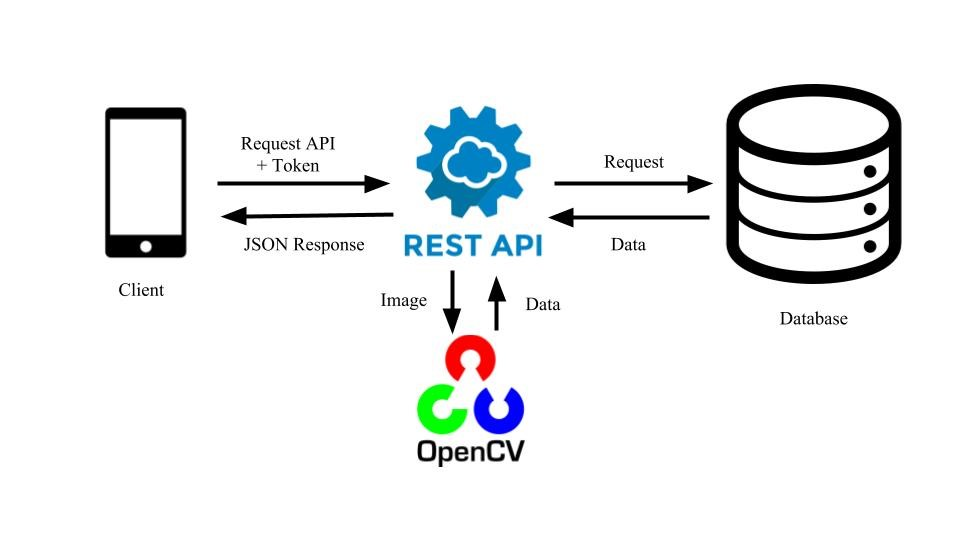
\includegraphics[width=\columnwidth]{Figures/3/project-structure}
		\caption{ภาพรวมของแอปพลิเคชันค้นหายาเพื่อคุณ}
		\label{Fig:project-structure}
	\end{figure}
	\subsection{ส่วนแอปพลิเคชัน}

		ส่วนแอปพลิเคชันผู้ใช้งานสามารถใช้งานฟังก์ชันดังต่อไปนี้

	\begin{enumerate}
		\item สามารถค้นหายาเม็ดแบบทั่วไป
		เป็นการค้นหาที่ใช้ key word ในการค้นหา เช่น para, น้ำเงิน, ส้ม, CAPSULE เป็นต้น 
		\item สามารถค้นหายาเม็ดแบบขั้นสูง
		เป็นการค้นหาที่ต้องใช้การระบุเอกลักษณ์ของยาเม็ดหรือแคปซูลแบบเจาะจง ลักษณะทางกายภาพหรือข้อมูลรายละเอียดต่างๆ
		\item สามารถดูรายละเอียดยาเม็ด
		เป็นการดูรายละเอียดของยาเม็ดหรือแคปซูลนั้นๆ ได้ทั้งดูรูปภาพ ข้อมูลยาต่างๆ เช่น ผู้ผลิต ผู้รับอนุญาติ ผู้จำหน่วย ขนาด กว้าง ยาว รูปแบบผลิตภัณฑ์ รูปร่าง ประเภทของยา เป็นต้น
		\item สามารถดูรายการยา
		เป็นการแสดงรายการยาที่เป็นผลลัพธ์จากการค้นหายาเม็ดแบบทั่ว การค้นหายาแบบขั้งสูง และรายการบุ๊กมาร์กยา
		\item สามารถกดบันทึกบุ๊กมาร์กรายการยา
		เพื่อบันทึกลงบนเครื่องผู้ใช้งานและดูย้อนหลังได้
		\item สามารถดูรายการบุ๊กมาร์กยา
		เป็นการดูรายการบุ๊กมาร์กยาที่ผู้ใช้งานกดบันทึกบุ๊กมาร์ก
		\item ถ่ายรูปภาพยาเม็ดเพื่อพิสูจน์เอกลักษณ์ยา
		เป็นการเปิดกล้องเพื่อถ่ายรูปภาพยาเม็ดและส่งรูปภาพไปประมวลผลที่ API service 
	\end{enumerate}

	\subsection{ส่วนเว็บเซอร์วิส}
	เว็บเซอร์วิสใช้เป็นสื่อในการแลกเปลี่ยนข้อมูลกันระหว่างแอปพลิเคชันและฐานข้อมูลในรูปแบบ JSON 
	โดยจะเรียกว่า API (Application Programming Interface) 
	ที่จะคอยกระทำการต่างๆ เช่น การดึงข้อมูลยา การประมวลผลรูปภาพ เป็นต้น 
	และส่วนเว็บเซอร์วิสมีหน้าที่การทำงานดังต่อไปนี้
	\begin{enumerate}
		\item สามารถติดต่อกับฐานข้อมูลการพิสูจน์เอกลักษณ์ยาเม็ดหรือแคปซูลของหน่วยข้อมูลยาและสุขภาพ คณะเภสัชศาสตร์ มหาวิทยาลัยอุบลราชธานี 
		\item สามารถค้นหาเม็ดยากับฐานข้อมูลการพิสูจน์เอกลักษณ์ยาเม็ดหรือแคปซูล 
		โดยการใช้พารามิเตอร์จากการร้องขอทรัพยากร (Request) ของแอปพลิเคชัน เช่น สี รูปทรง ขนาด ชื่อการค้า ชื่อสามัญ เป็นต้น 
		\item สามารถพิสูจน์ตัวตนของผู้ใช้งาน 
		เว็บเซอร์วิสมีการพิสูจน์ตัวตนผู้ใช้งานก่อนเรียกใช้งานการร้องขอด้วย JSON Web Token 
		เพื่อป้องกันการเรียกใช้งานจากผู้ที่ไม่พึ่งประสงค์ 
		\item สามารถถอดรหัสรูปภาพแบบ base64 
		\item สามารถประมวลผลภาพเพื่อหาลักษณะของเม็ดยา 
		ได้แก่ รูปทรง ขนาดและสี 
	\end{enumerate}

\newpage
\section{Use Case Diagram}
	Use Case Diagram เป็นแผนผังเพื่อแสดงฟังก์ชันแสดงการทำงานของระบบโดยรวม แสดงส่วนประกอบในระบบและกิจกรรมที่เกิดขึ้นในระบบ สัญลักษณ์ที่ใช้ในการเขียน Use Case Diagram แสดงในตารางที่ \ref{tab:use-case}

	\begin{table}[H]
		\centering
		\caption{สัญลักษณ์ของ Use case Diagram}
		\label{tab:use-case}
		\begin{tabular}{|c|p{10cm}|}
		\hline
		\textbf{สัญลักษณ์} & \multicolumn{1}{c|}{\textbf{การใช้งาน}} \\ \hline
		\raisebox{-\totalheight}{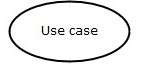
\includegraphics[width=0.3\textwidth]{Figures/table/use-case/1}}
		& \setstretch{1.5} {Use case คือส่วนย่อยของระบบงาน แทนด้วยวงรีและชื่อของ Use case ภายในวงรี} \\ \hline
		\raisebox{-\totalheight}{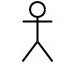
\includegraphics[height=1.5cm]{Figures/table/use-case/2}}
		& \setstretch{1.5} {Actor คือบุคคลหรือระบบงานอื่นที่ใช้งานระบบหรือได้รับประโยชน์จากระบบซึ่งอยู่ภายนอกระบบ แทนด้วยรูปคนและมีชื่อบทบาทการใช้งานระบบ} \\ \hline
		\raisebox{-\totalheight}{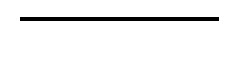
\includegraphics[width=3cm]{Figures/table/use-case/3}}
		& \setstretch{1.5} {เส้นตรงที่แสดงถึงการใช้งาน Use case ของผู้กระทำ} \\ \hline
		\raisebox{-\totalheight}{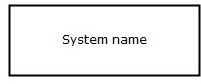
\includegraphics[width=0.3\textwidth]{Figures/table/use-case/4}}
		& \setstretch{1.5} {กรอบสี่เหลี่ยมแสดงถึงขอบเขตของระบบโดยแสดงชื่อระบบภายในหรือด้านบนกรอกสี่เหลี่ยม Use case อยู่ภายในกรอบสี่เหลี่ยม และ actor อยู่ภายนอกกรอบสี่เหลี่ยม} \\ \hline
		\raisebox{-\totalheight}{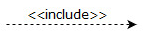
\includegraphics[width=0.3\textwidth]{Figures/table/use-case/5}}
		& \setstretch{1.5} {ความสัมพันธ์แบบ <<includes>> แสดงว่า Use case หนึ่งดำเนินการตามขั้นตอนของ Use case อื่น โดยแทนด้วยสัณลักษณ์ลูกศรเส้นประ ซึ่ง Use case ที่หางลูกศรเรียกใช้งาน Use case ที่หัวลูกศรทุกครั้งที่มีการทำงาน} \\ \hline
		\raisebox{-\totalheight}{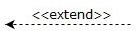
\includegraphics[width=0.3\textwidth]{Figures/table/use-case/6}}
		& \setstretch{1.5} {ความสัมพันธ์แบบ <<extend>> แสดงว่า Use case หนึ่งดำเนินการตามขั้นตอนของ Use case อื่น โดยแทนด้วยสัญลักษณ์ลูกศรเส้นประ ซึ่ง Use case ที่หัวลูกศรเรียกใช้งาน Use case ที่หางลูกศร แต่การใช้งานไม่จำเป็นต้องเกิดขึ้นทุกครั้งขึ้นอยู่กับเงื่อนไขระหว่างการทำงาน} \\ \hline
		\end{tabular}
	\end{table}

	\begin{figure}[H]
		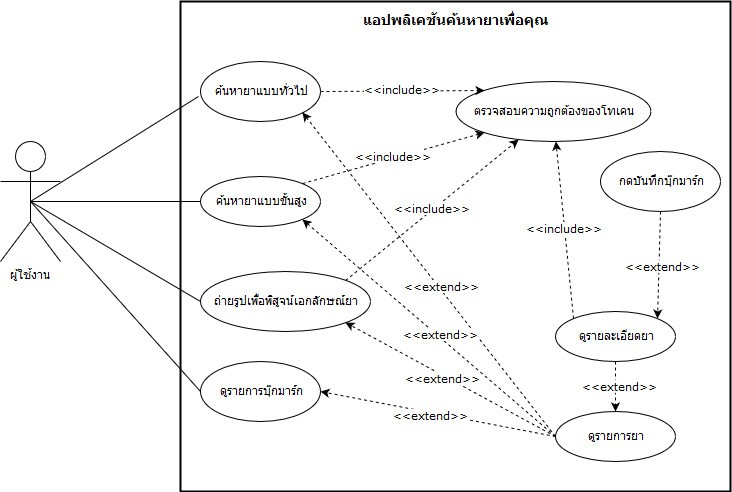
\includegraphics[width=\columnwidth]{Figures/3/case-use}
		\caption{Use Case Diagram ของแอปพลิเคชันค้นหายาเพื่อคุณ}
		\label{Fig:case-use}
	\end{figure}
	ในการพัฒนาแอปพลิเคชันค้นหายาเพื่อคุณสามารถอธิบายขั้นตอนการทำงานที่สำคัญและความสัมพันธ์ต่างๆ ของระบบด้วย Use Case Diagram แสดงดังรูปที่ \ref{Fig:case-use} ซึ่งประกอบด้วย Use case ต่างๆ ดังนี้

	\begin{enumerate}
		\item ค้นหายาแบบทั่วไป : ทำหน้าที่การสืบค้นแบบให้ผู้ใช้งานกรอกคำสำคัญ เช่น ชื่อบริษัท ชื่อการค้า รูปร่าง สี ขนาด เป็นต้น
		\item ค้นหายาแบบขั้นสูง : ทำหน้าที่การสืบค้นแบบให้ผู้ใช้งานกรอกรายละเอียดของยาเม็ด เช่น รูปร่าง สี ขนาด เป็นต้น
		\item ถ่ายรูปเพื่อพิสูจน์เอกลักษณ์ยา : ทำหน้าที่ให้ผู้ใช้งานถ่ายรูปภาพยาเม็ดเพื่อการพิสูจน์เอกลักษณ์ยาเม็ด
		\item ดูรายการยา : ทำหน้าที่แสดงรายการยาจากการค้นหายาแบบทั่วไป ค้นหายาแบบขั้นสูง การถ่ายรูปเพื่อพิสูจน์เอกลักษณ์ยา และการดูรายการบุ๊กมาร์ก
		\item ดูรายละเอียดยา : ทำหน้าที่แสดงรายละเอียดของยาเม็ดให้แก่ผู้ใช้งาน
		\item กดบันทึกบุ๊กมาร์กยา : ทำหน้าที่บันทึกรายการยาเอาไว้ในเครื่องผู้ใช้งาน
		\item ดูรายการบุ๊กมาร์ก : ทำหน้าที่แสดงรายการบุ๊กมาร์กทั้งหมดที่ผู้ใช้กดบันทึกในเครื่องผู้ใช้งาน
		\item ตรวจสอบความถูกต้องของโทเคน : ทำหน้าที่ตรวจสอบความถูกต้องของโทเคนของแอปพลิเคชันกับเว็บเซอร์วิส ก่อนจะสามารถใช้งานแอปพลิเคชั่นได้
	\end{enumerate}

\newpage
\section{Class Diagram}
	Class Diagram คือแผนภาพที่ใช้แสดงคลาสและความสัมพันธ์ในแบบต่างๆ ระหว่างคลาส สัญลักษณ์ที่ใช้ในการเขียน Class Diagram แสดงในตารางที่ \ref{tab:class} 
	\begin{center}
	\begin{table}[H]
		\centering
		\caption{สัญลักษณ์ของ Class Diagram}
		\label{tab:class}
		\begin{tabular}{|c|p{10cm}|}
		\hline
		\textbf{สัญลักษณ์} & \multicolumn{1}{c|}{\textbf{การใช้งาน}} \\ \hline
		\raisebox{-\totalheight}{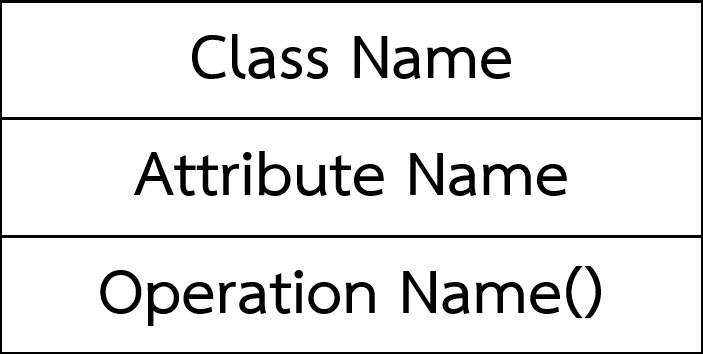
\includegraphics[width=0.3\textwidth]{Figures/table/class/11}}
		& \setstretch{1.5} {Class สัญลักษณ์แทนด้วยสี่เหลี่ยมแบ่งเป็น 3 ส่วน ส่วนบนเป็นชื่อ Class ส่วนกลางเป็น Attribute และส่วนล่างเป็น Operation Name หรือ Method ซึ่งคลาสเป็นสิ่งที่เก็บรวบรวมข้อมูลที่แสดงถึงบุคคล สถานที่ เหตุการณ์หรือสิ่งต่างๆ ที่มีความเกี่ยวข้องกับระบบ Method เป็นการกระทำหรือฟังก์ชันที่คลาสนั้นสามารถทำได้} \\ \hline
		Method Name()
		& \setstretch{1.5} {Method สามารถแบ่งการมองเห็น (Visibility) ได้ 3 ชนิดได้แก่ 
			\begin{enumerate}
				\item Public แทนสัญลักษณ์ด้วยเครื่องหมายบวก (+)
				\item Private แทนสัญลักษณ์ด้วยเครื่องหมายบวก (-)
				\item Protected แทนสัญลักษณ์ด้วยเครื่องหมายบวก (\#)
			\end{enumerate}
		} \\ \hline
		\raisebox{-\totalheight}{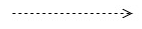
\includegraphics[width=0.3\textwidth]{Figures/table/class/1}}
		& \setstretch{1.5} {Dependency Relationship หมายความว่า คลาสที่อยู่ฝั่งต้นลูกศรสามารถเรียกใช้คลาสที่อยู่ฝั่งหัวลูกศร} \\ \hline
		\raisebox{-\totalheight}{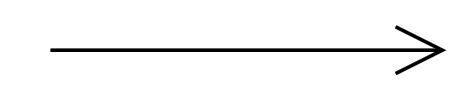
\includegraphics[width=0.3\textwidth]{Figures/table/class/4}}
		& \setstretch{1.5} Generalization หมายความว่า คลาสที่อยู่ฝั่งต้นลูกศรทำการสืบทอดคลาสที่อยู่หัวลูกศร} \\ \hline
		\raisebox{-\totalheight}{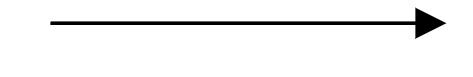
\includegraphics[width=0.3\textwidth]{Figures/table/class/5}}
		& \setstretch{1.5} {Association Relationship หมายความว่า คลาสที่อยู่ฝั่งต้นลุกศรทำการกำหนดคลาสอื่นในรูป Attribute ภายในคลาส และสามารถเรียกใช้ Method จากคลาสนั้นได้} \\ \hline
		\end{tabular}
	\end{table}
	\end{center}
	% \begin{table}[H]
	% 	\caption{สัญลักษณ์ของ Class Diagram}
	% 	\label{tab:class}		
	% 	\begin{tabular}{c}
	% 		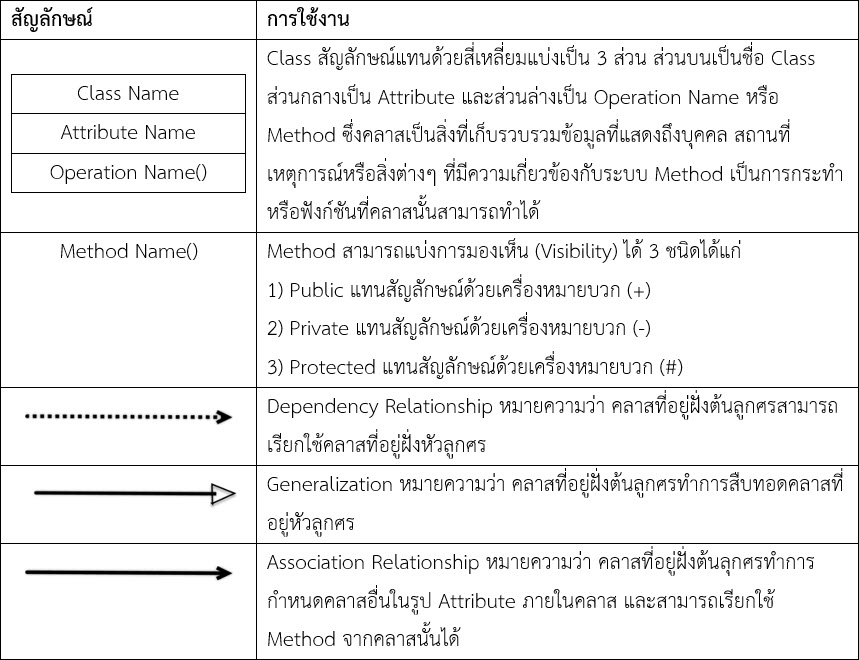
\includegraphics[width=\columnwidth]{Figures/table/class}	\\ 
	% 	\end{tabular}
	% \end{table}

	Class Diagram แสดงความสัมพันธ์ในรูปแบบต่างๆ ระหว่างคลาสของแอปพลิเคชันค้นหายาเพื่อคุณ อธิบายได้ตามรูปที่ \ref{Fig:class} ดังต่อไปนี้

	\begin{figure}[H]
		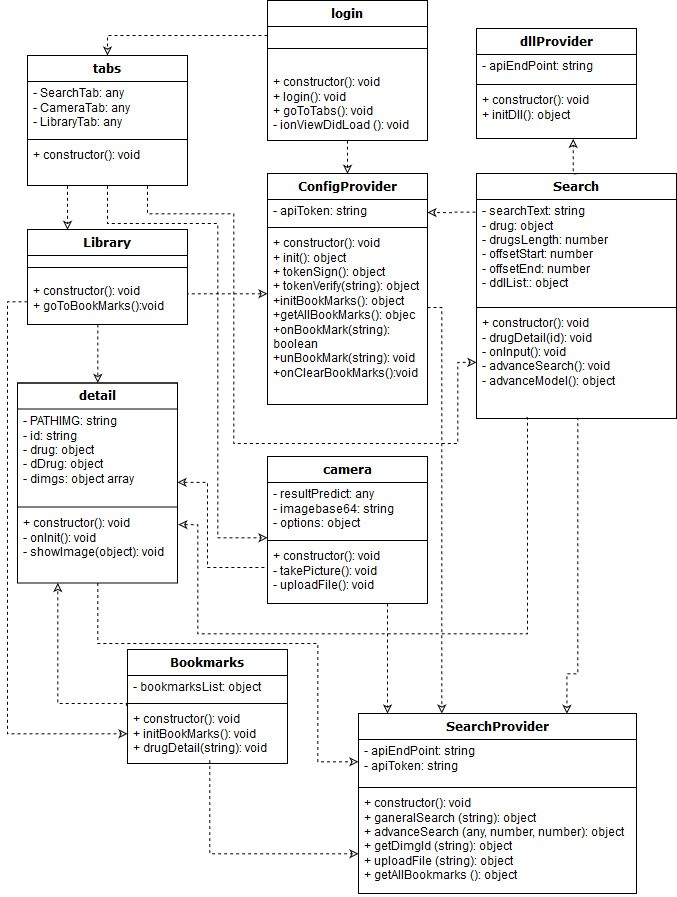
\includegraphics[width=\columnwidth]{Figures/3/class}
		\caption{Class Diagram ของแอปพลิเคชันค้นหายาเพื่อคุณ}
		\label{Fig:class}
	\end{figure}

	\newpage
	จากรูปที่ \ref{Fig:class} สามารถอธิบายแผนภาพ Class Diagram ได้ดังต่อไปนี้
	\begin{enumerate}
		\item Class Login เป็นคลาสที่แสดงหน้าแรกของแอปพลิเคชัน เพื่อเข้าสู่ระบบอัตโนมัติโดยจะทำงานร่วมกันคลาส ConfigProvider สำหรับการตรวจสอบความถูกต้องของโทเคนหรือการร้องขอโทเคนจากเว็บเซอร์วิสในการใช้แอปพลิเคชัน 
		\item Class Tabs เป็นคลาสที่จัดการและแสดงหน้าแท็บทั้ง 2 คลาส ได้แก่ คลาส Search และคลาส Camera 
		\item Class ConfigProvider เป็นคลาสที่กำหนดค่าเริ่มต้นของแอปพลิเคชัน ได้แก่ การร้องขอโทเคนจากเว็บเซอร์วิส และการตรวจสอบความถูกต้องของโทเคน 
		\item Class Camera เป็นคลาสที่เปิดการทำงานของกล้องถ่ายรูปเพื่อให้ถ่ายรูปและประมวลผลภาพ
		\item Class Search เป็นคลาสที่แสดงหน้าการค้นหายาแบบทั่วไปและการค้นหายาแบบละเอียด โดยจะทำงานร่วมกับคลาส SearchProvider สำหรับใช้ร้องขอไปที่เว็บเซอร์วิสเพื่อค้นหายา และทำงานร่วมกับคลาส dllProvider สำหรับใช้ร้องขอไปที่เว็บเซอร์วิสเพื่อดึงรายการ dropdown มาแสดง
		\item Class Library เป็นคลาสที่แสดงรายการคำสั่งในการจัดการกับรายการบุ๊กมาร์กยา 
		\item Class Bookmarks เป็นคลาสที่แสดงรายการบุ๊กมาร์กของผู้ใช้งานที่ถูกเก็บไว้ในเครื่องผู้ใช้งาน 
		\item Class SearchProvider เป็นคลาสที่จัดการการเชื่อมต่อกับเว็บเซอร์วิส ได้แก่ การร้องขอไปยังเว็บเซอร์วิสเพื่อการค้นหาทั่วไปกับการค้นหาแบบละเอียด การร้องขอไปยังเว็บเซอร์วิสเพื่อการดึงข้อมูลยาแบบละเอียด
		\item Class Detail เป็นคลาสที่แสดงข้อมูลยาแบบละเอียดที่ได้มาจากคลาส SearchProvider 
		\item Class dllProvider เป็นคลาสที่จัดการกับรายการ dropdown ที่ร้องข้อไปยังเว็บเซอร์วิส 
	\end{enumerate}

\newpage
\section{Sequence Diagram}
	Sequence Diagram เป็น Diagram ที่แสดงขั้นตอนการทำงานของแต่ละ Use Case ระหว่าง Object ต่างๆ ที่ส่งข้อความถึงกันและกัน โดย Sequence Diagram จะช่วยให้มองเห็นการทำงานของภาพรวมของระบบ ส่วนประกอบสัญลักษณ์ที่ใช้ในการเขียน Sequence Diagram 
	แสดงดังตารางที่ \ref{tab:Sequences}
	
	\begin{table}[H]
		\centering
		\caption{สัญลักษณ์ของ Sequence Diagram}
		\label{tab:Sequences}
		\begin{tabular}{| c	| p{10cm} |}
		\hline
		\textbf{สัญลักษณ์} & \multicolumn{1}{c|}{\textbf{การใช้งาน}} \\ \hline
		\raisebox{-\totalheight}{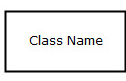
\includegraphics[width=0.2\textwidth]{Figures/table/Sequence/Sequence1}}
		& \setstretch{1.5} {Class แสดงถึงการทำงานของ Use Case ในการส่งหรือรับข้อความ แทนด้วยสัญลักษณ์สี่เหลี่ยมมีชื่อคลาสอยู่ภายใน} \\ \hline
		\raisebox{-\totalheight}{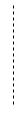
\includegraphics[height=0.1\textheight]{Figures/table/Sequence/Sequence2}}
		& \setstretch{1.5} {Lifeline หรือเส้นอายุขัย แสดงช่วงเวลาตั้งแต่เริ่มสร้าง object ในคลาสนั้น จนกระทั่ง object นั้นถูกทำลาย สัญลักษณ์แทนด้วยเส้นประ} \\ \hline
		\raisebox{-\totalheight}{
\includegraphics[height=0.1\textheight]{Figures/table/Sequence/Sequence3}}
		& \setstretch{1.5} {Focus of control หรือจุดควบคุม เป็นจุดควบคุมที่ object ใช้ทำการส่งหรือรับข้อความ สัญลักษณ์แทนด้วยสี่เหลี่ยม} \\ \hline
		\raisebox{-\totalheight}{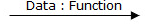
\includegraphics[width=0.3\textwidth]{Figures/table/Sequence/Sequence4}}
		& \setstretch{1.5} {Message คือ ข้อความที่รับส่งระหว่าง Object สัญลักษณ์แทนด้วยลูกศรและประกอบด้วย 2 ส่วน คือ ข้อมูล (Data) และฟังก์ชัน (Function)} \\ \hline
		\raisebox{-\totalheight}{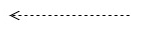
\includegraphics[width=0.3\textwidth]{Figures/table/Sequence/Sequence5}}
		& \setstretch{1.5} {Return Message เป็นข้อมูลที่ส่งกลับหลังจากทำงานเสร็จ} \\ \hline
		\end{tabular}
	\end{table}

	Sequence Diagram ที่ใช้อธิบายการทำงานของแอปพลิเคชันค้นหายาเพื่อคุณซึ่งประกอบไปด้วย 
	การค้นหายาแบบทั่วไป การค้นหายาแบบขั้งสูง การถ่ายรูปเพื่อพิสูจน์เอกลักษณ์ยา และการดูรายละเอียดยา 
	โดยมีรายละเอียดดังต่อไปนี้
	\subsection{Sequence Diagram ของการค้นหายาแบบทั่วไป}

	\begin{figure}[H]
		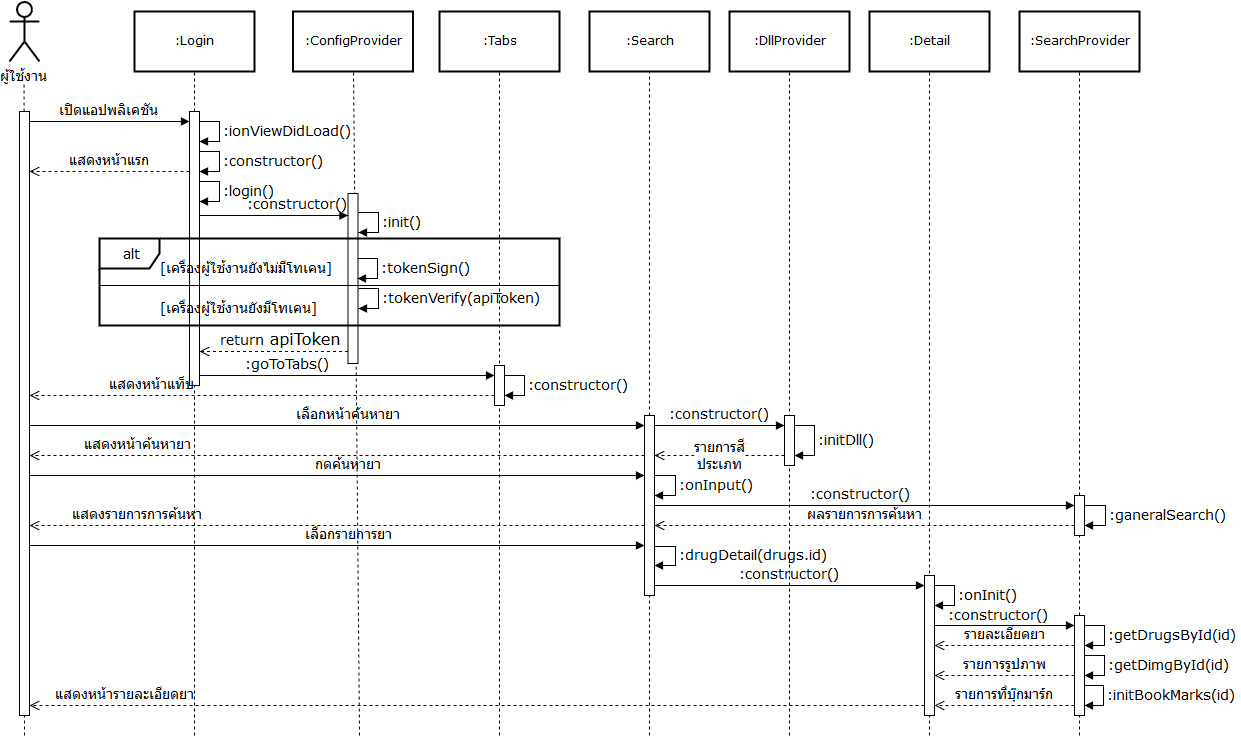
\includegraphics[width=\columnwidth]
		{Figures/3/Sequence-1}
		\caption{Sequence Diagram ของการค้นหายาแบบทั่วไป}
		\label{Fig:Sequence-1}
	\end{figure}

	จากรูปที่ \ref{Fig:Sequence-1} Sequence Diagram ของการค้นหายาแบบทั่วไป 
	สามารถอธิบายได้ดังนี้ 
	เมื่อผู้ใช้งานเปิดแอปพลิเคชันค้นหายาเพื่อคุณ 
	ระบบจะเริ่มต้นการทำที่คลาส Login ด้วยฟังก์ชัน ionViewDidLoad และ constructor 
	เพื่อสร้างหน้าแรกและแสดงหน้าแรกให้ผู้ใช้งาน 
	หลังจากนั้นระบบจะเรียกใช้งานฟังก์ชัน Login 
	และในขณะเดียวกันก็จะเรียกใช้งานคลาส ConfigProvider ฟังก์ชัน Constructor 
	เพื่อเรียกใช้งานฟังก์ชัน init สำหรับกำหนดค่าเริ่มต้นของโทเคน 
	โดยจะมีเงื่อนไขในตรวจสอบเครื่องผู้ใช้งานมีโทเคนหรือไม่ 
	ถ้าหากไม่มีโทเคนจะเรียกใช้งานฟังก์ชัน tokenSign 
	และถ้าหากมีโทเคนจะเรียกใช้งานฟังก์ชัน tokenVerify 
	หลังจากนั้นจะคืน apiToken ที่เป็นผลลัพธ์กลับมาที่คลาส Login 
	และดำเนินการต่อไปด้วยฟังก์ชัน goToTabs 
	สำหรับเรียกใช้งานคลาส Tabs ฟังก์ชัน constructor 
	เพื่อสร้างหน้าแท็บและแสดงหน้าแท็กให้ผู้ใช้งาน 
	จากนั้นเรียกใช้งานคลาส Search ฟังก์ชัน constructor 
	และเรียกใช้งาน DllProvider ฟังก์ชัน initDll 
	เพื่อสร้างหน้าค้นหาและแสดงหน้าค้นหาให้ผู้ใช้งาน 
	เมื่อผู้ใช้งานกดค้นหายาที่หน้าค้นาหายา จะเรียกใช้งานคลาส Search ฟังก์ชัน onInput 
	หลังจากนั้นจะเรียกใช้งานคลาส SearchProvider ฟังก์ชัน constructor 
	และฟังก์ชัน ganeralSearch เพื่อร้องขอการค้นหาไปที่เว็บเซอร์วิสและส่งข้อมูลรายการการค้าหายากลับมายังคลาส Search 
	จากนั้นแสดงที่หน้ารายการค้าหาให้ผู้ใช้งาน 
	เมื่อผู้ใช้งานเลือกรายการยา จะเรียกใช้งานคลาส Search ฟังก์ชัน drugDetail 
	พร้อมกับส่งหมายเลขยาไปกับฟังก์ชัน drugDetail ไปที่คลาส Detail ฟังก์ชัน constructor 
	และฟังก์ชัน onInit เพื่อร้องขอข้อมูลยาจากเว็บเซอร์วิสที่คลาส SearchProvider ผ่านทางฟังก์ชัน getDrugById เพื่อร้องขอข้อมูลรายละเอียดยา และผ่านทางฟังก์ชัน getDimgById 
	เพื่อร้องขอข้อมูลรูปภาพ และฟังก์ชัน initBookMarks เพื่อตรวจสอบรายการที่ถูกบุ๊กมาร์กไว้ 
	และแสดงหน้ารายละเอียดยาแก่ผู้ใช้งาน
	
	\subsection{Sequence Diagram ของการค้นหายาแบบขั้นสูง}

	\begin{figure}[H]
		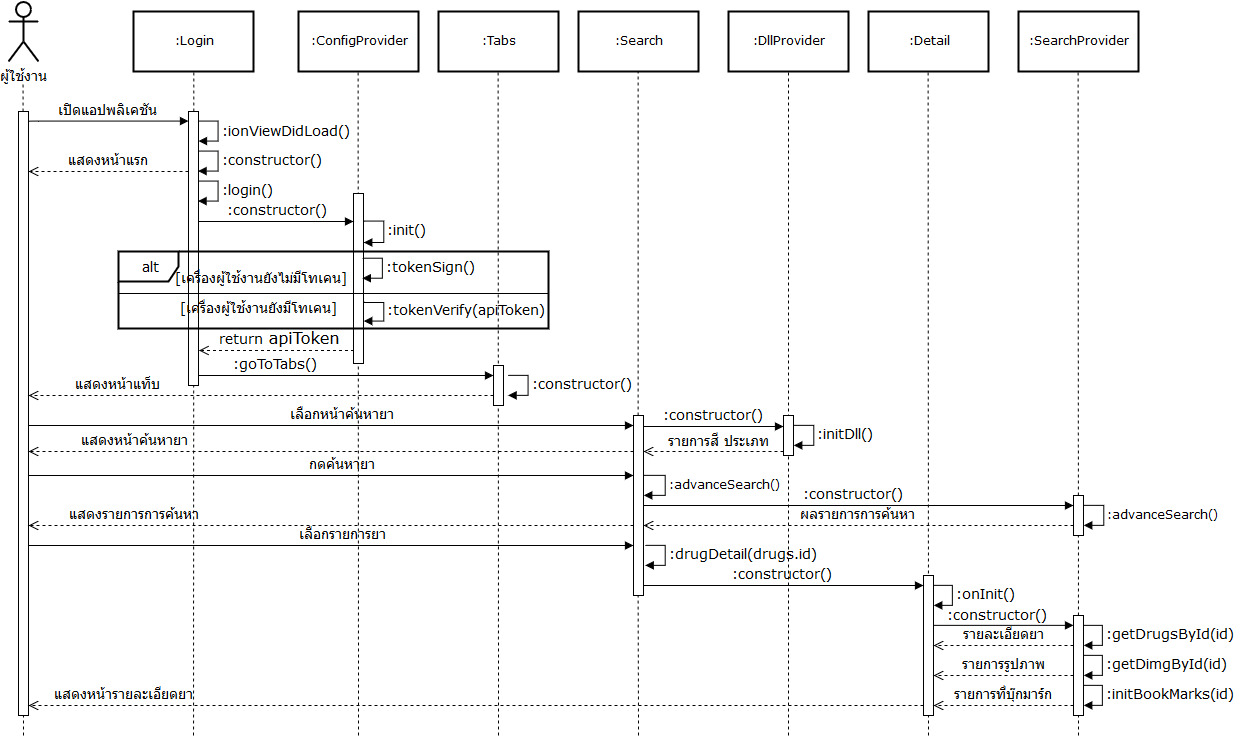
\includegraphics[width=\columnwidth]
		{Figures/3/Sequence-2}
		\caption{Sequence Diagram ของการค้นหายาแบบขั้นสูง}
		\label{Fig:Sequence-2}
	\end{figure}
	
	จากรูปที่ \ref{Fig:Sequence-2} Sequence Diagram ของการค้นหายาแบบขั้นสูง สามารถอธิบายได้ดังนี้ เมื่อผู้ใช้งานเปิดแอปพลิเคชันค้นหายาเพื่อคุณ ระบบจะเริ่มต้นการทำที่คลาส Login ด้วยฟังก์ชัน ionViewDidLoad และ constructor เพื่อสร้างหน้าแรกและแสดงหน้าแรกให้ผู้ใช้งาน หลังจากนั้นระบบจะเรียกใช้งานฟังก์ชัน Login และในขณะเดียวกันก็จะเรียกใช้งานคลาส ConfigProvider ฟังก์ชัน Constructor เพื่อเรียกใช้งานฟังก์ชัน init สำหรับกำหนดค่าเริ่มต้นของโทเคน โดยจะมีเงื่อนไขในตรวจสอบเครื่องผู้ใช้งานมีโทเคนหรือไม่ ถ้าหากไม่มีโทเคนจะเรียกใช้งานฟังก์ชัน tokenSign และถ้าหากมีโทเคนจะเรียกใช้งานฟังก์ชัน tokenVerify หลังจากนั้นจะคืน apiToken ที่เป็นผลลัพธ์กลับมาที่คลาส Login และดำเนินการต่อไปด้วยฟังก์ชัน goToTabs สำหรับเรียกใช้งานคลาส Tabs ฟังก์ชัน constructor เพื่อสร้างหน้าแท็บและแสดงหน้าแท็กให้ผู้ใช้งาน จากนั้นเรียกใช้งานคลาส Search ฟังก์ชัน constructor และเรียกใช้งาน DllProvider ฟังก์ชัน initDll เพื่อสร้างหน้าค้นหาและแสดงหน้าค้นหาให้ผู้งาน เมื่อผู้ใช้งานกดค้นหายา คลาส Search ฟังก์ชัน advanceSearch ในขณะเดียวกันจะเรียกใช้งานคลาส SearchProvider ฟังก์ชัน constructor และฟังก์ชัน advanceSearch เพื่อร้องขอการค้นหาไปที่เว็บเซอร์วิสและส่งข้อมูลรายการการค้าหายากลับมายังคลาส Search จากนั้นแสดงที่หน้ารายการค้าหาให้ผู้ใช้งาน เมื่อผู้ใช้งานเลือกรายการยา จะเรียกใช้งานคลาส Search ฟังก์ชัน drugDetail พร้อมกับส่งหมายเลขยาไปกับฟังก์ชัน ไปที่คลาส Detail ฟังก์ชัน constructor และฟังก์ชัน onInit เพื่อร้องขอข้อมูลยาจากเว็บเซอร์วิสที่คลาส SearchProvider ผ่านทางฟังก์ชัน getDrugById เพื่อร้องขอข้อมูลรายละเอียดยา และผ่านทางฟังก์ชัน getDimgById เพื่อร้องขอข้อมูลรูปภาพ และฟังก์ชัน initBookMarks เพื่อตรวจสอบรายการที่ถูกบุ๊กมาร์กไว้ และแสดงหน้ารายละเอียดยาแก่ผู้ใช้งาน

	\subsection{Sequence Diagram ของการถ่ายรูปภาพเพื่อพิสูจน์เอกลักษณ์ยาเม็ด}	

	\begin{figure}[H]
		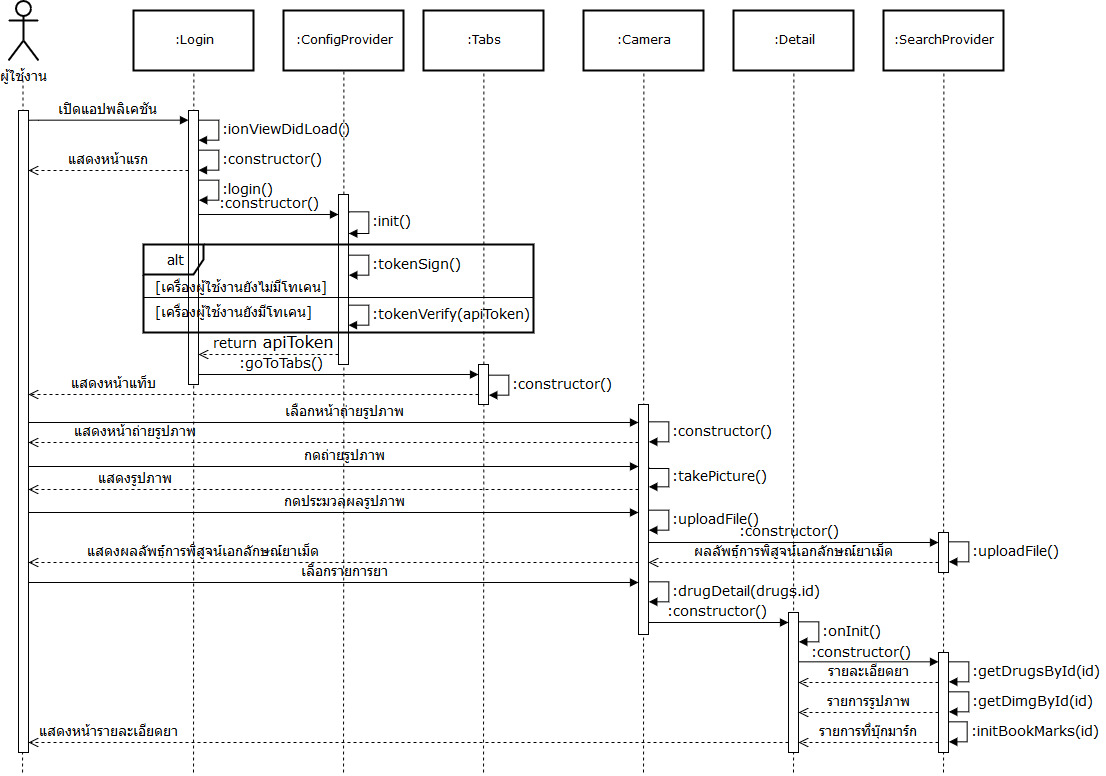
\includegraphics[width=\columnwidth]{Figures/3/Sequence-3}
		\caption{Sequence Diagram ของการถ่ายรูปภาพเพื่อพิสูจน์เอกลักษณ์ยาเม็ด}
		\label{Fig:Sequence-3}
	\end{figure}

	จากรูปที่ \ref{Fig:Sequence-3} Sequence Diagram ของการถ่ายรูปภาพเพื่อพิสูจน์เอกลักษณ์ยาเม็ด สามารถอธิบายได้ดังนี้ เมื่อผู้ใช้งานเปิดแอปพลิเคชันค้นหายาเพื่อคุณ ระบบจะเริ่มต้นการทำที่คลาส Login ด้วยฟังก์ชัน ionViewDidLoad และ constructor เพื่อสร้างหน้าแรกและแสดงหน้าแรกให้ผู้ใช้งาน หลังจากนั้นระบบจะเรียกใช้งานฟังก์ชัน Login และในขณะเดียวกันก็จะเรียกใช้งานคลาส ConfigProvider ฟังก์ชัน Constructor เพื่อเรียกใช้งานฟังก์ชัน init สำหรับกำหนดค่าเริ่มต้นของโทเคน โดยจะมีเงื่อนไขในตรวจสอบเครื่องผู้ใช้งานมีโทเคนหรือไม่ ถ้าหากไม่มีโทเคนจะเรียกใช้งานฟังก์ชัน tokenSign และถ้าหากมีโทเคนจะเรียกใช้งานฟังก์ชัน tokenVerify หลังจากนั้นจะคืน apiToken ที่เป็นผลลัพธ์กลับมาที่คลาส Login และดำเนินการต่อไปด้วยฟังก์ชัน goToTabs สำหรับเรียกใช้งานคลาส Tabs ฟังก์ชัน constructor เพื่อสร้างหน้าแท็บและแสดงหน้าแท็กให้ผู้ใช้งาน จากนั้นเรียกใช้งานคลาส Camera ฟังก์ชัน constructor เพื่อสร้างหน้าการถ่ายรูปเพื่อพิสูจน์เอกลักษณ์ยา เมื่อผู้ใช้งานกดถ่ายรูปภาพยาจะเรียกใช้งานฟังก์ชัน takePicture และจะแสดงรูปรูปที่ถ่ายได้ให้ผู้ใช้งาน เมื่อผู้ใช้งานกดประมวลผลภาพจะเรียกใช้งานฟังก์ชัน uploadFile ในขณะเดียวกันจะเรียกใช้งานคลาส SearchProvider ฟังก์ชัน constructor และฟังก์ชัน uploadFile เพื่อร้องขอไปประมวลผลภาพที่เว็บเซอร์วิสและส่งผลลัพธ์กลับมาที่คลาส Camera เพื่อแสดงผลลัพธ์การพิสูจน์เอกลักษณ์ยาให้ผู้ใช้งาน เมื่อผู้ใช้งานเลือกรายการยา จะเรียกใช้งานคลาส Search ฟังก์ชัน drugDetail พร้อมกับส่งหมายเลขยาไปกับฟังก์ชัน ไปที่คลาส Detail ฟังก์ชัน constructor และฟังก์ชัน onInit เพื่อร้องขอข้อมูลยาจากเว็บเซอร์วิสที่คลาส SearchProvider ผ่านทางฟังก์ชัน getDrugById เพื่อร้องขอข้อมูลรายละเอียดยา และผ่านทางฟังก์ชัน getDimgById เพื่อร้องขอข้อมูลรูปภาพ และฟังก์ชัน initBookMarks เพื่อตรวจสอบรายการที่ถูกบุ๊กมาร์กไว้ และแสดงหน้ารายละเอียดยาแก่ผู้ใช้งาน
	
	\subsection{Sequence Diagram ของการดูรายการบุ๊กมาร์ก}

	\begin{figure}[H]
		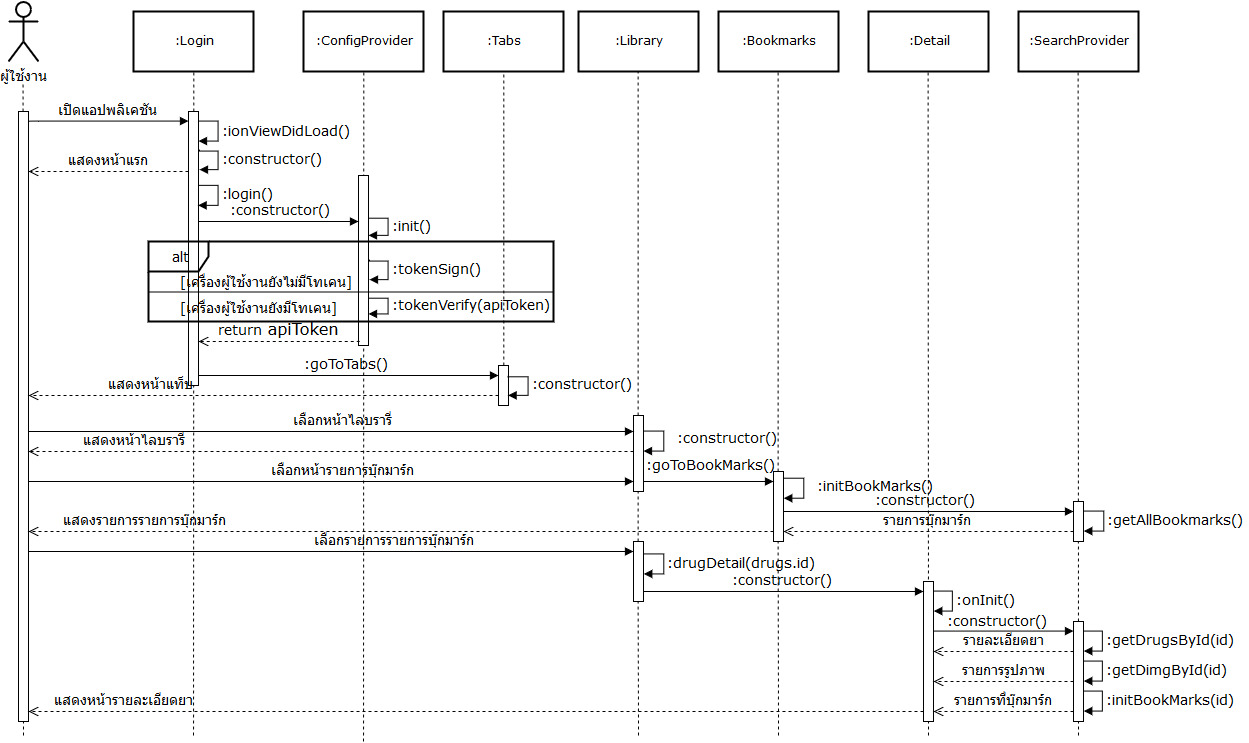
\includegraphics[width=\columnwidth]
		{Figures/3/Sequence-4}
		\caption{Sequence Diagram ของการดูรายการบุ๊กมาร์ก}
		\label{Fig:Sequence-4}
	\end{figure}

	จากรูปที่ \ref{Fig:Sequence-4} Sequence Diagram ของการดูรายละเอียดยา สามารถอธิบายได้ดังนี้ เมื่อผู้ใช้งานเปิดแอปพลิเคชันค้นหายาเพื่อคุณ ระบบจะเริ่มต้นการทำที่คลาส Login ด้วยฟังก์ชัน ionViewDidLoad และ constructor เพื่อสร้างหน้าแรกและแสดงหน้าแรกให้ผู้ใช้งาน หลังจากนั้นระบบจะเรียกใช้งานฟังก์ชัน Login และในขณะเดียวกันก็จะเรียกใช้งานคลาส ConfigProvider ฟังก์ชัน Constructor เพื่อเรียกใช้งานฟังก์ชัน init สำหรับกำหนดค่าเริ่มต้นของโทเคน โดยจะมีเงื่อนไขในตรวจสอบเครื่องผู้ใช้งานมีโทเคนหรือไม่ ถ้าหากไม่มีโทเคนจะเรียกใช้งานฟังก์ชัน tokenSign และถ้าหากมีโทเคนจะเรียกใช้งานฟังก์ชัน tokenVerify หลังจากนั้นจะคืน apiToken ที่เป็นผลลัพธ์กลับมาที่คลาส Login และดำเนินการต่อไปด้วยฟังก์ชัน goToTabs สำหรับเรียกใช้งานคลาส Tabs ฟังก์ชัน constructor เพื่อสร้างหน้าแท็บและแสดงหน้าแท็กให้ผู้ใช้งาน เมื่อผู้ใช้งานเลือกหน้าไลบรารี่ จะเรียกใช้งานคลาส Library ฟังก์ชัน goToBookMarks เพื่อเรียกใช้งานคลาส Bookmarks ฟังก์ชัน initBookMarks ในขณะเดียวกันจะเรียกใช้งานคลาส SearchProvider ฟังก์ชัน constructor และฟังก์ชัน getAllBookmarks เพื่อดึงรายการบุ๊กมาร์กจากเครื่องผู้ใช้งานมา จากนั้นจะแสดงหน้ารายการบุ๊กมาร์กให้ผู้ใช้งาน เมื่อผู้ใช้งานเลือกรายการยา จะเรียกใช้งานคลาส Search ฟังก์ชัน drugDetail พร้อมกับส่งหมายเลขยาไปกับฟังก์ชัน ไปที่คลาส Detail ฟังก์ชัน constructor และฟังก์ชัน onInit เพื่อร้องขอข้อมูลยาจากเว็บเซอร์วิสที่คลาส SearchProvider ผ่านทางฟังก์ชัน getDrugById เพื่อร้องขอข้อมูลรายละเอียดยา และผ่านทางฟังก์ชัน getDimgById เพื่อร้องขอข้อมูลรูปภาพ และฟังก์ชัน initBookMarks เพื่อตรวจสอบรายการที่ถูกบุ๊กมาร์กไว้ และแสดงหน้ารายละเอียดยาแก่ผู้ใช้งาน


\newpage
\section{State Diagram}
	State Diagram เป็นภาพแผนที่แสดงอ็อบเจ็กต์แต่ละตัว โดยสถานะรวมของระบบเกิดจากสถานะย่อยของอ็อบเจ็กต์แต่ละตัวรวมกันเป็นกลไกที่ทำให้ระบบมีการเปลี่ยนสถานะคือการส่ง message ในทาง Object orientation คือการเรียกใช้ฟังก์ชันของอ็อบเจ็กต์นั้นเอง ซึ่งส่วนประกอบและสัญลักษณ์ที่ใช้ในการเขียน State Diagram แสดงในตารางที่ \ref{tab:state}
	
	\begin{table}[H]
		\centering
		\caption{สัญลักษณ์ของ State Diagram}
		\label{tab:state}
		\begin{tabular}{| c	| p{10cm} |}
		\hline
		\textbf{สัญลักษณ์} & \multicolumn{1}{c|}{\textbf{การใช้งาน}} \\ \hline
		\raisebox{-\totalheight}{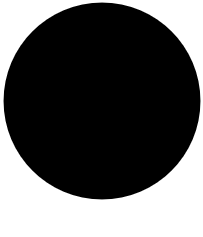
\includegraphics[width=8mm]{Figures/table/state/state1}}
		& \setstretch{1.5} {Initial state คือสถานะเริ่มต้นแสดงถึงอ็อบเจ็กต์ที่เกิดขึ้น} \\ \hline
		\raisebox{-\totalheight}{
\includegraphics[width=0.1\textwidth]{Figures/table/state/state2}}
		& \setstretch{1.5} {Initial state คือสถานะเริ่มต้นแสดงถึงอ็อบเจ็กต์ที่เกิดขึ้น} \\ \hline
		\raisebox{-\totalheight}{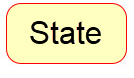
\includegraphics[width=0.2\textwidth]{Figures/table/state/state3}}
		& \setstretch{1.5} {State คือแสดงสถานะอ็อบเจ็กต์} \\ \hline
		\raisebox{-\totalheight}{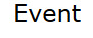
\includegraphics[width=0.2\textwidth]{Figures/table/state/state4}}
		& \setstretch{1.5} {Event คือเหตุการณ์ที่เกิดขึ้นทำให้เกิดการเปลี่ยนสถานะ โดยมีเงื่อนไข ซึ่งอ็อบเจ็กต์จะเปลี่ยนสถานะเมื่อเงื่อนไขดังกว่างเป็นจริง} \\ \hline
		\raisebox{-\totalheight}{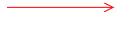
\includegraphics[width=0.3\textwidth]{Figures/table/state/state5}}
		& \setstretch{1.5} {Transition คือการเปลี่ยนสถานะแสดงถึงการเปลี่ยนสถานะของอ็อบเจ็กต์จากสถานะหนึ่งไปยังสถานะอื่น} \\ \hline
		\end{tabular}
	\end{table}


	State Diagram ใช้สำหรับอธิบายการทำงานของแอปพลิเคชันค้นหายาเพื่อคุณซึ่งประกอบไปด้วย ส่วนการค้นหายาและการแสดงรายละเอียดยา และส่วนการถ่ายรูปเพื่อการพิสูจน์เอกลักษณ์ยา โดยมีรายละเอียดดังต่อไปนี้

	\begin{figure}[H]
		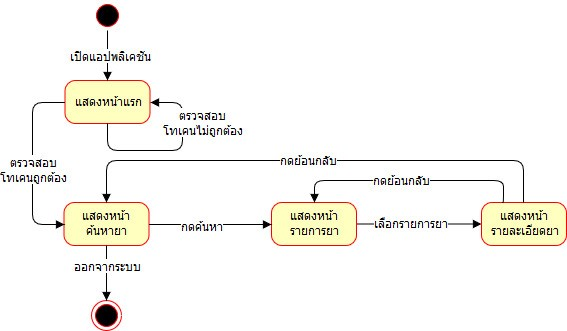
\includegraphics[width=\columnwidth]{Figures/3/state1}
		\caption{State Diagram ส่วนการค้นหายาและการแสดงรายละเอียดยา}
		\label{Fig:state1}
	\end{figure}

	จากรูปที่ \ref{Fig:state1} เป็น State Diagram ของส่วนการค้นหายาและการแสดงรายละเอียดยา สามารถอธิบายได้ดังต่อไปนี้ ผู้ใช้งานเปิดแอปพลิเคชันขึ้นมาระบบจะอยู่ในสถานะแสดงหน้าแรก เมื่อระบบตรวจสอบความถูกต้องของโทเคนสำเร็จ ระบบจะอยู่ในสถานะแสดงค้นหายา เมื่อผู้ใช้งานกดค้นหายาระบบจะอยู่ในสถานะแสดงหน้ารายการยา เมื่อผู้ใช้งานเลือกรายการยาเพื่อย้ายสถานะของระบบไปที่สถานะแสดงหน้ารายะเอียดยา จากนั้นผู้ใช้งานสามารถกดย้อนกลับ (รายการยา) เพื่อย้ายสถานะของระบบไปที่สถานะแสดงหน้ารายการยาและผู้ใช้งานสามารถกดย้อมกลับ (ค้นหายา) เพื่อย้ายสถานะของระบบไปที่สถานะแสดงหน้าค้นหา

	\begin{figure}[H]
		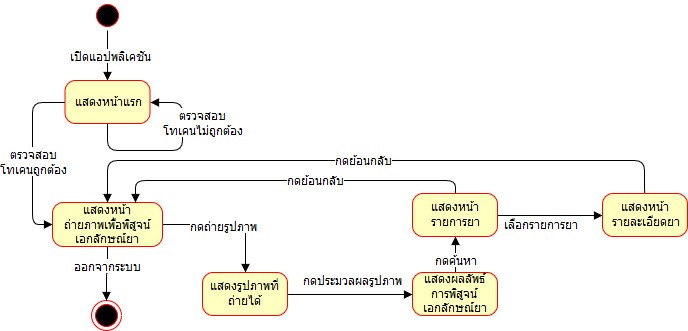
\includegraphics[width=\columnwidth]{Figures/3/state2}
		\caption{State Diagram ส่วนการถ่ายรูปเพื่อการพิสูจน์เอกลักษณ์ยา}
		\label{Fig:state2}
	\end{figure}

	จากรูปที่ \ref{Fig:state2} เป็น State Diagram ของส่วนการถ่ายรูปเพื่อการพิสูจน์เอกลักษณ์ยา สามารถอธิบายรายละเอียดได้ดังต่อไปนี้ ผู้ใช้งานเปิดแอปพลิเคชันค้นหายาเพื่อคุณขึ้นมาระบบจะอยู่ในสถานะแสดงหน้าแรก เมื่อระบบตรวจสอบความถูกต้องของโทเคนสำเร็จ สถานะของระบบจะถูกย้ายไปที่สถานะแสดงหน้าถ่ายภาพเพื่อพิสูจน์เอกลักษณ์ยา เมื่อผู้ใช้งานกดถ่ายรูปภาพสถานะของระบบจะย้ายไปที่สถานะแสดงรูปภาพที่ถ่ายได้ เมื่อผู้ใช้งานกดประมวลผลรูปภาพระบบจะย้ายไปที่สถานะแสดงผลลัพธ์การพิสูจน์เอกลักษณ์ยา เมื่อผู้ใช้งานกดค้นหายาสถานะของระบบจะย้ายไปที่สถานะหน้ารายการยา ผู้ใช้งานสามารถกดย้อนกลับเพื่อย้ายสถานะระบบไปที่สถานะแสดงหน้าถ่ายภาพเพื่อพิสูจน์เอกลักษณ์ยาและผู้ใช้งานสามารถเลือกรายการยาเพื่อย้ายสถานะระบบไปที่สถานะแสดงหน้ารายละเอียดยา และเมื่อผู้ใช้กดย้อมกลับเพื่อย้ายสถานะระบบไปที่สถานะแสดงหน้าถ่ายภาพเพื่อพิสูจน์เอกลักษณ์ยา
\newpage
\section{การประมวลผลภาพยาเม็ดเพื่อการพิสูจน์เอกลักษณ์ยาเม็ด}
	ส่วนการประมวลผลภาพยาเม็ดเพื่อการพิสูจน์เอกลักษณ์ยาเม็ดพัฒนาด้วยภาษา Javascript มีรายละเอียดดังต่อไปนี้

	\begin{itemize}
		\item ทดลองการจำแนกรูปทรงของยาเม็ดด้วยการเรียนรู้ของเครื่อง (Machines Learning)
		\item การหาขนาดด้านยาวของเม็ดยาโดยใช้วัถตุอ้างอิงที่รู้ขนาด
		\item การหาลักษณะสีของยาเม็ด
	\end{itemize}

	\subsection{ทดลองการจำแนกรูปทรงของยาเม็ดด้วยการเรียนรู้ของเครื่อง (Machines Learning)}
		การจำแนกรูปทรงด้วยการเรียนรู้ของเครื่องโดยใช้อัลกอริทึมทั้งหมด 3 อัลกอริทึม ได้แก่ Support Vector Machines (SVM), K-nearest neighbor (KNN) และ Random Forest Classifier (RFC) เพื่อหาความถูกต้องที่มากที่สุดของแบบจำลองที่นำมาใช้งานจริง และข้อมูลรูปทรงเม็ดยาที่ใช้ในการเตรียมการฝึกและทดสอบแบบจำลองทั้งสามแบบจำลองเป็นข้อมูลชุดเดียวกัน 
		\begin{enumerate}
			\item การเตรียมข้อมูล
			

			รูปทรงเม็ดยามีทั้งหมด 8 รูปทรง มีสี่เหลี่ยม สามเหลี่ยม วงกลม วงวี แคปซูล หัวท้ายมน หกเหลี่ยมและแปดเหลี่ยม 
			แต่เนื่องจากรูปทรงวงรี แคปซูลและหัวท้ายมน มีรูปทรงที่คล้ายกันจึงได้รวมรูปทรงทั้งสามรูปทรงเข้าด้วยกัน 
			เป็นรูปทรงแคปซูล ดังนั้นรูปทรงเม็ดยาที่ใช้ในการฝึกและทดสอบแบบจำลองจะมีทั้งหมด 6 รูปทรง 
			คือ 
			รูปทรงสี่เหลี่ยม จำนวนรูปภาพที่ใช้สำหรับฝึกทั้งหมด 44 รูปภาพ และจำนวนรูปภาพที่ใช้สำหรับทดสอบ 20 รูปภาพ
			รูปทรงสามเหลี่ยม จำนวนรูปภาพที่ใช้สำหรับฝึกทั้งหมด 45 รูปภาพ และจำนวนรูปภาพที่ใช้สำหรับทดสอบ 20 รูปภาพ
			รูปทรงวงกลม จำนวนรูปภาพที่ใช้สำหรับฝึกทั้งหมด 29 รูปภาพ และจำนวนรูปภาพที่ใช้สำหรับทดสอบ 20 รูปภาพ
			รูปทรงแคปซูลจำนวนรูปภาพที่ใช้สำหรับฝึกทั้งหมด 38 รูปภาพ และจำนวนรูปภาพที่ใช้สำหรับทดสอบ 20 รูปภาพ
			รูปทรงหกเหลี่ยม จำนวนรูปภาพที่ใช้สำหรับฝึกทั้งหมด 59 รูปภาพ และจำนวนรูปภาพที่ใช้สำหรับทดสอบ 20 รูปภาพ
			และรูปทรงแปดเหลี่ยม จำนวนรูปภาพที่ใช้สำหรับฝึกทั้งหมด 43 รูปภาพ และจำนวนรูปภาพที่ใช้สำหรับทดสอบ 20 รูปภาพ
			มีรายละเอียดแสดงดังตารางที่ \ref{tab:data-set} 

			\begin{table}[H]
				\centering
				\caption{ตารางแสดงจำนวนของข้อมูลรูปทรงยาเม็ดที่ใช้ฝึกและทดสอบ}
				\label{tab:data-set}
				\begin{tabular}{ | c | c | c | }
				\hline
				\textbf{รูปทรง}} &
				\textbf{จำนวนรูปที่ใช้ฝึก} &
				\textbf{จำนวนรูปที่ใช้ทดสอบ} \\ \hline
				สี่เหลี่ยม   & 
				44  &  
				20  \\ \hline
				สามเหลี่ยม & 
				45 &  
				20  \\ \hline
				วงกลม    & 
				29  & 
				20  \\ \hline
				แคปซูล   &  
				38 &  
				20 \\ \hline
				หกเหลี่ยม  & 
				59  & 
				20   \\ \hline
				แปดเหลี่ยม & 
				43  &  
				20  \\ \hline
				\end{tabular}
			\end{table}
			

			\begin{figure}[H]
				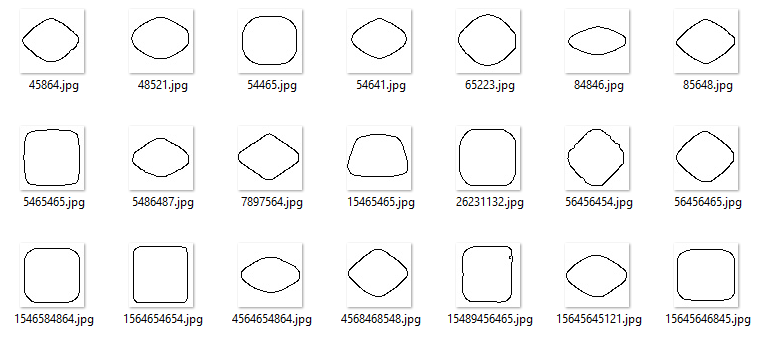
\includegraphics[width=\columnwidth]{Figures/3/opencv1}
				\caption{ตัวอย่างข้อมูลสำหรับการฝึกแบบจำลองรูปทรงสี่เหลี่ยม}
				\label{Fig:opencv1}
			\end{figure}

			\begin{figure}[H]
				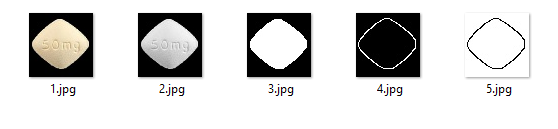
\includegraphics[width=\columnwidth]{Figures/3/opencv2}
				\caption{แสดงการขั้นตอนการทำความสะอาดข้อมูลรูปสำหรับใช้ฝึกและสอน}
				\label{Fig:opencv2}
			\end{figure}
			จากรูปที่ \ref{Fig:opencv1} รูปภาพตัวอย่างข้อมูลสำหรับการฝึกแบบจำลองรูปทรงสี่เหลี่ยม 
			รูปทรงของยารูปทรงสี่เหลี่ยมมีหลายรูปแบบ 
			ได้แก่
			รูปทรงสี่เหลี่ยมขนมเปียกปูน
			รูปทรงสี่เหลี่ยมจัตุรัส
			รูปทรงสี่เหลี่ยมผืนผ้า 
			และรูปทรงสี่เหลี่ยมขนมเปียกปูน จากรูปทรงทั้งหมด คือ รูปทรงสี่เหลี่ยม
			จากรูปที่ \ref{Fig:opencv2} แสดงลำดับการทำความสะอาดข้อมูลรูปภาพก่อนจะใช้ฝึกและสอนรูปแบบจำลอง SVM kNN และ RFC โดยรูปที่ 1.jpg คือรูปภาพต้นฉบับขนาด 64x64 พิกเซล รูปที่ 2.jpg คือรูปภาพสีเทาที่ถูกเป็นแปลงจาก BGR รูปที่ 3.jpg คือรูปที่ถูกปรับ Threshold รูปที่ 4.jpg คือรูปที่ผ่านการตรวจหา Canny Edge และรูปภาพสุดท้ายรูปที่ 5.jpg คือรูปที่ผ่านการสลับบิท ตามลำดับ

			\item การฝึกและทดสอบแบบจำลอง


			การกำหนดค่าพารามิเตอร์ของแบบจำลอง SVM คือ กำหนดชนิดของ kernelType เป็น RBF กำหนดค่า c เป็น 12.5 และ กำหนดค่า gamma เป็น 0.50625
			แสดงดังรูปที่ \ref{Fig:svm-para} 
						
			\begin{figure}[H]
				{\setstretch{1.0}\begin{lstlisting}
const svm = new cv.SVM({
	kernelType: cv.ml.SVM.RBF,
	c: 12.5,
	gamma: 0.50625
});
				\end{lstlisting}}
				\caption{การกำหนดค่าพารามิเตอร์ของแบบจำลอง SVM}
				\label{Fig:svm-para}
			\end{figure}
			
			จากตารางที่ \ref{tab:SVM} 
			จะเห็นได้ว่ารูปทรงที่ใช้ฝึกและทดสอบมี 6 รูปทรง 
			รูปทรงสี่เหลี่ยมจำแนกถูกต้อง 20 รูปภาพ คิดเป็นร้อยละ 100 
			รูปทรงสามเหลี่ยมจำแนกถูกต้อง 19 รูปภาพ คิดเป็นร้อยละ 95 
			รูปทรงวงกลมจำแนกถูกต้อง 19 รูปภาพ คิดเป็นร้อยละ 95 
			รูปทรงแคปซูลจำแนกถูกต้อง 20 รูปภาพ คิดเป็นร้อยละ 100 
			รูปทรงหกเหลี่ยมจำแนกถูกต้อง 18 รูปภาพ คิดเป็นร้อยละ 90 
			รูปทรงแปดเหลี่ยมจำแนกถูกต้อง 17 รูปภาพ คิดเป็นร้อยละ 85 
			
			ดังนั้นการฝึกและทดสอบแบบจำลอง SVM มีความถูกต้องโดยเฉลี่ยร้อยละ 94.17

			% \begin{table}[H]
			% 	\caption{แสดงความถูกต้องของแบบจำลอง SVM}
			% 	\label{tab:SVM}				
			% 	\begin{tabular}{c}
			% 		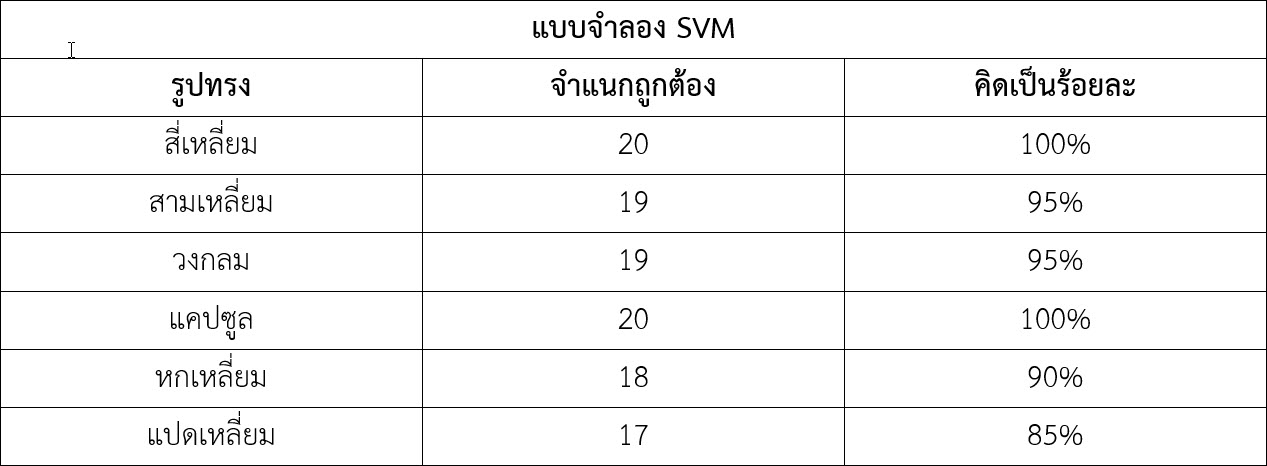
\includegraphics[width=\columnwidth]{Figures/table/SVM}	\\ 
			% 	\end{tabular}
			% \end{table}
			\begin{table}[H]
				\centering
				\caption{แสดงความถูกต้องของแบบจำลอง SVM}
				\label{tab:SVM}
				\begin{tabular}{|p{4cm}|p{4cm}|p{4cm}|}
				\hline
				\multicolumn{1}{|c}{\textbf{รูปทรง}} &
				\multicolumn{1}{|c}{\textbf{จำแนกถูกต้อง}} &
				\multicolumn{1}{|c|}{\textbf{คิดเป็นร้อยละ}} \\ \hline
				\multicolumn{1}{|c}{\textbf{สี่เหลี่ยม}}   & 
				\multicolumn{1}{|c}{\textbf{20}}  &  
				\multicolumn{1}{|c|}{\textbf{100\%}}  \\ \hline
				\multicolumn{1}{|c}{\textbf{สามเหลี่ยม}} & 
				\multicolumn{1}{|c}{\textbf{19}}  &  
				\multicolumn{1}{|c|}{\textbf{95\%}}  \\ \hline
				\multicolumn{1}{|c}{\textbf{วงกลม}}    & 
				\multicolumn{1}{|c}{\textbf{19}}  & 
				\multicolumn{1}{|c|}{\textbf{95\%}}  \\ \hline
				\multicolumn{1}{|c}{\textbf{แคปซูล}}   &  
				\multicolumn{1}{|c}{\textbf{20}} &  
				\multicolumn{1}{|c|}{\textbf{100\%}} \\ \hline
				\multicolumn{1}{|c}{\textbf{หกเหลี่ยม}}  & 
				\multicolumn{1}{|c}{\textbf{18}}  & 
				\multicolumn{1}{|c|}{\textbf{90\%}}   \\ \hline
				\multicolumn{1}{|c}{\textbf{แปดเหลี่ยม}} & 
				\multicolumn{1}{|c}{\textbf{17}}  &  
				\multicolumn{1}{|c|}{\textbf{85\%}}  \\ \hline
				\end{tabular}
			\end{table}
			
			การกำหนดค่าพารามิเตอร์ของแบบจำลอง KNN ดังนี้ 
			train คือ ชุดข้อมูลสำหรับการใช้ฝึกสอนแบบจำลอง 
			cv2.ml.ROW{\_}SAMPLE คือ การกำหนดรูปแบบของชุดข้อมูลเป็นแบบแถว 
			train{\_}labels คือ คลาสของชุดข้อมูลสำหรับการใช้ฝึกสอนแบบจำลอง 
			และ k คือ จำนวนของคลาสที่ใกล้เคียงสูงสุด
			แสดงดังรูปที่  \ref{Fig:knn-para}

			\begin{figure}[H]
				{\setstretch{1.0}\begin{lstlisting}
knn = cv2.ml.KNearest_create()
knn.train(train, cv2.ml.ROW_SAMPLE, train_labels)
result = knn.findNearest(test, k=6)
				\end{lstlisting}}
				\caption{การกำหนดค่าพารามิเตอร์ของแบบจำลอง KNN}
				\label{Fig:knn-para}
			\end{figure}

			จากตารางที่ \ref{tab:KNN}	 การฝึกและทดสอบแบบจำลอง kNN โดยจะเริ่มจากค่า 
			k = 1 ถึง k = 6 จะเห็นได้ว่า 
			K ที่ 1 มีค่าความถูกต้องของแบบจำลองร้อยละ 79.17 
			K ที่ 2 มีค่าความถูกต้องของแบบจำลองร้อยละ 76.67 
			K ที่ 3 มีค่าความถูกต้องของแบบจำลองร้อยละ 74.17 
			K ที่ 4 มีค่าความถูกต้องของแบบจำลองร้อยละ 70.83 
			K ที่ 5 มีค่าความถูกต้องของแบบจำลองร้อยละ 72.50 
			และ K ที่ 6 มีค่าความถูกต้องของแบบจำลองร้อยละ 71.67 

			ดังนั้นการฝึกและทดสอบแบบจำลอง kNN มีความถูกต้องโดยเฉลี่ยร้อยละ 74.17 
			และ K ที่ 1 มีค่าความถูกต้องสูงที่สุดของแบบจำลองร้อยละ 79.17

			% \begin{table}[H]
			% 	\caption{แสดงความถูกต้องของแบบจำลอง kNN}
			% 	\label{tab:KNN}				
			% 	\begin{tabular}{c}
			% 		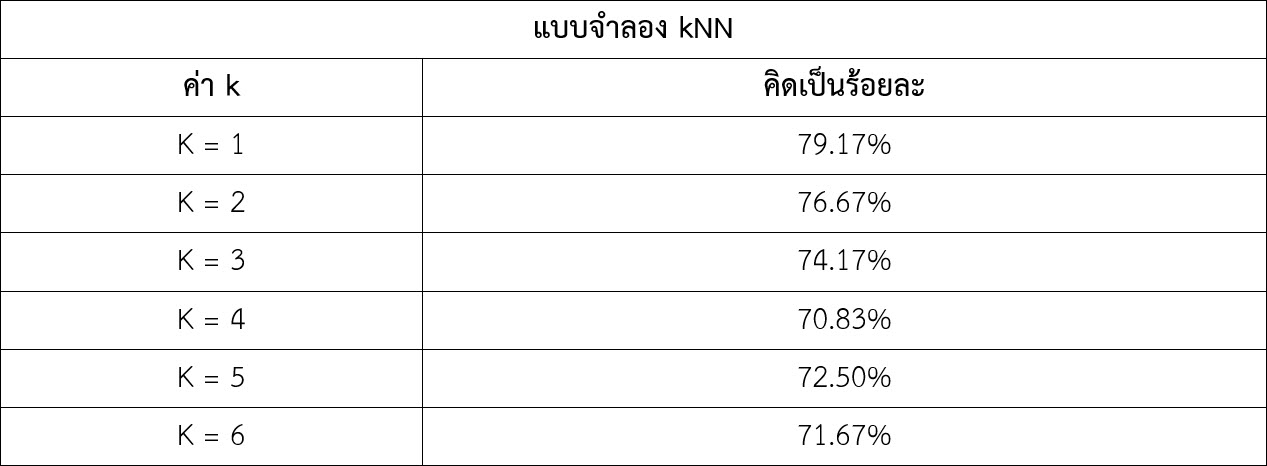
\includegraphics[width=\columnwidth]{Figures/table/KNN}	\\ 
			% 	\end{tabular}
			% \end{table}
			\begin{table}[H]
				\centering
				\caption{แสดงความถูกต้องของแบบจำลอง kNN}
				\label{tab:KNN}
				\begin{tabular}{|c|c|}
				\hline
				ค่า k & คิดเป็นร้อยละ \\ \hline				
				K = 1 &  79.17\% \\ \hline
				K = 2 &  76.67\% \\ \hline
				K = 3 &  74.17\% \\ \hline
				K = 4 &  70.83\% \\ \hline
				K = 5 &  72.50\% \\ \hline
				K = 6 &  71.67\% \\ \hline
				\end{tabular}
			\end{table}

			การกำหนดค่าพารามิเตอร์ของแบบจำลอง KNN 
			โดยการกำหนดพารามิเตอร์ n{\_}estimators คือ จำนวนของต้นไม้ตัดสินใจในการสร้างแบบจำลอง 
			train คือ ชุดข้อมูลสำหรับการใช้ฝึกสอนแบบจำลอง 
			และ train{\_}labels คือ คลาสของชุดข้อมูลสำหรับการใช้ฝึกสอนแบบจำลอง 
			แสดงดังรูปที่ \ref{Fig:rfc-para}

			\begin{figure}[H]
				{\setstretch{1.0}\begin{lstlisting}
RFC = RandomForestClassifier(n_estimators=100)
RFC.fit(train, train_labels)
				\end{lstlisting}}
				\caption{การกำหนดค่าพารามิเตอร์ของแบบจำลอง RFC}
				\label{Fig:rfc-para}
			\end{figure}

			จากตารางที่ \ref{tab:RFC} การฝึกและทดสอบแบบจำลอง RFC 
			โดยมีการปรับค่า {N\_estimators} ตั้งแต่ 10 ถึง 100 
			จะเห็นได้ว่า {N\_estimators} เท่ากับ 10 มีค่าความถูกต้องของแบบจำลองร้อยละ 53.33 
			{N\_estimators} เท่ากับ 30 มีค่าความถูกต้องของแบบจำลองร้อยละ 67.50 
			{N\_estimators} เท่ากับ 50 มีค่าความถูกต้องของแบบจำลองร้อยละ 66.67 
			{N\_estimators} เท่ากับ 70 มีค่าความถูกต้องของแบบจำลองร้อยละ 65.00 
			{N\_estimators} เท่ากับ 90 มีค่าความถูกต้องของแบบจำลองร้อยละ 69.17 
			และ {N\_estimators} เท่ากับ 100 มีค่าความถูกต้องของแบบจำลองร้อยละ 66.67

			ดังนั้นการฝึกและทดสอบแบบจำลอง RFC มีความถูกต้องโดยเฉลี่ยร้อยละ 64.72 และ {N\_estimators} เท่ากับ 90 มีค่าความถูกต้องสูงที่สุดของแบบจำลองร้อยละ 69.17 

			% \begin{table}[H]
			% 	\caption{แสดงความถูกต้องของแบบจำลอง RFC}
			% 	\label{tab:RFC}				
			% 	\begin{tabular}{c}
			% 		\includegraphics[width=\columnwidth]{Figures/table/RFC}	\\ 
			% 	\end{tabular}
			% \end{table}
			\begin{table}[H]
				\centering
				\caption{แสดงความถูกต้องของแบบจำลอง RFC}
				\label{tab:RFC}
				\begin{tabular}{|c|c|}
				\hline
				ค่า N\_estimators & คิดเป็นร้อยละ \\ \hline				
				10 &  53.33\% \\ \hline
				30 &  67.50\% \\ \hline
				50 &  66.67\% \\ \hline
				70 &  65.00\% \\ \hline
				90 &  69.17\% \\ \hline
				100 &  66.67\% \\ \hline
				\end{tabular}
			\end{table}



			\item สรุปผลการทำลอง
			
			
			จากตารางที่ \ref{tab:SVM} \ref{tab:KNN} และ \ref{tab:RFC} 
			จะเห็นได้ว่าแบบจำลอง SVM มีค่าความถูกต้องร้อยละ 94.17 
			ซึ่งมีค่าความถูกต้องมากกว่าแบบจำลอง 
			kNN มีค่าความถูกต้องร้อยละ 79.17
			และแบบจำลอง RFC มีค่าความถูกต้องร้อยละ 69.17 ตามลำดับ 
			
			ดังนั้นผู้พัฒนาจึงเลือกใช้แบบจำลอง SVM 
			ที่มีความถูกต้องในการจำแนกรูปทรงเม็ดยาสูงที่สุด 
			และนำมาใช้เป็นแบบจำลองในโครงงานแอปพลิเคชันค้นหายาเพื่อคุณ

			\begin{table}[H]
				\centering
				\caption{สรุปผลการทดลอง}
				\label{tab:summary}
				\begin{tabular}{| p{5cm}|c|}
				\hline
				\multicolumn{1}{|c|}{\textbf{แบบจำลอง}} & ค่าความถูกต้อง \\ \hline				
				Support vector machines &  94.17\% \\ \hline
				k-Nearest Neighbors &  79.17\% \\ \hline
				Random Forest Classifier &  69.17 \% \\ \hline
				\end{tabular}
			\end{table}

		\end{enumerate}

	\subsection{การหาขนาดด้านยาวของเม็ดยาโดยใช้วัถตุอ้างอิงที่รู้ขนาด}
		การถ่ายรูปภาพเพื่อหาขนาดด้านยาวของเม็ดยาจำเป็นต้องใช้วัถตุอ้างอิงสีดำที่มีขนาดเท่ากับ 11.3 x 7.3 เซนติเมตร หรือเท่ากับการใช้กระดาษ A4 พับครึ่ง 3 ครั้ง จากรูปที่ \ref{Fig:opencv3}2 พื้นที่สีดำคือวัตถุอ้างอิงที่ทราบขนาด และกรอบสีเหลืองคือ Contour ที่ตรวจพบ หน่วยในภาพเป็นหน่วยพิกเซล ดังนั้นสามารถใช้การเทียบบัญญัติไตรยางศ์เพื่อหาขนาดด้านยาวได้ “1 พิกเซล เท่ากับกี่เซนติเมตร”
	
		ถ้าสมมติให้ขนาดของวัถตุอ้างอิงเท่ากับ 146.9 x 94.9 พิกเซล และกรอบสีเหลืองมีขนาดเท่ากับ 40 x 23 พิกเซล และวัถตุอ้างอิงขนาดเท่ากับ 11.3 x 7.3 เซนติเมตร เมื่อ 146.9 พิกเซล เท่ากับ 11.3 เซนติเมตร และ 1 พิกเซล เท่ากับ ( 11.3 / 146.9 ) = 0.0769 เซนติเมตร ดังนั้น 40 พิกเซล เท่ากับ ( 40 x 0.0769 )  = 3.0769 เซนติเมตร 
	
		\begin{figure}[H]
			\includegraphics[width=\columnwidth]{Figures/3/opencv3}
			\caption{แสดงการวัดขนาดวัตถุด้วยการใช้วัตถุอ้างอิง}
			\label{Fig:opencv3}
		\end{figure}
		

	\subsection{การหาลักษณะสีของยาเม็ด}
		จากรูปที่ \ref{Fig:opencv3} สามารถตรวจพบ Contour กรอบสี่เหลี่ยมสีเหลือง และการหาลักษณะสีของยาเม็ดจะได้จากการแบ่งพื้นของกรอบออกเป็น 4 ส่วนเท่ากัน และดึงค่าสี BGR ที่จุดพิกเซลตรงกลางของแต่ละส่วนนำไปเปรียบเทียบกับตารางที่ 3.6.5 สีที่มีอยู่ในฐานข้อมูลพิสูจน์เอกลักษณ์ยาเพื่อหาค่าต่าง
		
		% \begin{table}[H]
		% 	\caption{ตารางแสดงรหัสสีจากฐานข้อมูลพิสูจน์เอกลักษณ์ยาเม็ด}
		% 	\label{tab:color-list}				
		% 	\begin{tabular}{c}
		% 		\includegraphics[width=\columnwidth]{Figures/table/color-list}	\\ 
		% 	\end{tabular}
		% \end{table}
		\begin{table}[H]
			\centering
			\caption{ตารางแสดงรหัสสีจากฐานข้อมูลพิสูจน์เอกลักษณ์ยาเม็ด}
			\label{tab:color-list}
			\begin{tabular}{ | c | c | c | }
			\hline
			\textbf{ลำดับ} &	\textbf{ชื่อสี} & \textbf{รหัสสี}  \\ \hline
			1	&	ขาว		&	\#FFFFFF  \\ \hline
			2	&	แดง		&	\#ea0000  \\ \hline
			3	&	ส้ม		&	 \#fe700e \\ \hline
			4	&	เหลือง	& \#ffe400 \\ \hline
			5	&	ครีม	& \#efeddb \\ \hline
			6	&	เขียว	& \#a8e26a \\ \hline
			7	&	ฟ้า		&	\#4a9fe0 \\ \hline
			8	&	น้ำเงิน   &	  \#120992 \\ \hline  
			9	&	ชมพู	& \#fdb1ef \\ \hline
			10	&	ม่วง	& \#c977db	\\ \hline
			11	&	น้ำตาล	& \#c2924a	\\ \hline
			12	&	เท่า	& \#cccccc	\\ \hline
			13	&   ดำ 	  &   \#000000	\\ \hline
			\end{tabular}
		\end{table}
		







\chapter{การสร้างระบบ}
การสร้างระบบงานเป็นส่วนหนึ่งของการพัฒนาแอปพลิเคชันค้นหายาเพื่อคุณและเว็บเซอร์วิส ซึ่งจะอธิบายการทำงานของแต่ละส่วน ดังนี้
\begin{itemize}
	\item การค้นหายาแบบทั่วไป
  	\item การค้นหายาแบบขั้นสูง
  	\item การถ่ายรูปภาพ
  	\item	การเรียกใช้งานเว็บเซอร์วิส
  	\item	การติดต่อฐานข้อมูลของเว็บเซอร์วิส
  	\item	การสร้างและการตรวจสอบ JSON Web Token
	\item	การถอดรหัสรูปภาพ BASE64
	\item	การ routing ของเว็บเซอร์วิส
  	\item	การประมวลผลภาพ
\end{itemize}

\section{การค้นหายาแบบทั่วไป}

	เมื่อผู้ใช้งานกรอกข้อความในแถบค้นหาทั่วไป 
	ระบบจะร้องขอการค้นหากับเว็บเซอร์วิสและส่งรายการการค้นหากลับมาแสดงที่หน้ารายการค้นหา 
	แสดงดังภาพที่ \ref{Fig:searchGeneral}
	
	\begin{figure}[H]
		{\setstretch{1.0}\begin{lstlisting}
onInput()  {        
	this.offsetStart  =  1;        
	this.offsetEnd  =  20;        
	this.content.resize();        
	if  (this.searchText)  {            
		this.searchProvider.ganeralSearch(this.searchText.trim(),  this.offsetStart,  this.offsetEnd).then(data  =>  {     
			this.drugs  =  data['results'];                
			this.drugsLength  =  data['length'];          
			if  (data['length']  ==  0)  {          
				this.presentToast();          
			}      
		}).catch((error)  =>  {          
			let  alert  =  this.alertCtrl.create({                    
				title: Error,  
				buttons:  ['close']          
			});          
			alert.present();     
		});    
	}   
}		
		\end{lstlisting}}
		\caption{การค้นหายาแบบทั่วไป}
		\label{Fig:searchGeneral}
	\end{figure}
	จากภาพที่ \ref{Fig:searchGeneral} อธิบายการทำงานของการค้นหายาแบบทั่วไป ได้ดังนี้
	\begin{itemize}[label={--}]
		\item บรรทัดที่  2-3 	กำหนดค่าของตัวแปร สำหรับกำหนดช่วงของรายการที่ต้องการ
		\item บรรทัดที่  4	เป็นคำสั่งเพื่อปรับขนาดของหน้า content
		\item บรรทัดที่  5	เป็นเงื่อนไข ถ้าหากตัวแปรว่างหรือไม่เก็บข้อความใดๆ จะไม่มีการเรียกใช้งานเซอร์วิส
		\item บรรทัดที่  6	เป็นการใช้งานคลาส SearchProvider ฟังก์ชัน ganeralSearch เพื่อร้องขอการค้นหากับเว็บเซอร์วิส 
		\item บรรทัดที่  7	เก็บรายการของการค้นหายาเป็นอาเรย์ในตัวแปร
		\item บรรทัดที่  8	เก็บความยาวของรายการการค้นหายาในตัวแปร
		\item บรรทัดที่  9-10	เงื่อนไขใช้ตรวจสอบความยาวของรายการยา ถ้าหากเท่ากับ 0 แสดงว่าไม่พบเจอรายการ และจะแสดงข้อความขึ้นมาบนหน้าจอ
		\item บรรทัดที่  13-17	ถ้าหากการร้องขอรายการค้นหาเกิดข้อผิดพลาด จะแสดงข้อความขึ้นมาบนหน้าจอ
	\end{itemize}

\section{การค้นหายาแบบขั้นสูง}
	เมื่อผู้ใช้งานกรอกรายละเอียดยาจากหน้าค้นหา 
	ระบบจะร้องขอการค้นหากับเว็บเซอร์วิสและส่งรายการการค้นหากลับมาแสดงที่หน้ารายการค้นหา 
	แสดงดังภาพที่ \ref{Fig:searchAdvance}

	\begin{figure}[H]
		{\setstretch{1.0}\begin{lstlisting}
advanceSearch()  {        
	let  params  =  this.advanceModel();        
	let  loading  =  this.loadingCtrl.create({            
		content:   'Searhing...'        
	});        
    loading.present();        
	this.content.resize();        
	this.offsetStart  =  1;        
	this.offsetEnd  =  20;        
	this.searchProvider.advanceSearch(params,  this.offsetStart,  this.offsetEnd).then(data  =>  {          
		this.drugs  =  data['results'];            
		this.drugsLength  =  data['length'];            
		loading.dismiss();            
		if  (data['length']  ==  0)  {                
			this.presentToast();            
		}        
   }).catch((error)  =>  {            
        loading.dismiss();            
        let  alert  =  this.alertCtrl.create({  
            title: Error  
	    });            
	    alert.present();        
	});    
}    
		\end{lstlisting}}
		\caption{การค้นหายาแบบขั้นสูง}
		\label{Fig:searchAdvance}
	\end{figure}
	จากภาพที่ \ref{Fig:searchAdvance} อธิบายการทำงานของการค้นหาแบบขั้นสูง ได้ดังนี้
	\begin{itemize}[label={--}]
		\item บรรทัดที่ 2	กำหนดตัวแปรสำหรับเก็บข้อมูลโมเดลของ
		\item บรรทัดที่ 3-6	แสดงการ loading 
		\item บรรทัดที่ 7	เป็นคำสั่งเพื่อปรับขนาดของหน้า content
		\item บรรทัดที่ 8-9	กำหนดค่าของตัวแปร สำหรับกำหนดช่วงของรายการที่ต้องการ
		\item บรรทัดที่ 10	เป็นการใช้งานคลาส SearchProvider ฟังก์ชัน advanceSearch เพื่อร้องขอการค้นหากับเว็บเซอร์วิส
		\item บรรทัดที่ 11	เก็บรายการของการค้นหายาเป็นอาเรย์ในตัวแปร
		\item บรรทัดที่ 12	เก็บความยาวของรายการการค้นหายาในตัวแปร
		\item บรรทัดที่ 13	ปิดการแสดงการ loading
		\item บรรทัดที่ 14-15	เงื่อนไขใช้ตรวจสอบความยาวของรายการยา ถ้าหากเท่ากับ 0 แสดงว่าไม่พบเจอรายการ และจะแสดงข้อความขึ้นมาบนหน้าจอ
		\item บรรทัดที่ 17-21	ถ้าหากการร้องขอรายการค้นหาเกิดข้อผิดพลาด จะแสดงข้อความขึ้นมาบนหน้าจอ
		
	\end{itemize}


\section{การถ่ายรูปภาพ}
	ในหน้าการถ่ายรูปภาพเพื่อพิสูจน์เอกลักษณ์ยา 
	เมื่อผู้ใช้งานกดเปิดกล้อง 
	ระบบจะทำการเรียกใช้งานไลบรารี่ Camera ของ Cordova 
	เพื่อทำเรียกใช้งานกล้องของอุปกรณ์ 
	แสดงดังภาพที่ \ref{Fig:camera}

	\begin{figure}[H]
		{\setstretch{1.0}\begin{lstlisting}
options:  CameraOptions  =   {        
    quality:  70,  
	destinationType:  this.camera.DestinationType.DATA_URL,  
    encodingType:  this.camera.EncodingType.JPEG,  
    mediaType:  this.camera.MediaType.PICTURE    
}    
takePicture()   {              
    this.camera.getPicture(this.options).then((imageData)   =>   {                      
        this.imagebase64 = 'data:image/jpeg;base64,'   +   imageData;              
    },     (err)   =>   {                      
        console.log(err);              
    });      
}      
		\end{lstlisting}}
		\caption{การถ่ายรูปภาพ}
		\label{Fig:camera}
	\end{figure}
	จากภาพที่ \ref{Fig:camera} อธิบายการทำงานของการถ่ายรูปภาพ ได้ดังนี้
	\begin{itemize}[label={--}]
		\item บรรทัดที่ 1-6	กำหนด options ของการถ่ายรูป คุณภาพของรูป ชนิดของรูปภาพ 
		\item บรรทัดที่ 7-13	เป็นฟังก์ชันการถ่ายรูปภาพ เมื่อการถ่ายรูปสำเร็จ รูปภาพจะถูกเก็บในรูปแบบ base64 ในตัวแปรชื่อ imagebase64
		\item บรรทัดที่ 8	เปิดการทำงานของกล้องถ่ายรูปบนอุปกรณ์
		\item บรรทัดที่ 9 	กำหนดตัวแปร imagebase64 สำหรับเก็บรูปภาพในรูปแบบ base64 ที่ได้จากการถ่ายรูป
	\end{itemize}

\section{การเรียกใช้งานเว็บเซอร์วิส}
	การเรียกใช้งานเว็บเซอร์วิสด้วยการใช้ไลบรารี HTTP ของ Cordova 
	แสดงดังภาพที่ \ref{Fig:callService}

	\begin{figure}[H]
		{\setstretch{1.0}\begin{lstlisting}
setOption()  {        
    let  headers  =  new  Headers;        
    headers.set('api-key',  this.apiToken);        
    headers.append('Content-type',  'application/json')  this.opt  =  new  RequestOptions({            
        headers:  headers        
    });    
}    
ganeralSearch(input:  string,  offsetStart:  any,  offsetEnd:  any)  {        
    if  (offsetStart  ==  -1  ||  offsetEnd  ==  -1)  {            
	    offsetStart  =  1,  offsetEnd  =  10;        
	}        
	return  new  Promise((resolve,  reject)  =>  {            
		this.http.get(`${this.apiEndPoint}/drugs/search?input=${input}&offsetStart=${offsetStart}&offsetEnd=${offsetEnd}`,  this.opt).map(res  =>  res.json()).subscribe(data  =>  {                
			resolve(data);            
		},  error  =>  {                
			reject(error);            
		});        
    });    
}    
		\end{lstlisting}}
		\caption{การเรียกใช้งานเว็บเซอร์วิสs}
		\label{Fig:callService}
	\end{figure}
	จากภาพที่ \ref{Fig:callService} อธิบายการทำงานของการใช้งานเว็บเซอร์วิส ได้ดังนี้
	
	\begin{itemize}[label={--}]
		\item บรรทัดที่ 1-7	เป็นฟังก์ชันการกำหนดค่าเริ่มต้นของ Header โดยจะกำหนดรูปแบบและส่ง api-token 
		\item บรรทัดที่ 8-19	เป็นฟังก์ชันสำหรับติดต่อกับเว็บเซอร์วิส โดยยกตัวอย่างการค้นหาแบบทั่วไป
		\item บรรทัดที่ 12-17	เป็นการเรียกใช้งาน HTTP แบบ GET จะร้องขอไปที่อยู่ (URL) ของเว็บเซอร์วิส
		
	\end{itemize}

\section{การติดต่อฐานข้อมูลของเว็บเซอร์วิส}
	การติดต่อกับฐานข้อมูลการพิสูจน์เอกลักษณํยาเม็ดหรือแคปซูลของคณะเภสัชศาสตร์ มหาวิทยาวัยอุบลราชธานี 
	ใช้ไลบรารี่ของ nodejs ชื่อ mysql 
	แสดงดังภาพที่ \ref{Fig:connectDB}

	\begin{figure}[H]
		{\setstretch{1.0}\begin{lstlisting}
const  mysql  =  require('mysql');    
const  configDB  =  require('./config');    
var  pool  =  mysql.createPool(configDB.info);    
pool.getConnection(function(err,  connection)  {        
	if  (err)  throw  err;        
	console.log('Connected',  new  Date());    
});    
		\end{lstlisting}}
		\caption{การติดต่อฐานข้อมูลของเว็บเซอร์วิส}
		\label{Fig:connectDB}
	\end{figure}
	จากภาพที่ \ref{Fig:connectDB} อธิบายการทำงานของการติดต่อฐานข้อมูลของเว็บเซอร์วิส ได้ดังนี้
	\begin{itemize}[label={--}]
		\item บรรทัดที่ 1	กำหนดตัวแปรชื่อ mysql สำหรับเก็บไลบรารีชื่อว่า mysql
		\item บรรทัดที่ 2	กำหนดตัวแปรชื่อ configDB สำหรับเก็บข้อมูลการ key-value เพื่อใช้ติดต่อกับฐานข้อมูล
		\item บรรทัดที่ 3	กำหนดตัวแปรชื่อ pool สำหรับเก็บข้อมูลการสร้างการเชื่อมต่อกับฐานข้อมูล
		\item บรรทัดที่ 4-7	เป็นการเรียกใช้งานฟังก์ชันชื่อว่า getConnection เพื่อติดต่อกับฐานข้อมูล 
	\end{itemize}


\section{การสร้างและการตรวจสอบ JSON Web Token}
	นำ JSON Web Token มาช่วยในการระบุตัวตนก่อนให้ใช้งานกับเว็บเซอร์วิส 
	โดยใช้ไลบรารี่ของ nodejs ชื่อว่า jsonwebtoken 
	แสดงดังภาพที่ \ref{Fig:jsonwebtokenMaker}
	\begin{figure}[H]
		{\setstretch{1.0}\begin{lstlisting}
var  jwt  =  require('jsonwebtoken');    
var  fs  =  require('fs');    
const  uuid  =  require('uuid/v4');    
module.exports  =   {        
	sign:   function(req,  res,  next)  {            
		var  data  =   {                
			id:  req.query.id,  
			uuid:  uuid()            
		};            
		var  cert  =  fs.readFileSync('./auth/keys/private.key');            
		jwt.sign(data,  cert,   {                
			algorithm:   'RS256',  
			expiresIn:   "120d"            
		},  function(err,  token)  {                
			if  (err)  {                    
				console.log('Token error ',  err.message);                    
				return  res.status(405).send({                        
					err:  err                    
				});                
			}                
			req.query.token  =  token;                
			return  res.status(200).send({                    
				token:  req.query.token                
			});            
		});        
	},verify:   function(req,  res,  next)  {            
		var  cert  =  fs.readFileSync('./auth/keys/public.pem');            
		jwt.verify(req.headers['api-key'],  cert,   {                
			algorithms:  ['RS256']            
		},  function(err,  payload)  {                
			if  (err)  {                    
				return  res.status(401).send({                        
					err:  err                    
				});                
			}                
			req.query.payload  =  payload;                
			next();           
		});        
	}  
};    
		\end{lstlisting}}
		\caption{การสร้างและการตรวจสอบ JSON Web Token}
		\label{Fig:jsonwebtokenMaker}
	\end{figure}
	จากภาพที่ \ref{Fig:jsonwebtokenMaker} อธิบายการทำงานของการสร้างและการตรวจสอบ JSON Web Token ได้ดังนี้
	\begin{itemize}[label={--}]
		\item บรรทัดที่ 1	กำหนดตัวแปรชื่อ jwt สำหรับเรียกใช้งานไลบารีชื่อว่า jsonwebtoken 
		\item บรรทัดที่ 2	กำหนดตัวแปรชื่อ js สำหรับเรียกใช้งานไลบารีชื่อว่า js เพื่อการเขียนไฟล์
		\item บรรทัดที่ 5-26	เป็นฟังก์ชันการสร้าง jwt โดยจะใช้ fs อ่านไฟล์ชื่อว่า private.pem เพื่อใช้สำหรับการเข้ารหัส กำหนดรูปแบบและอายุการใช้งานของ jwt
		\item บรรทัดที่ 27-40	เป็นฟังก์ชันการตรวจสอบความถูกต้องของ jwt โดยจะใช้ fs อ่านไฟล์ชื่อว่า public.pem เพื่อใช้สำหรับการถอดรหัสและตรวจสอบ jwt
	\end{itemize}


\section{การถอดรหัสรูปภาพ BASE64}
	ในการส่งรูปภาพจากเครื่องผู้ใช้งานมายังเว็บเซอร์วิส 
	จะถูกส่งรูปภาพมาในรูปแบบ base64 
	แสดงดังรูปภาพที่ \ref{Fig:decodeBase64}

	\begin{figure}[H]
		{\setstretch{1.0}\begin{lstlisting}
var  fs  =  require('fs');    
const  uuid  =  require('uuid/v4');    
module.exports  =   {        
	decode64:   function(req,  res,  next)  {            
		var  body  =  req.body;            
		var  base64Data  =  body.imageBase64.replace(/^data:image\/jpeg;base64,/,  "");            
		let  filename  =  `${uuid()}.jpeg`;            
		let  filePath  =  `./assets/images/${filename}`;            
		fs.writeFile(filePath,  base64Data,  'base64',  function(err)  {                
			if  (err)  {                    
				console.log('Error ',  err.message);                    
				return  res.status(500).send(err.message);                
			}                
			req.query.filename  =  filename;                
			req.query.filePath  =  filePath;                
			console.log(req.query.filePath);                
			next();            
		});       
	}    
};    
		\end{lstlisting}}
		\caption{การถอดรหัสรูปภาพ BASE64}
		\label{Fig:decodeBase64}
	\end{figure}
	จากภาพที่ \ref{Fig:decodeBase64} อธิบายการทำงานของการถอดรหัสรูปภาพ BASE64 ได้ดังนี้
	\begin{itemize}[label={--}]
		\item บรรทัดที่ 1	กำหนดตัวแปรชื่อ js สำหรับเรียกใช้งานไลบารีชื่อว่า js เพื่อการเขียนไฟล์
		\item บรรทัดที่ 2	กำหนดตัวแปรชื่อ uuid สำหรับเรียกใช้งานไลบารีชื่อว่า uuid/v4 เพื่อการสร้างชื่อไฟล์
		\item บรรทัดที่ 4-19	เป็นฟังก์ชันการถอดรหัสรูปภาพ BASE64
		\item บรรทัดที่ 5	กำหนดตัวแปรชื่อ body สำหรับเก็บค่าจาก req.body
		\item บรรทัดที่ 6	กำหนดตัวแปรชื่อ base64Data สำหรับเก็บข้อมูลรูปภาพจาก body 
		\item บรรทัดที่ 7	กำหนดตัวแปรชื่อ filename สำหรับเก็บชื่อไฟล์ภาพ จากการเรียกใช้งานฟังก์ชัน uuid ของไลบรารี่ uuid/v4
		\item บรรทัดที่ 9 	เรียกใช้งานฟังก์ชัน writeFile จาก fs สำหรับการเขียนไฟล์
		\item บรรทัดที่ 14-15	เก็บค่า filename กับ filePate ไว้ใน req.query
		\item บรรทัดที่ 17	เรียกฟังก์ชัน next() เพื่อทำงานฟังก์ชันต่อไป
	\end{itemize}

\section{การ routing ของเว็บเซอร์วิส}
การ routing ของเว็บเซอร์วิสใช้ไบรารี่ของ nodejs ชื่อ express 
สำหรับเป็นเว็บเซอร์วิสติดต่อกับฐานข้อมูลและประมวลผลภาพ 
แสดงดังภาพที่ \ref{Fig:expressRouting}

	\begin{figure}[H]
		{\setstretch{1.0}\begin{lstlisting}
var   app   =   require('express')();      
var   bodyParser   =   require('body-parser');      
var   cors   =   require('cors');      
var   POST   =   process.env.PORT   ||   5000;    
var   con   =   require('./db/connectDB')   
var   jwt   =   require('./auth/auth');      
var   decode64   =   require('./base64/base64');     
var   opencv    =    require('./openCV/svmTest');        
app.use(bodyParser.json({              
	limit:     '5mb'      
}));      
app.use(bodyParser.urlencoded({              
	limit:     '5mb',  
	extended:   true      
}));      
app.use(cors());      
app.use('/drugs',   jwt.verify,   con.checkAuth);    
app.get('/token/sign',   jwt.sign);      
app.get('/token/verify',   jwt.verify,   jwt.verified);    
app.get('/drugs/id',   con.getDrug);      
app.get('/drugs/search',   con.genaralSearchDrugs);      
app.get('/drugs/search/advance',   con.advanceSearchDrugs);      
app.get('/drugs/dimg',   con.getDimg);      
app.get('/drugs/bookmarks',   con.getBookmarks)  
app.get('/ddl/color',   con.ddlColor);      
app.get('/ddl/dgroup',   con.ddlDgroup);      
app.get('/ddl/drtype',   con.ddlDrtype);      
app.get('/ddl/dshape',   con.ddlDshape);      
app.get('/ddl/dsize',   con.ddlDsize);      
app.get('/ddl/dstatus',   con.ddlDstatus);      
app.get('/ddl/dtype',   con.ddlDtype);      
app.get('/ddl/shapetype',    con.ddlShapetype);      
app.post('/api/drugs/upload',   decode64.decode64,   opencv.getSizeAndColors,   opencv.predict);      
var   server   =   app.listen(POST,   function()   {              
	console.log('express is running on port:'   +   POST);      
});      
		\end{lstlisting}}
		\caption{การ routing ของเว็บเซอร์วิส}
		\label{Fig:expressRouting}
	\end{figure}
	จากภาพที่ \ref{Fig:expressRouting} อธิบายการทำงานของการ routing ของเว็บเซอร์วิส ได้ดังนี้
	\begin{itemize}[label={--}]
		\item บรรทัดที่ 1	เรียกใช้งานไลบรารี Express และเก็บไว้ในตัวแปรชื่อ app เป็นไลบรารีหลักในการทำงานของ Web application framework
		\item บรรทัดที่ 2	เรียกใช้งานไลบรารี bodyparser และเก็บไว้ในตัวแปรชื่อ bodyparser เป็น Middleware ทำหน้าที่เป็นตัวกรอง requeset 
		\item บรรทัดที่ 3	เรียกใช้งานไลบรารี cors และเก็บไว้ในตัวแปรชื่อ cors เป็นกลไลที่ทำให้เว็บเซอร์วิสสามารถอนุญาตการร้องขอทรัพยากรจากเครื่องผู้ใช้งาน
		\item บรรทัดที่ 4	กำหนดตัวแปรชื่อ PORT 
		\item บรรทัดที่ 5	เรียกใช้งานการเชื่อมต่อกับฐานข้อมูล เก็บไว้ในตัวแปรชื่อ 
		\item บรรทัดที่ 6	เรียกใช้งานการจัดการ JSON web token เก็บไว้ในตัวแปรชื่อ jwt
		\item บรรทัดที่ 4	เรียกใช้งานการถอดรหัสรูปภาพ base64 เก็บไว้ในตัวแปรชื่อ decode64
		\item บรรทัดที่ 8-15	กำหนดค่าของเริ่มต้นของ Middleware
		\item บรรทัดที่ 16	กำหนดการ routing เพื่อตรวจสอบการร้องขอก่อนจะให้เรียกทรัพยากร ด้วยการตรวจสอบ JWT ที่ส่งมาด้วยกับ HTTP Request 
		\item บรรทัดที่ 18	กำหนดการ routing สำหรับการจ้องขอเพื่อขอ JWT 
		\item บรรทัดที่ 19	กำหนดการ routing สำหรับการตรวจสอบ JWT
		\item บรรทัดที่ 20	กำหนดการ routing สำหรับการร้องขอทรัพยากรรายการยาแบบละเอียด
		\item บรรทัดที่ 21	กำหนดการ routing สำหรับการร้องขอทรัพยากรแบบการค้นหายาทั่วไป
		\item บรรทัดที่ 22	กำหนดการ routing สำหรับการร้องขอทรัพยากรแบบการค้นหายาขั้นสูง
		\item บรรทัดที่ 23	กำหนดการ routing สำหรับการร้องขอทรัพยากรรายการรูปภาพของยา
		\item บรรทัดที่ 24	กำหนดการ routing สำหรับการร้องขอทรัพยากรรายการยาที่ผู้ใช้งานบุ๊กมาร์กไว้ที่เครื่อง
		\item บรรทัดที่ 25	กำหนดการ routing สำหรับการร้องขอทรัพยากรรายการ Dropdownlist ลักษณะสีของยา
		\item บรรทัดที่ 26	กำหนดการ routing สำหรับการร้องขอทรัพยากรรายการ Dropdownlist ประเภททะเบียนยา
		\item บรรทัดที่ 27	กำหนดการ routing สำหรับการร้องขอทรัพยากรรายการ Dropdownlist รูปแบบผลิตภัณฑ์
		\item บรรทัดที่ 28	กำหนดการ routing สำหรับการร้องขอทรัพยากรรายการ Dropdownlist สัญลักษณ์ที่ปรากฏบนเม็ดยา
		\item บรรทัดที่ 29	กำหนดการ routing สำหรับการร้องขอทรัพยากรรายการ Dropdownlist ขนาดของยา
		\item บรรทัดที่ 30	กำหนดการ routing สำหรับการร้องขอทรัพยากรรายการ Dropdownlist สถานะของยา
		\item บรรทัดที่ 31	กำหนดการ routing สำหรับการร้องขอทรัพยากรรายการ Dropdownlist รูปร่างลักษณะยา
		\item บรรทัดที่ 32	กำหนดการ routing สำหรับการร้องขอทรัพยากรรายการ Dropdownlist ของรูปทรงยา
		\item บรรทัดที่ 33	กำหนดการ routing สำหรับการร้องขอเพื่อส่งรูปภาพยามาที่เว็บเซอร์วิสเพื่อประมวลผลรูปภาพยา
		\item บรรทัดที่ 34-36	ให้เว็บเซอร์วิสทำงานที่ PORT ที่ถูกกำหนดไว้
	\end{itemize}
	

\section{การประมวลผลภาพ}
	การประมวลภาพรูปภาพใช้ไลบรารีของ nodejs ชื่อ opencv4nodejs 
	แสดงดังภาพที่ \ref{Fig:imageProcessing1}

	\begin{figure}[H]
		{\setstretch{1.0}\begin{lstlisting}\ContinueLineNumber
predict:   function(req,  res,  next)  {        
    let  testDataPath  =  `./src/assets/threshold/${req.query.filename}`;        
    let  img  =  cv.imread(testDataPath);        
    img  =  img.resize(64,  64);        
    try  {            
        const  desc  =  computeHOGDescriptorFromImage(img,  false);            
        if  (!desc)  {                
            throw  new  Error(`Computing HOG descriptor failed for file: ${file}`);            
        }            
        let  svmPredict  =  svm.predict(desc);            
        let  dshape  =   [];            
        let  predict  =   {                
            label:  lccs[svmPredict],  
            colors:  req.query.colors,  
			colorid:  req.query.colorid,  
			colorname:  req.query.colorname,  
			width:  req.query.width,  
			dshape:  lccs[svmPredict]]            
        }            
        return  res.status(200).send(predict);        
    }   
		\end{lstlisting}}
		\caption{การประมวลผลภาพ}
		\label{Fig:imageProcessing1}
	\end{figure}
	\begin{figure}[H]
		{\setstretch{1.0}\begin{lstlisting}\ContinueLineNumber
	catch  (err)  {            
		return  res.status(200).send({                
			isError:  true,  
			messages:  err            
		});        
	}},  getSizeAndColors:   function(req,  res,  next)  {        
	let  testDataPath  =  `./src/assets/images/${req.query.filename}`;        
	let  mat  =  cv.imread(testDataPath);        
	mat  =  mat.resize(1024,  1024);        
	const  know_width  =  11.3       
	const  know_heigth  =  7.3       
	let  boundingRect  =   [];        
	let  num  =  0;        
	const  thd  =  1500;        
	const  threshold  =  100;        
	const  matGray  =  mat.bgrToGray();        
	var  thresh  =  matGray.threshold(100,  255,  0);    
	const  contours  =  thresh.findContours(cv.RETR_CCOMP,  cv.CHAIN_APPROX_SIMPLE,  new  cv.Point(0,  0));        
try  {            
	for  (let  i  =  0;  i  <  contours.length;  i++)  {                
		var  brect  =  contours[i].boundingRect();                
		const  pt1  =  new  cv.Point(brect.x,  brect.y);                
		const  pt2  =  new  cv.Point(brect.x  +  brect.width,  brect.y  +  brect.height);                
		if  (brect.width  *  brect.height  >=  thd)  {                    
			boundingRect.push(brect);                    
			num++;                    
			mat.drawRectangle(pt2,  pt1,  blue);                    
			const  region  =  mat.getRegion(brect);               
		}   
		else  {                    
			mat.drawRectangle(pt2,  pt1,  red);                
		}            
	}           
	var  matThresh  =  mat.threshold(100,  255,  0);           
	\end{lstlisting}}
	\caption{การประมวลผลภาพ(ต่อ)}
	\label{Fig:imageProcessing2}
	\end{figure}

	\begin{figure}[H]
		{\setstretch{1.0}\begin{lstlisting}\ContinueLineNumber
	if  (num  <  2)  {                
		return  res.send({                    
			isError:  true,  
			messages:   'contounrs < 2.'                
		});            
	}            
	boundingRect.sort(function(rect1,  rect2)  {                
		if  (rect1.height  +  rect1.width  >  rect2.height  +  rect2.width)  {                    
			return  1;                
		}            
	});            
	const  padding  =  5;            
	const  newRect  =  new  cv.Rect((boundingRect[0].x  -  padding)  >=  0  ?  boundingRect[0].x  -  padding  :  0,   (boundingRect[0].y  -  padding)  >=  0  ?  boundingRect[0].y  -  padding  :  0,  mat.cols  -  (boundingRect[0].x  +  boundingRect[0].width  +  padding  *  2)  >=  0  ?  (boundingRect[0].width  +  padding  *  2)  :  boundingRect[0].width,  mat.rows  -  (boundingRect[0].y  +  boundingRect[0].height  +  padding  *  2)  >=  0  ?  (boundingRect[0].height  +  padding  *  2)  :  boundingRect[0].height);
	const  region  =  thresh.getRegion(newRect);            
	var  cols  =  region.cols;            
	var  rows  =  region.rows;            
	var  pad  =  0;            
	if  (region.cols  >  region.rows)  {                
		pad  =  region.cols  -  region.rows;                
		rows  +=  pad;            
	}   
	else  {                
		pad  =  region.rows  -  region.cols;                
		cols  +=  pad;            
	}            
	var  matPadded  =  new  cv.Mat(rows,  cols,  cv.CV_8UC1,  0);            
	for  (let  i  =  0;  i  <  region.rows;  i++)  {                
		for  (let  j  =  0;  j  <  region.cols;  j++)  {                    
			let  atMat  =  region.at(i,  j);                    
			if  (region.cols  >  region.rows)  {                        
				matPadded.set(i  +  (pad  /  2),  j,  atMat);                    
			}   
		\end{lstlisting}}
		\caption{การประมวลผลภาพ(ต่อ)}
		\label{Fig:imageProcessing2}
	\end{figure}

	\begin{figure}[H]
		{\setstretch{1.0}\begin{lstlisting}\ContinueLineNumber
			else  {                        
				matPadded.set(i,  j  +  (pad  /  2),  atMat);                    
			}                
		}            
	}            
	matPadded  =  matPadded.resize(64,  64);            
	let  matCanny  =  matPadded.canny(threshold,  threshold,  3,  true);            
	let  matInvert  =  matCanny.bitwiseNot();            
	cv.imwrite(`./src/assets/threshold/${req.query.filename}`,  matInvert);           
	var  point  =   [];            
	var  colors  =   [];            
		var  colorid  =   [];            
		var  colorname  =   [];            
	let  hexColors  =   ['FFFFFF',  'ea0000',  'fe700e',  'ffe400',  'efeddb',  'a8e26a',  '4a9fe0',  '120992',  'fdb1ef',  'c977db',  'c2924a',  'cccccc',  '000000']            
	let  nameColors  =   [];     
	point.push([boundingRect[0].x  +  (boundingRect[0].width  /  4),  boundingRect[0].y  +  (boundingRect[0].height  /  4)]);            
	point.push([boundingRect[0].x  +  (boundingRect[0].width  /  4),  boundingRect[0].y  +  (boundingRect[0].height  *  3  /  4)]);            
	point.push([boundingRect[0].x  +  (boundingRect[0].width  *  3  /  4),  boundingRect[0].y  +  (boundingRect[0].height  /  4)]);            
	point.push([boundingRect[0].x  +  (boundingRect[0].width  *  3  /  4),  boundingRect[0].y  +  (boundingRect[0].height  *  3  /  4)]);            
	for  (let  i  =  0;  i  <  4;  i++)  {                
		let  bgr  =  matThresh.atRaw(parseInt(point[i][1]),  parseInt(point[i][0]));                
		let  diffColor  =  101;                
		let  indexColor  =  0;                
		let  hexColor  =  rgbHex(bgr[2],  bgr[1],  bgr[0]); 
	 	\end{lstlisting}}
		\caption{การประมวลผลภาพ(ต่อ)}
		\label{Fig:imageProcessing3}
	\end{figure}
	\begin{figure}[H]
		{\setstretch{1.0}\begin{lstlisting}
		for  (let  j  =  0;  j  <  hexColors.length;  j++)  {                    
			let  tmp  =  cd.compare(hexColor,  hexColors[j]);                    
			if  (tmp  <  diffColor)  {                        
				diffColor  =  tmp;                        
				indexColor  =  j;                    
			}                
		}                
		if  (!colorid.includes(indexColor  +  1))  {                    
			colors.push(hexColors[indexColor]);                    
			colorid.push(indexColor  +  1);                    
			colorname.push(nameColors[indexColor]);                
		}            
	}            
	const  Rwidth  =  boundingRect[1].width  <  boundingRect[1].height  ?  boundingRect[1].height  :  boundingRect[1].width;            
	const  Owidth  =  boundingRect[0].width  <  boundingRect[0].height  ?  boundingRect[0].height  :  boundingRect[0].width;            
	const  width  =   (know_width  /  Rwidth)  *  Owidth;            
	req.query.colors  =  colors;            
	req.query.colorid  =  colorid;            
	req.query.colorname  =  colorname;            
	req.query.boundingRect  =  boundingRect[0];            
	req.query.width  =  width;            
	next();        
	}   
	catch  (err)  {            
		return  res.status(200).send({                
			isError:  true,  
			messages:  err            
		});        
	}    
}   
	 	\end{lstlisting}}
		\caption{การประมวลผลภาพ(ต่อ)}
		\label{Fig:imageProcessing4}
	\end{figure}
	จากภาพที่ \ref{Fig:imageProcessing1} อธิบายการทำงานของการประมวลผลภาพ ได้ดังนี้
	\begin{itemize}[label={--}]
		\item บรรทัดที่ 1-26	ฟังก์ชันการจำแนกรูปทรงของยา
		\item บรรทัดที่ 27-137 ฟังก์ชันสำหรับการประมวลผลภาพเพื่อหาขนาดและสีของเม็ดยา
		\item บรรทัดที่ 2-3	กำหนด path และอ่านไฟล์มาเก็บในตัวแปร img
		\item บรรทัดที่ 4	ปรับขนาดของรูปภาพเป็นขนาด 64x64 พิกเซล
		\item บรรทัดที่ 6-9	เรียกฟังก์ชันสำหรับการแปรงรูปภาพให้เป็นอาเรย์ เพื่อที่จะนำไปจำแนกรูปทรง
		\item บรรทัดที่ 10	เรียกฟังก์ชันเพื่อจำแนกรูปทรงของยาและเก็บที่ตัวแปรชื่อว่า svmPredict
		\item บรรทัดที่ 11	กำหนดตัวชื่อ dshape เป็น label ของรูปทรงต่างๆ 
		\item บรรทัดที่ 12-19	กำหนดตัวชื่อ predict สำหรับเก็บผลลัพธ์การประมวลผล
		\item บรรทัดที่ 20	คืนผลลัพธ์กลับไปที่เครื่องผู้ใช้งาน
		\item บรรทัดที่ 28-29 กำหนด path และอ่านไฟล์มาเก็บในตัวแปร mat
		\item บรรทัดที่ 31-32 กำหนดขนาดด้านยาวและด้านกว้างของวัตถุอ้างอิง ในตัวแปรชื่อ {know\_width} และ {know\_height}
		\item บรรทัดที่ 33	กำหนดตัวแปรชื่อว่า boundingRect สำหรับเก็บ Contounr
		\item บรรทัดที่ 35	กำหนดตัวแปรชื่อ thd เก็บค่า threshold เพื่อค่าขั้นต่ำของขนาด Contounr 
		\item บรรทัดที่ 36	กำหนดตัวแปรชื่อ threshold เก็บค่า threshold ของการปรับภาพให้เป็น Canny Edge
		\item บรรทัดที่ 37	ปรับภาพเป็นให้ภาพ Grayscale
		\item บรรทัดที่ 38	ปรับ threshold ของภาพ Grayscale
		\item บรรทัดที่ 39	นำภาพจากตัวแปร thresh มาหา Contounrs ด้วยฟังก์ชัน fildContounrs 
		\item บรรทัดที่ 41-53	ตรวจหา contounr ที่เป็นวัถตุอ้างอิงและวัตถุเป้าหมาย (ยา) และเก็บในอาเรย์ชื่อ boundingRect 
		\item บรรทัดที่ 55-59	ถ้าหากมี contounr เพียง 0 – 1 อัน จะไม่สามารถดำเนินการต่อไปได้ และคืนข้อผิดพลาดกลับไปที่เครื่องผู้ใช้งาน
		\item บรรทัดที่ 61-63	เป็นการเรียงลำดับขนาดพิ้นที่ของ contounr จากน้อยไปมาก 
		\item บรรทัดที่ 66-89 เป็นการตัดภาพเอาเฉพาะภาพยาเม็ด และปรับภาพให้เป็นสี่เหลี่ยมจัตุรัส
		\item บรรทัดที่ 91-93 นำภาพเม็ดยามาหา Canny Edge และเขียนไฟล์รูปภาพ
		\item บรรทัดที่ 94 	กำหนดตัวแปรชื่อ point สำหรับการเก็บตำแหน่งของสีของภาพเม็ดยา 
		\item บรรทัดที่ 95-97	กำหนดตัวแปรชื่อ colors colored และ colorname สำหรับเก็บข้อมูลของสี
		\item บรรทัดที่ 98	กำหนดตัวแปรชื่อ hexColors สำหรับเก็บค่าโค้ดสีจากฐานข้อมูล
		\item บรรทัดที่ 99	กำหนดตัวแปรชื่อ nameColors สำหรับชื่อสีจากฐานข้อมูล
		\item บรรทัดที่ 100-120 เป็นการดึงค่าสี BGR จากภาพยาเม็ดด้วยตำแหน่งที่ได้อาเรย์ชื่อ point และนำค่าสีไปเปรียบเทียบกับอาเรย์ชื่อ hexColor เพื่อหาค่าสีที่ใกล้เคียงกันมากที่สุด
		\item บรรทัดที่ 122-124 เป็นการวัดขนาดด้านยาวของเม็ดยา โดยใช้การอ้างอิงจากวัตถุที่รู้ขนาดอยู่แล้ว
		\item บรรทัดที่ 125-129 เก็บผลลัพธ์การพิสูจน์เอกลักษณ์ยาเม็ด ไว้ใน req.query 
		\item บรรทัดที่ 130	เรียกฟังก์ชัน next() เพื่อทำงานฟังก์ชันต่อไป
		\item บรรทัดที่ 131-135 ถ้าหากการประมวลผลภาพเกิดข้อผิดพลาด จะทำการส่งข้อความบอกข้อผิดพลาดไปที่เครื่องผู้ใช้งาน
	\end{itemize}


\chapter{การทดสอบระบบ}
ขั้นตอนการทดสอบระบบงานถือเป็นขั้นตอนหนึ่งที่สำคัญของการสร้างระบบงานเนื่องจากเป็นการสรุปงานหรือเพื่อดูประสิทธิภาพของการพัฒนาระบบงานรวมทั้งทำให้ทราบถึงปัญหาที่อาจเกิดขึ้นก่อนที่จะนำระบบงานไปใช้งานจริง เพื่อทำการแก้ไขปัญหาได้ทันท่วงที ทั้งนี้เพื่อให้การพัฒนาระบบงานมีความสมบูรณ์มากที่สุด ทำให้เกิดประโยชน์ต่อผู้ใช้งาน และผู้พัฒนาระบบต่อไป แอปพลิเคชันค้นหายาเพื่อคุณที่ได้พัฒนาขึ้นนี้ 
ได้มีการทดสอบระบบงานในส่วนต่างๆ ดังนี้
\begin{itemize}[label={--}]
	\item ผลการทดสอบการค้นหายาแบบทั่วไป
	\item ผลการทดสอบการค้นหายาแบบขั้นสูง
	\item ผลการทดสอบเลือกดูรายละเอียดยา
	\item ผลการทดสอบถ่ายรูปภาพเพื่อการพิสูจน์เอกลักษณ์ยาเม็ด
	\item ผลการทดสอบการ rounting ของเว็บเซอร์วิส
\end{itemize}

\section{ผลการทดสอบการค้นหายาแบบทั่วไป}
% \begin{table}[H]
% 	\caption{ผลการทดสอบค้นหายาแบบทั่วไป}
% 	\label{tab:test1}
% 	\begin{tabular}{c}
% 		\includegraphics[width=\columnwidth]{Figures/table/test1}	\\ 
% 	\end{tabular}
% \end{table}
\begin{table}[H]
	\caption{ผลการทดสอบค้นหายาแบบทั่วไป}
    \centering	
	\label{tab:test1}
    \begin{tabular}{ | p{4.5cm} | p{4.5cm} | p{4.5cm} | }
    \hline
	% {\setstretch{1.0} } 
	การทำงาน & เงื่อนไขการทดสอบ & ผลการทดสอบ \\ \hline
	\setstretch{1.0}{ทดสอบการค้นหาแบบทั่วไป 
	& \setstretch{1.0}{ไม่กรอกข้อมูล และกดค้นหา }
	& \setstretch{1.0}{แอปพลิเคชันแสดงข้อความ “ไม่พบคำร้องขอ”} \\ \cline{2-3} 
	& \setstretch{1.0}{กรอกข้อมูลครบ และกดค้นหา} 
	& \setstretch{1.0}{แอปพลิเคชันแสดงรายการค้นหาให้กับผู้ใช้งาน} \\ \cline{2-3} 
	& \setstretch{1.0}{กรอกข้อมูลด้วยภาษาไทย}  
	& \setstretch{1.0}{แอปพลิเคชันแสดงรายการค้นหา และแสดงรายการ} \\ \cline{2-3} 
	& \setstretch{1.0}{กรอกข้อมูลด้วยภาษาอังกฤษ} 
	& \setstretch{1.0}{แอปพลิเคชันแสดงรายการค้นหา และแสดงรายการ} \\ \cline{2-3} 
	& \setstretch{1.0}{กดปุ่ม Cancel} 
	& \setstretch{1.0}{แอปพลิเคชันจะกลับมาแสดงหน้าค้นหายา} \\ \hline
    \end{tabular}
\end{table}


\section{ผลการทดสอบการค้นหายาแบบขั้นสูง}
% \begin{table}[H]
% 	\caption{ผลการทดสอบการค้นหายาแบบขั้นสูง}
% 	\label{tab:test2}
% 	\begin{tabular}{c}
% 		\includegraphics[width=\columnwidth]{Figures/table/test2}	\\ 
% 	\end{tabular}
% \end{table}
	\begin{table}[H]
		\caption{ผลการทดสอบการค้นหายาแบบขั้นสูง}
		\centering	
		\label{tab:test2}
		\begin{tabular}{ | p{4.5cm} | p{4.5cm} | p{4.5cm} | }
		\hline
		การทำงาน & เงื่อนไขการทดสอบ & ผลการทดสอบ \\ \hline
		\setstretch{1.0}{ทดสอบการค้นหาแบบขั้นสูง }
		& \setstretch{1.0}{ไม่กรอกข้อมูลลักษณะยา }
		& \setstretch{1.0}{แอปพลิเคชันแสดงข้อความ “ไม่พบคำร้องขอ”} \\ \cline{2-3} 
		& \setstretch{1.0}{กรอกข้อมูลลักษณะยาไม่ครบ }
		& \setstretch{1.0}{แอปพลิเคชันแสดงรายการค้นหา และแสดงรายการยา} \\ \cline{2-3} 
		& \setstretch{1.0}{กรอกข้อมูลลักษณะยาที่ไม่มีในฐานข้อมูล }
		& \setstretch{1.0}{แอปพลิเคชันแสดงข้อความ “ไม่พบคำร้องขอ”} \\ \cline{2-3} 
		& \setstretch{1.0}{กรอกข้อมูลลักษณะยาครบถูกต้อง }
		& \setstretch{1.0}{แอปพลิเคชันแสดงรายการค้นหา และแสดงรายการยา} \\ \cline{2-3} 
		& \setstretch{1.0}{กดปุ่มย้อนกลับ }
		& \setstretch{1.0}{แอปพลิเคชันจะกลับมาแสดงหน้าค้นหายา} \\ \hline
		\end{tabular}
	\end{table}


\section{ผลการทดสอบเลือกดูรายละเอียดยา}
% \begin{table}[H]
% 	\caption{ผลการทดสอบเลือกดูรายละเอียดยา}
% 	\label{tab:test3}
% 	\begin{tabular}{c}
% 		\includegraphics[width=\columnwidth]{Figures/table/test3}	\\ 
% 	\end{tabular}
% \end{table}
	\begin{table}[H]
		\caption{ผลการทดสอบเลือกดูรายละเอียดยา}
		\centering	
		\label{tab:test3}
		\begin{tabular}{ | p{4.5cm} | p{4.5cm} | p{4.5cm} | }
		\hline
		การทำงาน & เงื่อนไขการทดสอบ & ผลการทดสอบ \\ \hline
		\setstretch{1.0}{เลือกดูรายะละเอียดยา}
		& \setstretch{1.0}{กดบันทึกบุ๊กมาร์กรายการยาที่ยังไม่ถูกบันทึกบุ๊กมาร์ก} 
		& \setstretch{1.0}{แอปพลิเคชันแสดงข้อความ “บันทึกบุ๊กมาร์กสำเร็จแล้ว”} \\ \cline{2-3} 
		& \setstretch{1.0}{กดบันทึกบุ๊กมาร์กรายการยาที่ถูกบันทึกบุ๊กมาร์กแล้ว }
		& \setstretch{1.0}{แอปพลิเคชันแสดงข้อความ “ลบบันทึกบุ๊กมาร์กสำเร็จแล้ว”} \\ \cline{2-3} 
		& \setstretch{1.0}{กดย้อนกลับ }
		& \setstretch{1.0}{แอปพลิเคชันจะแสดงหน้ารายการการค้นหายา} \\ \cline{2-3} 
		& \setstretch{1.0}{กดปุ่ม Home }
		& \setstretch{1.0}{แอปพลิเคชันจะแสดงหน้าค้นหายา} \\ \cline{2-3} 
		& \setstretch{1.0}{กดที่รูปภาพยา }
		& \setstretch{1.0}{แอปพลิเคชันจะแสดงรูปภาพยาแบบขยายใหญ่ขึ้น} \\ \hline
		\end{tabular}
	\end{table}


\section{ผลการทดสอบถ่ายรูปภาพเพื่อการพิสูจน์เอกลักษณ์ยาเม็ด}
% \begin{table}[H]
% 	\caption{ผลการทดสอบถ่ายรูปภาพเพื่อการพิสูจน์เอกลักษณ์ยาเม็ด}
% 	\label{tab:test4}
% 	\begin{tabular}{c}
% 		\includegraphics[width=\columnwidth]{Figures/table/test4}	\\ 
% 	\end{tabular}
% \end{table}
	\begin{table}[H]
		\caption{ผลการทดสอบถ่ายรูปภาพเพื่อการพิสูจน์เอกลักษณ์ยาเม็ด}
		\centering	
		\label{tab:test4}
		\begin{tabular}{ | p{4.5cm} | p{4.5cm} | p{4.5cm} | }
		\hline
		การทำงาน & เงื่อนไขการทดสอบ & ผลการทดสอบ \\ \hline
		\setstretch{1.0}{ทดสอบถ่ายรูปภาพเพื่อการพิสูจน์เอกลักษณ์ยาเม็ด}
		& \setstretch{1.0}{กดถ่ายรูปภาพ }
		& \setstretch{1.0}{แอปพลิเคชันจะเปิดกล้องถ่ายรูปของเครื่องผู้ใช้งาน} \\ \cline{2-3} 
		& \setstretch{1.0}{กดประมวลผลภาพ }
		& \setstretch{1.0}{แอปพลิเคชันจะแสดงผลลัพธ์การพิสูจน์เอกลักษณ์ยา และแสดงหน้ารายการค้นหา} \\ \cline{2-3} 
		& \setstretch{1.0}{ถ่ายรูปภาพที่ไม่ใช่ยา และกดประมวลผลภาพ }
		& \setstretch{1.0}{แอปพลิเคชันจะแสดงข้อความ “เกิดข้อผิดพลาด ลองถ่ายรูปใหม่”} \\ \cline{2-3} 
		& \setstretch{1.0}{ถ่ายรูปภาพยาที่ไม่ได้ใช้วัตถุอ้างอิง }
		& \setstretch{1.0}{แอปพลิเคชันจะแสดงผลลัพธ์และไม่สามารถคำนวณขนาดของยาได้} \\ \cline{2-3} 
		& \setstretch{1.0}{ถ่ายรูปภาพยาที่มีลักษณะเหมือนกัน สี ขนาด รูปทรง และเป็นยาต่างชนิดกัน} 
		& \setstretch{1.0}{แอปพลิเคชันจะแสดงผลลัพธ์ที่เหมือนกัน เนื่องจากมีลักษณะทางกายภาพเหมือนกัน} \\ \hline
		\end{tabular}
	\end{table}


\section{ผลการทดสอบการ rounting ของเว็บเซอร์วิส}
% \begin{table}[H]
% 	\caption{ผลการทดสอบการ rounting ของเว็บเซอร์วิส}
% 	\label{tab:test5}
% 	\begin{tabular}{c}
% 		\includegraphics[width=\columnwidth]{Figures/table/test5}	\\ 
% 	\end{tabular}
% \end{table}
	\begin{table}[H]
		\caption{ผลการทดสอบการ rounting ของเว็บเซอร์วิส}
		\centering	
		\label{tab:test5}
		\begin{tabular}{ | p{4.5cm} | p{4.5cm} | p{4.5cm} | }
		\hline
		การทำงาน & เงื่อนไขการทดสอบ & ผลการทดสอบ \\ \hline
		\setstretch{1}{ร้องรอทรัพยากรจากเว็บเซอร์วิส}
		& \setstretch{1} {ร้องขอไปที่ /token/sign และส่งข้อมูลไอดีเครื่องไปด้วย}
		& \setstretch{1} {เว็บเซอร์วิสคืนโทเคนกลับมาให้} \\ \cline{2-3} 
		& \setstretch{1} {ร้องขอไปที่ /token/sign และไม่ส่งข้อมูลไอดีเครื่องไปด้วย} 
		& \setstretch{1} {เว็บเซอร์วิสคืนโทเคนกลับมาให้} \\ \cline{2-3} 
		& \setstretch{1} {ร้องขอไปที่ /token/verify และส่งโทเคนที่ถูกต้องไป} 
		& \setstretch{1} {เว็บเซอร์วิสคืนสถานะปกติของโทเคนกลับมา} \\ \cline{2-3} 
		& \setstretch{1} {ร้องขอไปที่ /token/verify และส่งโทเคนที่ไม่ถูกต้องไป} 
		& \setstretch{1} {เว็บเซอร์วิสคืนสถานะผิดปกติของโทเคนกลับมา} \\ \cline{2-3} 
		& \setstretch{1} {ร้องขอไปที่ /token/verify และไม่ส่งโทเคนไปด้วย} 
		& \setstretch{1} {เว็บเซอร์วิสคืนสถานะผิดปกติของโทเคนกลับมา} \\ \cline{2-3} 
		& \setstretch{1} {ร้องขอไปที่ /drugs/search/id พร้อมส่งหมายเลขยาและโทเคนที่ถูกต้องไปด้วย} 
		& \setstretch{1} {เว็บเซอร์วิสคืนรายละเอียดยากลับมา} \\ \cline{2-3} 
		& \setstretch{1} {ร้องขอไปที่ /drugs/search/id พร้อมส่งหมายเลขยาไม่ถูกต้องและโทเคนที่ไม่ถูกต้องไปด้วย} 
		& \setstretch{1} {เว็บเซอร์วิสคืนข้อผิดพลาดของสถานะโทเคนกลับมา} \\ \cline{2-3} 
		& \setstretch{1} {ร้องขอไปที่ /drugs/search/id พร้อมส่งหมายเลขยาและโทเคนที่ไม่ถูกต้องไปด้วย}
		& \setstretch{1} {เว็บเซอร์วิสคืนข้อผิดพลาดของสถานะโทเคนกลับมา} \\ \cline{2-3} 
		& \setstretch{1} {ร้องขอไปที่ /api/drugs/upload พร้อมส่งรูปภาพและโทเคนที่ถูกต้องไปด้วย} 
		& \setstretch{1} {เว็บเซอร์วิสคืนผลลัพธ์การประมวลภาพรูปภาพกลับมา} \\ \cline{2-3} 
		& \setstretch{1} {ร้องขอไปที่ /api/drugs/upload พร้อมส่งไฟล์ที่ไม่ใช่รูปภาพและโทเคนที่ถูกต้องไปด้วย}
		& \setstretch{1} {เว็บเซอร์วิสคืนข้อผิดพลาดกลับมา} \\ \hline
		\end{tabular}
	\end{table}


\usepackage{biblatex}
\addbibresource{MathCS.bib}


\chapter{สรุปและข้อเสนอแนะ}
จากขั้นตอนการศึกษาและเริ่มพัฒนาแอปพลิเคชันค้นหายาเพื่อคุณ โดยผ่านกระบวนการต่างๆ 
ได้แก่ การวิเคราะห์แบะออกแบบระบบ การพัฒนาโปรแกรมและการทดสอบโปรแกรม จนสิ้นสุดกระบวนการซึ่งสามารถสรุปผลของโครงงานได้ดังนี้

\begin{itemize}[label={--}]
	\item สรุปความสามารถของระบบ
  \item ปัญหาและอุปสรรคในการพัฒนา
  \item แนวทางการพัฒนาต่อ
\end{itemize}

\section{สรุปความสามารถของระบบ}
แอปพลิเคชันค้นหายาเพื่อคุณ ได้ดำเนินการออกแบบสร้างระบบงานและทำการทดสอบระบบงาน สามารถสรุปผลได้ดังนี้ โดยจะแบ่งเป็น 2 ส่วน คือ ส่วนแอปพลิเคชัน และส่วนเว็บเซอร์วิส ดังนี้
\begin{enumerate}
  \item ส่วนแอปพลิเคชัน
  \begin{itemize}[label={--}]
    \item สามารถค้นหายาเม็ดได้ทั้งแบบทั้วไปและแบบขั้นสูง
    \item	สามารถถ่ายรูปภาพเพื่อการพิสูจน์เอกลักษณ์ยาเม็ดได้
    \item	สามารถดูรายละเอียดของยาได้
    \item	สามารถบันทึกบุ๊กมาร์กรายการยาได้
  \end{itemize}
  \item ส่วนเว็บเซอร์วิส
  \begin{itemize}[label={--}]
    \item สามารถติดต่อกับฐานข้อมูลการพิสูจน์เอกลักษณ์ยาเม็ดหรือแคปซูล คณะเภสัชศาสตร์ มหาวิทยาลัยอุบลราชธานี
    \item สามารถจำแนกรูปทรงของเม็ดยาทั้ง 6 รูปทรง ได้แก่ สี่เหลี่ยม สามเหลี่ยม วงกลม วงกลม หกเหลี่ยม และแปดเหลี่ยม
    \item สามารถระบุเอกลักษณะสีของยาเม็ดได้ และระบุความขนาดของเม็ดยาได้ ด้วยการประมวลผลภาพ
    \item สามารถป้องกันการร้องขอทรัพยากรจากบุคคลอื่นที่ไม่ใช่แอปพลิเคชันค้นหายาเพื่อคุณ
  \end{itemize}
\end{enumerate}

\section{ปัญหาและอุปสรรคในการพัฒนา}
  \begin{enumerate}
    \item ปัญหา : การติดตั้งเว็บเซอร์วิสที่เครื่องเซิฟเวอร์นอกเนื่องจากการพัฒนา จำเป็นต้องติดตั้งโปรแกรมเสริมจำนวนมากและเวอร์ชันของโปรแกรมไม่เหมือนกัน ทำให้ไม่สามารถเริ่มการทำงานของเว็บเซอร์วิสได้ 
    
    แนวทางการแก้ไข : การพัฒนาเว็บเซอร์วิสไว้ใน Docker container เพื่อลดปัญหาการติดตั้งโปรแกรมเสริมและการไม่เข้ากันของเวอร์ชันของโปรแกรม เพียงแค่เครื่องเซิฟเวอร์ติดตั้ง Docker
    \item ปัญหา : การหาข้อมูลรูปภาพรูปทรงต่างๆ สำหรับฝึกและสอนแบบจำลอง รูปทรงหกเหลี่ยมและรูปทรงแปดเหลี่ยมในฐานข้อมูลการพิสูจน์เอกลักษณ์ยาเม็ดหรือแคปซูล คณะเภสัชศาสตร์ มหาวิทยาลัยอุบลราชธานี มีจำนวนน้อย
    
    แนวทางการแก้ไข : ค้นหารูปภาพจากแหล่งที่มาอื่นมาเพิ่ม
    \item ปัญหา : รูปภาพที่ได้มาจากฐานข้อมูลการพิสูจน์เอกลักษณ์ยาเม็ดหรือแคปซูล และแหล่งที่มาอื่น ยังไม่สามารถนำมาใช้งานได้ต้องทำการทำความสะอาดข้อมูลรูปภาพเพื่อฝึกสอนและทดสอบแบบจำลอง 
    
    แนวทางการแก้ไข : เขียนโค้ดภาษา Javascript สำหรับการทำความสะอาดรูปภาพจำนวนมาก โดยแยกตามรูปทรงและแบ่งข้อมูลสำหรับฝึกสอนและทดสอบแบบจำลอง
    
  \end{enumerate}

\section{แนวทางการพัฒนาต่อ}
\begin{enumerate}
	\item การปรับแบบจำลองให้รองรับกับรูปทรงอื่นๆ ที่นอกเนื่องจากรูปทรงที่ผู้พัฒนาใช้ในการสร้างแบบจำลอง เช่น รูปหัวใจ รูปสัตว์ต่างๆ เป็นต้น
  \item พัฒนาถ่ายรูปและประมวลผลแบบ Real Time เพื่อการพิสูจน์เอกลักษณ์ที่สะดวกสบายขึ้น
\end{enumerate}

% \cite{JSON:Web:Token}

% \cite{Routing}

% \cite{Express}

% \cite{Contours}

% \cite{Canny:Edge}

% \cite{WebView}

% \cite{MySQL}

% \cite{Nginx}

% \cite{Docker}

% \cite{Navigating:Lifecycle:Events}

% \cite{Native:Application}

% \cite{Web:Application}

% \cite{Drug:Identification:Database}

% \cite{TCP/IP}

% \cite{Docker:Hub}

% \cite{Ionic:Framework}

% \cite{Ubuntu}

% \cite{Nearest:Neighbors}

% \cite{RandomForestClassifier}

% \cite{ratio}

% \citeauthor{bib1}

% \citeauthor{bib2}

% \citeauthor{bib3}

% \citeauthor{bib4}

% \citeauthor{bib5}

% \citeauthor{bib6}

% \citeauthor{bib7}

% \citeauthor{bib8}

% \citeauthor{bib9}

% \citeauthor{bib10}

% \citeauthor{bib11}

% \citeauthor{bib12}

% \citeauthor{bib13}

% \citeauthor{bib14}

% \citeauthor{bib15}

% \citeauthor{bib16}

% \citeauthor{bib17}

% \citeauthor{bib18}

% \citeauthor{bib19}

% \citeauthor{bib20}

\newpage
\cite{bib1}

\cite{bib2}

\cite{bib3}

\cite{bib4}

\cite{bib5}

\cite{bib6}

\cite{bib7}

\cite{bib8}

\cite{bib9}

\cite{bib10}

\cite{bib11}

\cite{bib12}

\cite{bib13}

\cite{bib14}

\cite{bib15}

\cite{bib16}

\cite{bib17}

\cite{bib18}

\cite{bib19}

\cite{bib20}



\ULforem %%%
\setlength{\bibhang}{1.5cm}
% \bibliographystyle{chulanat} 
\bibliographystyle{ieeetr} 
\bibliography{MathCS} % speficy your bibtex file here (this example is MathCS.bib).
\normalem


% Appendix Section
\numappendices{3}        % the number of appendices
\startappendix
\chapter{การติดตั้งเครื่องมือที่ใช้พัฒนาโปรแกรม}
การติดตั้งเครื่องมือที่ใช้ในการพัฒนาแอปพลิเคชันค้นหายาเพื่อคุณ มีโปรแกรมที่จำเป็นในการพัฒนาระบบดังต่อไปนี้
\begin{itemize}[label={--}]
	\item การติดตั้ง Node.js
    \item การติดตั้ง Ionic Framwork
    \item การติดตั้ง OpenCV
\end{itemize}

\section{การติดตั้ง Node.js}
    1) สามารถดาวน์โหลด Node.js ได้ที่ https://nodejs.org/en/download/ ดังแสดงในภาพที่ \ref{Fig:nodeInstall1}
      \begin{figure}[H]
          \includegraphics[width=\columnwidth]{Figures/7/1}
          \caption{หน้าเว็บดาวน์โหลด Node.js}
          \label{Fig:nodeInstall1}
      \end{figure}
      
    2) เปิดไฟล์ติดตั้ง ชื่อ node-v8.11.1-x64.msi เพื่อติดตั้ง ดังแสดงในภาพที่ \ref{Fig:nodeInstall2}
      \begin{figure}[H]
          \includegraphics[width=\columnwidth]{Figures/7/2}
          \caption{ไฟล์ติดตั้งสำหรับติดตั้ง Node.js}
          \label{Fig:nodeInstall2}
      \end{figure}

    3) แสดงหน้าต่างตอนรับของ Node.js ให้กด Next ดังแสดงในภาพที่ \ref{Fig:nodeInstall3}
      \begin{figure}[H]
            \centering
            \includegraphics[width=10cm]{Figures/7/3}
            \caption{หน้าต่างตอนรับของ Node.js}
            \label{Fig:nodeInstall3}
      \end{figure}

    4) แสดงหน้าต่างข้อตกลงในการใช้ Node.js ให้เลือกช่อง I accept the terms in the License Agreement และกด Next ดังแสดงในภาพที่ \ref{Fig:nodeInstall4}
      \begin{figure}[H]
            \centering
            \includegraphics[width=10cm]{Figures/7/4}
            \caption{หน้าต่างข้อตกลงในการใช้ Node.js}
            \label{Fig:nodeInstall4}
      \end{figure}

    5) แสดงหน้าต่างเลือกโฟลเดอร์ที่จะทำการติดตั้ง ดังแสดงในภาพที่ \ref{Fig:nodeInstall5}
      \begin{figure}[H]
            \centering
            \includegraphics[width=10cm]{Figures/7/5}
            \caption{หน้าต่างเลือกโฟลเดอร์ที่จะทำการติดตั้ง Node.js}
            \label{Fig:nodeInstall5}
      \end{figure}

    6) แสดงหน้าต่างสำหรับติดตั้ง Node.js ให้กด Install เพื่อทำงานติดตั้ง ดังแสดงในภาพที่ \ref{Fig:nodeInstall6}
        \begin{figure}[H]
            \centering
            \includegraphics[width=10cm]{Figures/7/6}
            \caption{หน้าต่างติดตั้ง Node.js}
            \label{Fig:nodeInstall6}
        \end{figure}

\section{การติดตั้ง Ionic Framwork}

    การติดตั้ง Ionic Framwork สามารถทำผ่านคำสั่ง command line ได้ ดังแสดงในภาพที่ \ref{Fig:ionicInstall}
    \begin{figure}[H]
		{\setstretch{1.0}\begin{lstlisting}[numbers=none]
sudo npm  install–  g  cordova  
sudo npm  install–  g  ionic                
		\end{lstlisting}}
		\caption{คำสั่งสำหรับติดตั้ง ionic framework}
		\label{Fig:ionicInstall}
    \end{figure}
    
\section{การติดตั้ง OpenCV}
    1) สามารถดาวน์โหลด OpenCV ได้ที่ \url{https://opencv.org/releases.html} ดังแสดงในภาพที่ \ref{Fig:opencvInstall1}
      \begin{figure}[H]
          \includegraphics[width=\columnwidth]{Figures/7/7}
          \caption{หน้าเว็บสำหรับดาวน์โหลด OpenCV}
          \label{Fig:opencvInstall1}
      \end{figure}

    2) เปิดไฟล์สำหรับติดตั้ง OpenCV ดังแสดงในภาพที่ \ref{Fig:opencvInstall2}
      \begin{figure}[H]
            \centering
          \includegraphics[width=8cm]{Figures/7/8}
          \caption{ไฟล์ติดตั้ง OpenCV}
          \label{Fig:opencvInstall2}
      \end{figure}

    3) เลือกโปรเดอร์ที่ต้องการตั้งติดและกด Extract ดังแสดงในภาพที่ \ref{Fig:opencvInstall3}
      \begin{figure}[H]
        \centering
          \includegraphics[width=\columnwidth]{Figures/7/9}
          \caption{เลือกโฟรเดอร์สำหรับติดตั้ง OpenCV}
          \label{Fig:opencvInstall3}
      \end{figure}

    4) เปิด This PC ขึ้นมาและคลิกขวาที่ This PC เพื่อเข้าไปที่หน้า System Properties ดังแสดงในภาพที่ \ref{Fig:opencvInstall4}
      \begin{figure}[H]
        \centering
          \includegraphics[width=10cm]{Figures/7/10}
          \caption{เปิด properties ของ This PC}
          \label{Fig:opencvInstall4}
      \end{figure}

    5) เลือก Advanced system setting ดังแสดงในภาพที่ \ref{Fig:opencvInstall5}
        \begin{figure}[H]
            \includegraphics[width=\columnwidth]{Figures/7/11}
            \caption{หน้าต่างของ System}
            \label{Fig:opencvInstall5}
        \end{figure}

    6) เลือก Enviroment Variables ดังแสดงในภาพที่ \ref{Fig:opencvInstall6}
        \begin{figure}[H]
            \centering\includegraphics[width=10cm]{Figures/7/12}
            \caption{หน้าต่าง System Properties}
            \label{Fig:opencvInstall6}
        \end{figure}

    7) ทำการสร้างตัวแปร {OPENCV\_BIN\_DIR}, {OPENCV\_DIR}, {OPENCV\_INCLUDE\_DIR}, {OPENCV\_LIB\_DIR} 
    และกำหนดค่าของตัวแปร และกด OK ดังแสดงในภาพที่ \ref{Fig:opencvInstall7}
    \begin{figure}[H]
        \centering
        \includegraphics[width=10cm]{Figures/7/13}
        \caption{หน้าต่าง Evnironment Variables}
        \label{Fig:opencvInstall7}
    \end{figure}
\chapter{การติดตั้งแอปพลิเคชันค้นหายาเพื่อคุณ}
การติดตั้งแอปพลิเคชันค้นหายาเพื่อคุณได้ผ่านบริการของ Google Play สำหรับอุปกรณ์โทรศัพท์สมาร์ทโฟนที่มีระบบปฏิบัติการแอนดรอยด์ แสดงดังภาพที่ \ref{Fig:download}

ดาวน์โหลดได้ที่ : \url{https://play.google.com/store/apps/details?id=com.ubu.cs.drugiden}

\begin{figure}[H]
    \includegraphics[width=\columnwidth]{Figures/7/download-app}
    \caption{หน้าดาวน์โหลดแอปพลิเคชันค้นหายาเพื่อคุณผ่านบริการ Google Play}
    \label{Fig:download}
\end{figure}
\chapter{คู่มือการใช้งานแอปพลิเคชันค้นหายาเพื่อคุณ}
คู่มือการใช้งานแอปพลิเคชันค้นหายาเพื่อคุณ 
มีวิธีการใช้งานดังต่อไปนี้ 
เมื่อผู้ใช้งานเปิดแอปพลิเคชันจะพบกับหน้าแรก 
ดังแสดงในภาพที่ ค.1 
และหลังจากแสดงหน้าแรก 1.5 วินาที 
ระบบเปลี่ยนไปแสดงหน้าค้นยา 
ดังแสดงในภาพที่ ค.2

\begin{figure}[H]
    \centering\includegraphics[scale=1.2]{Figures/7/14}
    \caption{หน้าแรกของแอปพลิเคชันค้นหายาเพื่อคุณ}
    \label{Fig:howto1}
\end{figure}


\begin{figure}[H]
    \centering\includegraphics[scale=0.2]{Figures/7/15}
    \caption{หน้าค้นหายาของแอปพลิเคชันค้นหายาเพื่อคุณ}
    \label{Fig:howto2}
\end{figure}

จากภาพที่ \ref{Fig:howto2} หน้าการค้นหายา เป็นหน้าสำหรับค้นหายาโดยใส่ข้อมูลลักษณะของยาลงไปในช่องกรอกข้อมูล และสามารถอธิบายรายละเอียดต่างๆของหน้าค้นหายาได้ดังนี้
\begin{itemize}[label={--}]
	\item หมายเลข 1 คือ ช่องกรอกคำค้นหาแบบทั่วไป สามารถกรอกข้อมูลคำคัญได้
    \item หมายเลข 2 คือ สามารถกดเพื่อล้างคำค้นหาในหน้าค้นหายาได้ 
    \item หมายเลข 3 คือ สามารถกดเพื่อเลือกลักษณะสีของยาได้มากสุด 4 สี
    \item หมายเลข 4 คือ ช่องกรอกข้อมูลตัวอักษณะที่ปรากกฏบนเม็ดยา
    \item หมายเลข 5 คือ สามารถกดเพื่อเลือกสัญลักษณ์ที่ปรากฏบนเม็ดยาได้
    \item หมายเลข 6 คือ สามารถกดเพื่อเลือกรูปร่างลักษณะของเม็ดยาได้
    \item หมายเลข 7 คือ สามารถกดเพื่อเลือกขนาดด้านยาวของเม็ดยาได้
    \item หมายเลข 8 คือ สามารถกดเพื่อแสดงเงื่อนไขเติมของการค้นหายาจากลักษณะเม็ดได้
    \item หมายเลข 9 คือ สามารถกดเพื่อค้นหาจากการนำข้อมูลหมายเลข 3-7 ไปค้นหา และจะแสดงไปยังหน้ารายการค้นหา
    \item หมายเลข 10 คือ สามารถกดเพื่อไปยังหน้าค้นหา (Home) 	 
    \item หมายเลข 11 คือ สามารถกดเพื่อไปยังหน้ากล้องถ่ายรูป
    \item หมายเลข 12 คือ สามารถกดเพื่อไปยังหน้าไลบรารี่
\end{itemize}

\begin{figure}[H]
    \includegraphics[width=\columnwidth]{Figures/7/16}
    \caption{หน้ารายการการค้นหายา}
    \label{Fig:howto3}
\end{figure}

จากภาพที่ \ref{Fig:howto3} หน้ารายการการค้นหายาแบบรายการ เมื่อผู้ใช้งานกดค้นหาหรือกรอกคำค้นหาแบบทั่วไปในช่องค้นหา แอปพลิเคชันจะแสดงหน้ารายการค้นหายา ผู้ใช้งานสามารถเลื่อนขึ้นและเลื่อนลงเพื่อดูรายการค้นหายาได้ ถ้าหากผู้ใช้กดเลือกรายการยา แอปพลิเคชันจะแสดงหน้ารายละเอียดเม็ดยาที่ผู้ใช้งานกดเลือก อธิบายรายละเอียดดังนี้
\begin{itemize}[label={--}]
	\item หมายเลข 1 คือ สามารถกดย้อนกลับไปหน้าค้นหาได้
    \item หมายเลข 2 คือ แสดงจำนวนรายการที่ค้นหาเจอทั้งหมด
    \item หมายเลข 3 คือ แสดงเลขลำดับของรายการยา และสามารถกดแตะเพื่อดูรายละเอียดของรายการยาได้
    \item หมายเลข 4 คือ เครื่องหมายบุ๊กมาร์ก ถ้าหากรายการยามีเครื่องหมายบุ๊กมาร์กติดอยู่ หมายความว่า รายการยาถูกบุ๊กมาร์กไว้แล้วในเครื่องผู้ใช้งาน
    \item หมายเลข 5 คือ สามารถกดเพื่อเปลี่ยนรูปแบบการแสดงรายการยาจากรายการเป็นรูปขนาดย่อ  (Thumbnails) ได้ ดังภาพที่ ค.3 (b)
\end{itemize}

\begin{figure}[H]
    \includegraphics[width=\columnwidth]{Figures/7/17}
    \caption{หน้าแสดงรายละเอียดยา}
    \label{Fig:howto4}
\end{figure}

จากภาพที่ \ref{Fig:howto4} หน้าแสดงรายละเอียดยา เมื่อผู้ใช้งานกดเลือกรายการยาจากหน้ารายการยา แอปพลิเคชันจะแสดงหน้ารายละเอียด อธิบายรายละเอียดดังนี้
\begin{itemize}[label={--}]
	\item หมายเลข 1 คือ สามารถกดเพื่อย้อนกลับไปยังหน้าแสดงรายการการค้นหายาได้
    \item หมายเลข 2 คือ สามารถกดเพื่อกลับไปยังหน้าค้นหายาได้
    \item หมายเลข 3 คือ สามารถกดบันทึกบุ๊กมาร์กได้ ถ้าหากสัญลักษณ์บุ๊กมาร์กเป็นดังภาพที่ ค.4 (a) หมายถึงรายการยายังไม่ได้ถูกบุ๊กมาร์ก
    \item หมายเลข 4 คือ สามารถกดที่รูปภาพเพื่อขยายรูปภาพให้ใหญ่ขึ้นได้
    \item หมายเลข 5 คือ แสดงชื่อสามัญของเม็ดยา เลขทะเบียน และถ้ามีบราเป็นสีเขียวหมายถึงสถานะของยาขึ้นอยู่เทียน
    \item หมายเลข 6 คือ แสดงชื่อสามัญของเม็ดยา เลขทะเบียน และถ้ามีบราเป็นสีแดงหมายถึงสถานะของถูกเพิกถอนไปแล้ว และสามารถดูรายละเอียดที่หมายเหตุได้
\end{itemize}

\begin{figure}[H]
    \centering\includegraphics[scale=0.9]{Figures/7/18}
    \caption{หน้าถ่ายรูปภาพ}
    \label{Fig:howto5}
\end{figure}

จากภาพที่ \ref{Fig:howto5} หน้าถ่ายรูปภาพ 
เป็นหน้าสำหรับการถ่ายรูปภาพเม็ดยาเพื่อพิสูจน์เอกลักษณ์ยา 
โดยนำเม็ดยาวางไว้บนวัถตุอ้างอิงสีดำที่มีขนาดด้านยาว 10 เซนติเมตร ด้านกว้าง 7 เซนติเมตร 
และใช้กล้องถ่ายรูปถ่ายรูปจากมุมสูง เมื่อถ่ายรูปภาพเสร็จแล้ว 
แอปพลิเคชันจะแสดงดังภาพที่ \ref{Fig:howto5} (a)

เมื่อผู้ใช้งานกดประมวลผล (Process) แอปพลิเคชันจะแสดงผลลัพธ์การพิสูจน์เอกลักษณ์ยาเม็ดที่หน้าแสดงผลลัพธ์การพิสูจน์เอกลักษณ์ยา
ดังภาพที่ \ref{Fig:howto5} (b) 
และยังสามารถแก้ไขผลลัพธ์เพื่อใช้ค้นหายาได้ด้วยการกดค้นหาเพื่อดูรายการค้นหาที่แก้ไขไปได้

\begin{figure}[H]
    \includegraphics[width=\columnwidth]{Figures/7/19}
    \caption{หน้าแสดงผลลัพธ์การพิสูจน์เอกลักษณ์ยา}
    \label{Fig:howto6}
\end{figure}



%% Biography Section
{\setstretch{1.0}\begin{biography}
\justify
ชื่อ-สกุล: นายกฤษณะ ชินโคตร \\
รหัสประจำตัวนักศึกษา: 5711404802\\
วัดเกิด: 15 กันยายน 2538\\
ที่อยู่ที่สามารถติดต่อได้: 44/1 ถ.เกษมวัน ต.วาริน อ.วารินชำราบ จ.อุบลราชธานี 34190\\
เบอร์โทรศัพท์: (+66) 93 325 9005\\
อิเมลล์: kritsana.ch.57@ubu.ac.th\\
ระดับมัธยมต้น: โรงเรียนเบ็ญจะมะมหาราช จังหวัดอุบลราชธานี\\
ระดับมัธยมปลาย: โรงเรียนเบ็ญจะมะมหาราช จังหวัดอุบลราชธานี\\
ระดับอุดมศึกษา: ภาควิชาคณิตศาสตร์ สถิติ และคอมพิวเตอร์ สาขาวิทยาการ
คอมพิวเตอร์ คณะวิทยาศาสตร์ มหาวิทยาลัยอุบลราชธานี

\end{biography}}
 % specify your biography file here (this example is biography.tex). 

\end{document}
